%% LyX 2.3.7 created this file.  For more info, see http://www.lyx.org/.
%% Do not edit unless you really know what you are doing.
\documentclass[12pt,oneside,czech]{book}
\usepackage{BP}

\pgfplotsset{compat=1.18}
\tikzexternalize[prefix=tikz/] 

\begin{document}
\pagenumbering{roman}
\mytitlepage
%\includepdf[pages=-]{Zadani/zadani-BP-scan.pdf} 

\newpage{}
\addtocontents{toc}{~\hfill\textbf{Page}\par}
\addcontentsline{toc}{chapter}{Poděkování}
\podekovani
\prohlaseni

\newpage{}
\addcontentsline{toc}{chapter}{Abstrakt}
\abstrakt

\newpage{}
\addcontentsline{toc}{chapter}{Obsah}
\pagestyle{plain}
\tableofcontents{}

\newpage{}
\chapter*{Úvod}
\addcontentsline{toc}{chapter}{Úvod}
\textbf{Test citací:}
\cite{peruzzo_variational_2014}, \cite{mcclean_theory_2016}, \cite{nielsen_quantum_2010}, \cite{tilly_variational_2022}, \cite{feynman_simulating_1982}, \cite{feynman_quantum_1986}, \cite{nielsen_fermionic_2005}, \cite{tazi_folded_2024}, \cite{stechly_introduction_2024} \cite{qiskitextbook2023} \cite{gatesIMG} \newline
\textbf{Test braketů:} $\bra{\psi}$, $\ket{\phi}$, $\braket{\psi}{\phi}$, $\swch{\psi}{\hat{H}}{\phi}$, $\bra\psi \hat{H} \ket\phi$, $\swich{\psi}{\tfrac{\hat{p}^2}{2m} + \hat{V}}{\phi}$ 
\newline
\textbf{Test obvodů:} 
\newline

\begin{figure}[h]
    \centering
    \begin{quantikz}
  \lstick{\ket{0}} & \gate{H} & \ctrl{1} && \rstick[2]{$\frac{1}{\sqrt{2}}(\ket{00}+\ket{01})$} \\
  \lstick{\ket{0}} & & \targ{} &&  
\end{quantikz}
    \caption{Obvod pro vytvoření Bellových stavů.}
    \label{fig:test1}
\end{figure}

\begin{figure}[h]
    \centering
    \begin{quantikz}
   \gate[2]{Q.C.} & \slice[style = black]{} && \ctrl{1} \gategroup[2, steps = 2, style={dashed}]{\scriptsize Rotace do měřící báze} & \gate{H} & \rstick[2]{$\psi^\prime$} \\
                  &&& \targ{}  &          &  
    \end{quantikz}
    \caption{Obvod pro měření v Bellově bázi. Po aplikaci dodatečného CNOT a H odpovídá naměření $\ket{0}$ projekci původního obvodu Q.C. do stavu $\ket{+}$, obdobně naměření $\ket{1}$ odpovídá projekci do $\ket{-}$.}
    \label{fig:test2}
\end{figure}



\newpage
\pagenumbering{arabic}
\part{Teoretická část}


\chapter{Úvod do kvantové informatiky}

I přes rapidní vývoj výkonu výpočetní techniky existují problémy, které jsou dnešními technologiemi neřešitelné nebo je jejich řešení velmi neekonomické.
%Rapidní vývoj klasické výpočetní techniky posledních několika dekád pravděpodobně směřuje k postupnému útlumu \mk{dost silné tvrzení. Z čeho tak soudíte? Já si to třeba nemyslím.}. (\todo{Najít nějakou seriozní referenci}) 
Je tedy na místě hledat alternativní technologie. Značný posun v některých typech úloh slibují kvantové počítače, které budou stručně popsány v této kapitole. Detailnější popis lze nalézt například v knize \cite{nielsen_quantum_2010}, či učebinci \cite{qiskitextbook2023} a \cite{qubitguide}, ze kterých bylo čerpáno při zpracování této kapitoly. Před samotným popisem je však dobré si pro srovnání uvědomit pár základních faktů o počítačích klasických. Základní výpočetní jednotku a jednotku informace v nich představuje \textit{bit}, který může nabývat jednoho ze dvou stavů, obvykle označovaných $0$ a $1$. Na bity jsou aplikovány tzv. \textit{logické brány}, které mohou měnit stav bitu. Bity a brány jsou seskupovány do \textit{logických obvodů}. Teorie klasických počítačů je vybudována nezávisle na fyzické implementaci. Nezáleží, zda jsou bity a brány realizovány jako tranzistor, elektronka, či voják s vlaječkou \cite{liu2014three}. Obdobně, nezávisle na praktické realizaci, je vybudována i teorie kvantových počítačů. Základní výpočetní jednotkou a jednotkou informace je analogie bitu nazývaná \textit{qubit}, jehož název je zkráceninou spojení \textit{kvantvý bit}. %\textit{qubit} \mk{"qubit" je mnohonásobně rozšířenější pojem. Ale je to na vás.}.   

\section{qubit}
qubit lze pro účely této teoretické kapitoly chápat jako matematický objekt reprezentující dvoustavový kvantový systém. qubit má tedy obdobně jako klasický bit také dva možné stavy, obvykle označované $\ket{0}$ a $\ket{1}$. Na rozdíl od bitu však může nabývat i libovolné superpozice těchto stavů. 
qubit lze chápat jako normalizovaný vektor z Hilbertova prostoru o dvou dimenzích. 

Často však pro účely kvantové informatiky používáme namísto klasické vektorové notace tzv. \textit{Diracovu (braketovou) notaci}. V této notaci \textit{ket} $\ket{\cdot}$ reprezentuje prvek nějakého Hilbertova prostoru a \textit{bra} $\bra{\cdot}$ prvek duálního prostoru k tomuto Hilbertovu prostoru. Jejich spojení, \textit{braket} $\braket{\cdot}{\cdot}$ pak označuje skalární součet dvou ketů. S využitím této notace lze standardní bázi prostoru qubitu zapsat jako: 
\begin{equation}
    \bctr{1\\0} = \ket{0}, \quad \bctr{0\\1} = \ket{1}.
\end{equation}
Tato báze bývá v kvantové informatice často nazývána také \textit{standardní výpočetní báze}. Obecný stav qubitu, který je lineární kombinací těchto dvou bazických vektorů lze vyjádřit následovně:
\begin{equation}
    \ket{\psi} = \alpha \ket{0} + \beta \ket{1}, 
    \label{eq:qubit_stav}
\end{equation}
kde amplitudy $\alpha$ a $\beta$ jsou libovolná komplexní čísla. Někdy bývají také nazývány \textit{Fourierovy koeficienty}.%, která bývají někdy nazývány \mk{spíše jsou to amplitudy z definice, než že by to byl jen název} \textit{amplitudy}. 
V klasické vektorové notaci má obecný stav qubitu tvar:
\begin{equation}
    \ket{\psi} = \bctr{\alpha \\ \beta}.
\end{equation}
Informaci o superpozici (tedy amplitudy $\alpha$ a $\beta$) nelze získat přímo jedním měřením.
%Informaci o superpozici však nelze získat měřením\mk{špatná formulac. Čím jiným než měřením?}. 
Z postulátů kvantové mechaniky plyne, že měřením qubitu lze získat pouze stav $\ket 0$ s pravděpodobností $|\alpha|^2$ nebo stav $\ket 1$ s pravděpodobností $|\beta|^2$, měřením je superpozice ztracena a qubit nabude jednoho z těchto stavů. Tento mechanismus spadnutí systému do naměřeného systému bývá nazýván \textit{kolaps}. Tato statistická interpretace bývá také nazývána \textit{Bornovou interpretací} a plyne z ní omezující podmínka na koeficienty $\alpha$ a $\beta$. Musí splňovat rovnost $|\alpha|^2+|\beta|^2=1$. Stav qubitu tedy musí být normalizován.
Dalším důsledkem je irrelevance tzv. \textit{globální fáze}. Obecný stav qubitu \eqref{eq:qubit_stav} lze přepsat následujícím způsobem:
\begin{equation}
    \ket{\psi} = e^{i\gamma}\Bigl(\cos{\tfrac{\theta}{2}} \ket{0} + e^{i\varphi} \sin{\tfrac{\theta}{2}} \ket{1} \Bigr),
    \label{eq:relat_faze}
\end{equation}
kde jsou koeficienty $\alpha$ a $\beta$ z \eqref{eq:qubit_stav} parametrizovány úhly $\theta, \varphi$ a $\gamma$. Fáze $e^{i\varphi}$ bývá nazývána \textit{relativní fáze}, $e^{i\gamma}$ \textit{globální fáze}. Z Bornova pravidla plyne, že globální fáze nemá žádný efekt na pravděpodobnosti naměření $\ket0$, či $\ket1$. Může být proto vynechána a obecný stav v této parametrizaci je obvykle zapisován jako:
\begin{equation}
    \ket{\psi} = \cos{\tfrac{\theta}{2}} \ket{0} + e^{i\varphi} \sin{\tfrac{\theta}{2}} \ket{1}.
\end{equation}
Úhly $\varphi$ a $\theta$ charakterizují bod na \textit{Blochově sféře} vyobrazené na Obr. \ref{fig:bloch_sphere}. Jedná se o alternativní znázornění qubitu. To lze chápat i z pohledu teorie reprezentací, kdy oba popisy odpovídají odlišným reprezentacím abstraktní grupy představující qubit. Na této sféře póly odpovídají stavům $\ket0$ a $\ket1$. 

\begin{figure}[h]
    \centering
    \scalebox{.9}{\bloch{3}}
    \caption{Reprezentace qubitu pomocí Blochovy sféry}
    \label{fig:bloch_sphere}
\end{figure}

Dále lze na Obr. \ref{fig:bloch_sphere} pozorovat stavy $\ket+$ a $\ket-$. Tyto stavy tvoří alternativní bázi prostoru qubitu a jsou definovány jako:
\begin{equation}
    \ket{+} = \tfrac{1}{\sqrt{2}}(\ket{0}+\ket{1}), \quad \ket{-} = \tfrac{1}{\sqrt{2}}(\ket{0}-\ket{1}),
\end{equation}
případně v klasické vektorové notaci:
\begin{equation}
    \ket{+} = \tfrac{1}{\sqrt{2}}\bctr{1\\1}, \quad \ket{-} = \tfrac{1}{\sqrt{2}}\bctr{1\\-1}.
\end{equation}
Tato dvojice stavů bývá také často nazývána \textit{Hadamardova báze}. Pro popis postupu získání těchto stavů (a i jiných, obecnějších) je třeba zavést pojem \textit{kvantových bran}, které umožňují provádět operace s qubity.
\subsection{Kvantové brány}
%\todo{Spolu s maticovým násobením tvoří U(2) grupu, pauliho matice jejími generátory (algebra), exponenciela generuje, S,T a Z  jako příklady rotace}

\textit{Kvantové brány}, někdy také označovány jako \textit{Kvantová hradla} představují analogii k logickým branám v klasických počítacích. Pro jeden bit existuje pouze jedna netriviální operace, a to operace, která zneguje stav bitu (o stavech $1$ a $0$ uvažujeme jako o pravdivostních hodnotách). Tato operace je realizována logickou bránou nazývanou \textit{NOT}. 
Obdobnou operaci lze provést i na qubitu:
\begin{equation}
    \alpha \ket 0 + \beta \ket1 \rightarrow \alpha \ket 1 +\beta \ket 0,
\end{equation}
kde NOT navíc působí lineárně. Bránu, která provádí toto kvantové NOT nazýváme \textit{X brána} a lze ji reprezentovat v maticovém zápisu
\begin{equation}
   \hat X = \begin{pmatrix*}[r] 0 & 1 \\ 1 & 0 \end{pmatrix*}.
\end{equation}
po aplikaci na obecný stav ve vektorové notaci provede operaci kvantového NOT:
\begin{equation}
   \hat X \bctr{\alpha \\ \beta} = \bctr{\beta \\ \alpha}.
\end{equation}
Na rozdíl od klasických počítačů neexistuje pro jeden qubit pouze jedna netriviální operace. Díky vlastnosti superpozice jich dokonce existuje nekonečně mnoho. 
%\mk{jsou teorémy, že ve skutečnosti jich stačí jen pár zbytek se z nich odvodí.}. 
Jak bylo nastíněno v případě brány X, kvantové brány pro jeden qubit jsou reprezentovány pomocí $2$x$2$ matic. Na tyto matice je však nutno vznést určitá omezení. 

Hlavním omezením na kvantové brány je unitarita. Z unitarity plyne důležitá vlastnost, aplikace unitární matice na stav zachovává jeho normalizace, a Bornovo pravidlo tak zůstává v platnosti. Dalším důsledkem je reverzibilita kvantových bran, v tom se liší od klasických logických bran. Ke každé unitární matici existuje matice inverzní, která je navíc rovna matici získané Hermitovským sdružením. Pro unitární operátory\footnote{V kvantové informatice bývají často zaměňovány z matematického hlediska odlišné pojmy operátor a matice. Pro konečnědimenzionální lineární vektorové prostory však tyto dva pojmy splývají, proto je tato záměna oprávněná \cite{modra_smrt}.} a tudíž i kvantové brány tak platí následující:

%Operace na qubitech by měly ideálně být reverzibilní \mk{ne, že by "měly", ale ony jsou z toho důvodu, že musí být unitární.}. Dále by také měly \mk{opět, musí} zachovávat normalizaci stavu, aby platilo Bornovo pravidlo. Z těchto požadavků plyne, že kvantové brány musí v maticové reprezentaci odpovídat unitárním maticím. Unitární matice zachovávají normu a vždy pro ně existuje inverzní matice, která je rovna Hermitovsky sdružené matici. \mk{Tento odstavec je matoucí, obvykle řekneme, že je to unitární a z co z toho plyne. Jinak z čeho plyne, že by to mělo být reverzibilní? Zvláště pokud klasické nejsou?} Tedy pro Unitární matici platí:
\begin{equation}
    \hat U^\dag \hat U = I, \quad \| \hat U\ket{\psi} \| = \swch{\psi}{\hat U^\dag \hat U}{\psi}^{\sfrac{1}{2}} = \sqrt{\braket{\psi}{\psi}} = 1.
\end{equation}
%\mk{DOporucuji u vsech operatoru psat "hat", jak v textu tak ve vzorcich.}
Brány však nemusí být Hermitovské, a tudíž mohou, ale nemusí být zároveň i kvantovými pozorovatelnými. Další důležitou bránou je \textit{Hadamardova brána} značena H. Ta transformuje vektory standardní výpočetní báze na stavy $\ket +$ a $\ket -$. 
\begin{equation}
    \hat H \ket{0} = \ket{+}, \quad \hat H \ket{1} = \ket{-}.
\end{equation}
Aplikace na obecný stav qubitu \eqref{eq:qubit_stav} pak je možno rozepsat jako
\begin{equation}
    \hat{H} \Bigl(\alpha \ket{0} + \beta \ket 1\Bigr) = \alpha \tfrac{\ket 0 + \ket 1}{\sqrt{2}}  + \beta \tfrac{\ket 0 - \ket 1}{\sqrt{2}} = \alpha \ket+ + \beta \ket-.
\end{equation}
%\mk{Torchu nestandardní. Osobně bych na dva řádky dal jednu aplikace na 0 a druhou na 1.}
Operaci H lze také interpretovat v reprezentaci Blochovy sféry jako rotaci o úhel $\tfrac{\pi}{2}$ kolem osy $y$ následovanou rotací o úhel $\pi$ kolem osy $x$, viz Obr. \ref{fig:bloch_sphere}. Maticové vyjádření Hadamardovy brány má tvar:
\begin{equation}
   H = \frac{1}{\sqrt{2}} \begin{pmatrix*}[r] 1 & 1 \\ 1 & -1 \end{pmatrix*}.
\end{equation}
V notaci pro \textit{kvantové obvody}, které slouží k spojení více bran a qubitů pro složitější operace znázorňujeme Hadamardovu bránu následovně.

\begin{figure}[h]
    \centering
    \begin{quantikz}
  & \gate{H} & 
\end{quantikz}
    \caption{Notace hadamardovy brány v kvantových obvodech.}
    \label{fig:hadamard}
\end{figure}

Další důležitou bránou je \textit{fázová brána} P$_\varphi$ jejíž matice má tvar 
\begin{equation}
    P_\varphi = \begin{pmatrix*} 1 & 0 \\ 0 & \mathrm{e}^{i\varphi} \end{pmatrix*}.
    \label{eq:phase_gate}
\end{equation}

Notaci fázové brány v kvantovém obvodu lze nalézt na Obr. \ref{fig:phase_gate}.

\begin{figure}[H]
    \centering
    \begin{quantikz}
        & \phase[label style={label
position=above, yshift=0.1cm}]{\varphi} &
    \end{quantikz}
    \caption{Znázornění fázové brány P$_\varphi$, pro $\varphi = \pi$ představuje bránu Z a pro $\tfrac{\pi}{4}$ bránu S.}
    \label{fig:phase_gate}
\end{figure}

Původ názvu pochází z akce brány, jelikož v obecném stavu qubitu \eqref{eq:relat_faze} přidává relativní fázi $\mathrm{e}^{i\tfrac{\varphi}{2}}$. Pro specifické volby $\varphi$ bývá tato brána nazývána Z, S nebo T branou, definice těchto bran lze nalézt v Tab. \ref{tab:phase_gate}.

\begin{table}[H]
    \centering
    \begin{tabular}{c|c|c}
        Brána & $\varphi$ & Matice \\ 
        \hline \hline & & \\ [-.3cm] 
        Z & $ \varphi = \pi $ & $\begin{pmatrix*}[r] 1 & 0 \\ 0 & -1 \end{pmatrix*}$ \\ [.4cm]
        S & $ \varphi = \tfrac{\pi}{2} $ & $\begin{pmatrix*} 1 & 0 \\ 0 & i \end{pmatrix*}$ \\[.4cm]
        T & $ \varphi = \tfrac{\pi}{4} $ & $\begin{pmatrix*} 1 & 0 \\ 0 & \mathrm{e}^{i\tfrac{\pi}{4}} \end{pmatrix*}$ \\ 
    \end{tabular}
    \caption{Speciální případy fázové brány P$_\varphi$.}
    \label{tab:phase_gate}
\end{table}

Unitární $2$x$2$ matice tvoří \textit{Unitární grupu} U(2). Na kvantové brány lze klást dodatečnou podmínku, aby determinanty jejich maticového vyjádření byly rovny $1$. Takové brány pak tvoří podgrupu U($2$) nazývanou \textit{speciální unitární grupa} SU(2). Každou bránu z U(2) lze převést na bránu z SU(2) přenásobením nějakou globální fází. Taková brána pak představuje stejnou operaci. Například fázová brána ve tvaru \eqref{eq:phase_gate} nemá determinant roven $1$ a nepatří tak so SU(2). Po přenásobení fází e$^{-i\tfrac{\varphi}{2}}$ však již determinant $1$ roven je a patří tak do SU(2). Tyto dvě brány jsou si ekvivalentní.
\begin{equation}
   P_\varphi = \begin{pmatrix*} 1 & 0 \\ 0 & \mathrm{e}^{i\varphi} \end{pmatrix*} \sim \mathrm{e}^{-i\tfrac{\varphi}{2}} \begin{pmatrix*} 1 & 0 \\ 0 & \mathrm{e}^{i\varphi} \end{pmatrix*} = \begin{pmatrix*} \mathrm{e}^{-i\tfrac{\varphi}{2}} & 0 \\ 0 & \mathrm{e}^{i\tfrac{\varphi}{2}} \end{pmatrix*}
\end{equation}

Grupa SU(2) je izomorfní s grupou SO(3), což je grupa rotací ve třech dimenzích. To lze chápat jako možné odůvodnění reprezentace pomocí Blochovy sféry. Díky ekvivalenci s SO(3) tvoří matice rotací v 3D euklidovském prostoru tvořeného jednotkovými vektory reprezentaci U(2). V této reprezentaci představuje fázová brána rotaci kolem osy $z$ o úhel $\varphi$. Fázová brána obložená dvěma Hadamardovými branami v této reprezentaci zase představuje rotaci kolem osy $x$. Tato reprezentace navádí k tomu vyjádřit libovolnou jednoqubitovou bránu jako rotaci kolem obecné osy (tedy jako pohyb po Blochově sféře). Libovolnou rotaci lze pomocí Eulerových úhlů vyjádřit rotací nejprve o úhel $\alpha$ kolem osy $z$, poté kolem osy $x$ o úhel $\beta$ a nakonec znovu kolem osy $z$ o úhel $\gamma$. Kvantový obvod tohoto univerzálního rozkladu jednoqubitové brány lze nalézt na Obr. \ref{fig:euler_angle_gate}. 

%\todo{unitární matice tvoří U(2) grupu a U(2)/U(1) (tedy U(2) se zanedbáním globální fáze) je izomorfní s SO(3), což je grupa rotací ve 3D. To lze chápat jako možnoé odůvodnění reprezentace pomocí blochovy sféry. Díky ekvivalenci s SO(3) tvoří matice rotací v 3D euklidovském prostoru tvořeného jednotkovými vektory reprezentaci U(2)/U(1). V této repre předsatvuje fázová brána rotaci kolem osy z o ůhel $\varphi$}
%\todo{Tato reprezentace tedy navádí k tomu vyjádřit libovolnou jednoqubitovou bránu jako obecnou rotaci parametrizovanou pomocí eulerových úhlů. }

\begin{figure}
    \centering
    \begin{quantikz}
    &  \phase[label style={label
position=above}]{\alpha}& \gate{H} \gategroup[1, steps = 3, style={dashed}]{\scriptsize Rotace o $\beta$ kolem $x$} & \phase[label style={label
position=above}]{\beta} & \gate{H} & \phase[label style={label
position=above, yshift=0.05cm}]{\gamma} &
    \end{quantikz}
    \caption{Rozklad jednoqubitové kvantové brány na rotace parametrizované Eulerovými úhly $\alpha, \beta$ a $\gamma$.}
    \label{fig:euler_angle_gate}
\end{figure}

Lieova algebra, která generuje grupu rotací SO(3) je izomorfní s Lieovou algebrou tvořenou tzv. \textit{Pauliho maticemi}, které jakožto kvantové brány představují \textit{Pauliho brány}

\subsection{Pauliho Brány}
Dalšími důležitými kvantovými branami jsou Pauliho brány $X$, $Y$ a $Z$. Obdobně jako matice Hadamardovy brány jsou matice Pauliho bran, nazývané \textit{Pauliho matice}, Hermitovské a jsou tedy také kvantovými pozorovatelnými. Pojmy Pauliho brána, matice a operátor proto bývají často zaměňovány. Fyzikálně představují ve spinorové reprezentaci projekci spinu do příslušných os. Jsou-li interpretovány jako pozorovatelné, značí se obvykle $\hat{\sigma}_x$, $\hat{\sigma}_y$ a $\hat{\sigma}_z$. Jejich matice mají tvar:
\begin{equation}
    \hat{\sigma}_x = \hat X = \begin{pmatrix*}[r] 0 & 1 \\ 1 & 0 \end{pmatrix*}, \quad
    \hat{\sigma}_y = \hat Y = \begin{pmatrix*}[r] 0 & i \\ -i & 0 \end{pmatrix*}, \quad
    \hat{\sigma}_z = \hat Z = \begin{pmatrix*}[r] 1 & 0 \\ 0 & -1 \end{pmatrix*}.
\end{equation}
Notace v kvantových obvodech je zobrazena na Obr. $\ref{fig:pauli}$. Z Hermitovskosti a Unitarity dále plyne, že Pauliho matice jsou rovny svým vlastním inverzním maticím. Platí tak následující:
\begin{equation}
    \hat \sigma_i^{-1} = \hat \sigma_i, \quad \hat \sigma_i^{2k} = \hat I, \quad \hat \sigma_i^{2k+1} = \hat \sigma_i,
\end{equation}
kde $k$ je libobolné přirozené číslo a $i \in \{ x,y,z \}$.

Další důležitou vlastností Pauliho matic je,  že společně s identitou tvoří bázi všech $2$x$2$ matic a tudíž jejich lineární kombinací lze vytvořit libovolnou jinou kvantovou bránu. Hadamardovu bránu lze například rozepsat jako:
\begin{equation}
\hat H = \tfrac{1}{\sqrt{2}} (X + Z). 
\end{equation}

Obecně pak lze pro libovolnou jednoqubitovou bránu U psát:
\begin{equation}
    \hat U = n_0 \hat I + \vec n \cdot \vec{\sigma}, \quad \vec{\sigma} = (\hat{\sigma}_x,\, \hat{\sigma}_y, \, \hat{\sigma}_z).
\end{equation}

Důležitou roli, obzvlášť pro měření kvantových pozorovatelných, mají vlastní vektory a vlastní hodnoty Pauliho matic. Jejich shrnutí lze nalézt v tabulce \ref{table:eigenpauli}. Za povšimnutí stojí fakt, že vlastní vektory $Z$ odpovídají standardní výpočetní bázi. Tato báze se z tohoto důvodu někdy nazývá také \textit{Z báze}.

\begin{table}
\centering
\begin{tabular}{c|c|c|c} 
 Vl. číslo & $X$ & $Y$ & $Z$ \\
 \hline
 \hline
  & & & \\[-.3cm]
 $\lambda = +1$ & $\ket{+} = \tfrac{1}{\sqrt{2}}$\bctr{1 \\ 1} & $\tfrac{1}{\sqrt{2}}$\bctr{1 \\ i} & $\ket 0 =$ \bctr{1 \\ 0}  \\
 & & & \\
$\lambda = -1$ & $\ket{-} = \tfrac{1}{\sqrt{2}}$\bctr{1 \\ -1} & $\tfrac{1}{\sqrt{2}}$\bctr{1 \\ -i} & $\ket 1 =$ \bctr{0 \\ 1}\\
\end{tabular}
\caption{Tabulka popisující spektrum Pauliho operátorů.}
\label{table:eigenpauli}
\end{table}

\begin{figure}
    \centering
    \begin{quantikz} & \gate{X} & \end{quantikz}
    \begin{quantikz} & \gate{Y} & \end{quantikz}
    \begin{quantikz} & \gate{Z} & \end{quantikz}
    \caption{Notace Pauliho bran v kvantoých obvodech.}
    \label{fig:pauli}
\end{figure}

%Další vlastností, důležitou obzvláště pro variační kvantové algoritmy, kterými se tato práce zabývá \textsuperscript{[\ref{sec:pauli_grouping}]} je, že po přenásobení imaginární jednotkou tvoří Pauliho matice Lieovu algebru $\mathfrak{su}(2)$ s následujícími komutačními relacemi

Po přenásobení imaginární jednotkou tvoří Pauliho matice Lieovu algebru $\mathfrak{su}(2)$ s následujícími komutačními relacemi:

\begin{equation}
    [\hat{\sigma}_j, \hat{\sigma}_k] = 2i\varepsilon_{jkl}\hat{\sigma}_l
\end{equation}
a antikomutačními relacemi
\begin{equation}
    \{ \hat{\sigma}_j, \hat{\sigma}_k \} = 2 \delta_{jk} \hat{I}.
\end{equation}

tato Lieova algebra je izomorfní s $\mathfrak{so(3)}$ generující rotační grupu SO(3). Lze tak zavést operátory rotace qubitu kolem os $x,y$ a $z$. Jsou generovány Pauliho maticemi a mají tak tvar:

\begin{align} \begin{split}
\hat R_x (\theta) &= \mathrm{e}^{-i\tfrac{\theta}{2} \hat X} = \cos \tfrac{\theta}{2} \hat I - i \sin \tfrac{\theta}{2} \hat X = \begin{bmatrix*}
    \cos \tfrac{\theta}{2} & -i \sin \tfrac{\theta}{2} \\ -i \sin \tfrac{\theta}{2} & \cos \tfrac{\theta}{2} 
\end{bmatrix*} \\
\hat R_y (\theta) &= \mathrm{e}^{-i\tfrac{\theta}{2} \hat Y} = \cos \tfrac{\theta}{2} \hat I - i \sin \tfrac{\theta}{2} \hat Y = \begin{bmatrix*}
    \cos \tfrac{\theta}{2} & - \sin \tfrac{\theta}{2} \\  \sin \tfrac{\theta}{2} & \cos \tfrac{\theta}{2} 
\end{bmatrix*} \\
\hat R_z (\theta) &= \mathrm{e}^{-i\tfrac{\theta}{2} \hat Z} = \cos \tfrac{\theta}{2} \hat I - i \sin \tfrac{\theta}{2} \hat Z = \begin{bmatrix*}
   \mathrm{e}^{-i\tfrac{\theta}{2}} & 0 \\ 0 & \mathrm{e}^{i\tfrac{\theta}{2}}
\end{bmatrix*}.
\end{split} \end{align}

Rotační kvantové brány $R_x$, $R_y$ a $R_z$ tvoří univerzální množinu jednoqubitových bran, tedy ,nožinu pomocí které lze vyjádřit všechny ostatní jednoqubitové brány. Jak již bylo naznačeno výše, libovolnou bránu $U$ pro jeden qubit lze vyjádřit pomocí Eulerových úhlů jako:
\begin{equation}
    U = \mathrm{e}^{i\varphi} R_z(\alpha) R_x(\beta) R_z(\gamma),
\end{equation}
kde $\mathrm{e}^{i\varphi}$ představuje globální fázi. Jinou univerzální množinou bran pro jeden qubit je například brána $R_z(\theta)$ s Hadamardovou bránou. 


Další kvantové brány pro jeden qubit lze nalézt na Obr. \ref{fig:gates}. Logickým krokem dopředu jsou nyní brány pro více qubitů. Před jejich zavedením je však nejprve vhodné zavést notaci pro více qubitů.


\section{Více qubitů}
Stav dvou qubitů, z nichž jeden je ve stavu $\ket \phi$ a druhý $\ket \psi$ lze vyjádřit tenzorovým součinem těchto stavů. 
\begin{equation}
    \ket{\phi} \otimes \ket{\psi} = \ket{\phi \, \psi}, \label{eq:tensor_ket}
\end{equation}
Tento zápis bývá často zkracován do jednoho ketu \eqref{eq:tensor_ket}. Bazické vektory prostoru dvou qubitů lze získat tenzorovým součinem bazických vektorů pro prostor jednoho qubitu. Pro společný stav dvou qubitů v obecném stavu \eqref{eq:qubit_stav} po užití pravidel pro tenzoroý součin a zkrácení pomocí \eqref{eq:tensor_ket} platí:
\begin{equation}
    (\alpha_1 \ket{0} + \beta_1 \ket{1})\otimes(\alpha_2 \ket{0} + \beta_2 \ket{1}) = \alpha_1\alpha_2 \ket{00} + \alpha_1\beta_1 \ket{01} + \beta_1\alpha_2 \ket{10} + \beta_1\beta_2 \ket{11}
\end{equation}
Důležitým pozorováním je, že amplitudy tohoto stavu nejsou nezávislé. Vektory jejichž lineární kombinací je tento stav vyjádřen
\begin{equation}
    \ket{00},\ \ket{01},\ \ket{10},\ \ket{11} \label{eq:2qubit_baze}
\end{equation}
tvoří bázi čtyřdimenzionálního Hilbertova prostoru dvou qubitů. Tato báze je rozšířením standardní báze na dva qubity a lze ji získat tenzorovým součinem jednotlivých prvků standardní báze. Identickým způsobem lze dále generovat báze pro více qubitů.
Obdobně lze tenzorovým součinem dvou jedno-qubitových stavů ve vektorové notaci dospět k vektorové notaci pro společný stav dvou qubitů.
\begin{equation}
    \bctr{\alpha_1 \\ \beta_1} \otimes \bctr{\alpha_2 \\ \beta_2} = \bctr{\alpha_1 \alpha_2 \\ \alpha_1 \beta_2 \\ \beta_1 \alpha_2 \\ \beta_1 \beta_2}
\end{equation}
\begin{equation}
    \alpha \ket{00} + \beta \ket{01} + \gamma \ket{10} + \delta \ket{11} = \bctr{\alpha \\ \beta \\ \gamma \\ \delta}
\end{equation}
Zde se ukazuje výhoda braketové notace. Pro systém $n$ qubitů by vektor byl $2^n$ dimenzionální, což pro velká $n$ značně znepříjemňuje zápis. Také začíná vyplývat na povrch jedna z výhod kvantových počítačů, k popisu $n$ qubitů je na klasickém počítači třeba $2^n$ amplitud. Pro $200$ qubitů je potřebný počet amplitud větší, než předpokládaný počet atomů ve vesmíru. \\ 
\todo{Najít v literatuře počet atomů ve vesmíru... $\approx 10^{82} - 10^{84}$}

Pro operátory působící na jeden qubit platí následující
\begin{equation}
    \hat{A} \ket{\phi} \otimes \hat{B} \ket{\psi} = (\hat{A} \otimes \hat{B}) (\ket{\phi} \otimes \ket{\psi}) = (\hat{A}\otimes\hat{B})\ket{\phi \psi}.
\end{equation}

Občas se lze setkat i s následujícím zápisem:
\begin{equation}
    \hat{A} \ket{\phi} \otimes \hat{B} \ket{\psi} = \hat A_1 \hat B_2 \ket{\psi}.
\end{equation}
Zde index operátoru indikuje na který qubit daný operátor působí\footnote{
Formálně jsou operátory $\hat A_1$ a $\hat B_2$ rozšířeny identitou na druhý qubit. Tedy: 
\begin{equation}
    \hat A_1 = \hat A \otimes \hat I, \quad \hat B_2 = \hat I \otimes \hat B.
\end{equation}
}.

Některé brány pro více qubitů tedy lze získat tenzorovým součinem bran pro jeden qubit. Brána pro $n$ qubitů bude v maticové reprezentaci odpovídat matici o rozměrech $2^n$x $2^n$.

Důležitým poznatkem pro tuto práci je, jak vypadá spektrum tenzorového součinu operátorů. Nechť $\ket{a}$, $a$ a $\ket{b}$, $b$ jsou popořadě vlastní vektor a k němu příslušné vlastní číslo operátorů $\hat{A}$ a $\hat{B}$, pak
\begin{equation}
    \hat{A} \ket{a} \otimes \hat{B} \ket{b} = a \ket{a} \otimes b \ket{b} = ab \ket{ab} = \hat{A} \hat{B} \ket{ab}.
\end{equation}
Vlastní vektory tedy odpovídají tenzorovému součinu vlastních vektorů původních operátorů a vlastní čísla odpovídají součinu příslušných vlastních čísel.

\section{Brány pro více qubitů}

%\mk{Pokud se nemylim, tak vlastne staci jen CNOT a v kombinaci s jedno-qubitovymi branami pak muzete zkontruovat libovolnou 2q branu.}
Existují ale i více qubitové brány, které nelze vyjádřit jako tenzorový součin bran pro jeden qubit. Velkou skupinu takových bran tvoří \textit{kontrolované brány}. V kontrolované bráně pro dva qubity slouží první jako kontrolní qubit, v závislosti na jeho stavu je pak aplikována na druhý qubit nějaká brána. Příkladem takové brány je například \textit{CNOT} (z anglického Controlled NOT). Jedná se o kontrolovanou bránu X, pokud je stav prvního qubitu $\ket{1}$, aplikuje na druhý qubit bránu X. Pokud je stav prvního qubitu $\ket{0}$, zůstává stav nezměněn. CNOT tak lze rozepsat jako
\begin{equation}
    CNOT = \p{0} \otimes \hat I + \p{1} \otimes \hat X.
\end{equation}
Jedná se o analogii k bráně XOR (exclusive OR) na klasických počítačích, která však obdobně jako kvantové NOT působí lineárně. Matice brány CNOT má tvar \eqref{eq:CNOT} a notace pro kvantové obvody je znázorněna na Obr. \ref{fig:CNOT}.

\begin{equation}
    CNOT = \begin{pmatrix*}[r] 1&0&0&0 \\ 0&1&0&0 \\ 0&0&0&1 \\ 0&0&1&0 \end{pmatrix*} \label{eq:CNOT}
\end{equation}

\begin{figure}[h] 
    \centering
    \begin{quantikz}
     & \ctrl{1} & \\ & \targ{}  & 
    \end{quantikz}
    \caption{Notace CNOT brány v kvantových obvodech.}
    \label{fig:CNOT}
\end{figure}
Kontrolované brány mohou působit i na více qubitů. Obvykle pak aplikují nějakou jedno-qubitovou bránu na poslední qubit, a to právě tehdy pokud všechny předchozí qubity jsou ve stavu $\ket{1}$. Příkladem takové brány je \textit{Toffoliho brána}, někdy také nazývána CCNOT, která operuje na třech qubitech jako kontrolované CNOT. Je zobrazena na Obr. \ref{fig:gates} společně s dalšími často využívanými branami.

\subsection{Univerzální kvantové brány}
Obdobně jako v případě jednoho qubitu existují univerzální množiny kvantových bran pomocí nichž lze aproximovat jakoukoliv jinou kvantovou bránu s libovolnou přesností. Taková množina obvykle obsahuje nějakou kontrolovanou bránu a jednoqubitové brány pomocí nichž lze vytvořit libovolnou jinou jednoqubitovou bránu. Příklady takových množin jsou
\begin{itemize}
    \item CNOT, $R_x(\theta)$, $R_y(\theta)$, $R_z(\theta)$, P$_\varphi$
    \item CNOT, H, T
    \item Toffoli, H.
\end{itemize}
Existence univerzálních množin plyne z tzv. Solovay–Kitaev teorému \cite{kitaev_quantum_1997}. Ten říká, že každá diskrétní množina generující hustou podmnožinu grupy SU(2) (tj. uzávěr této generované množiny je roven SU(2)) může být použita k aproximaci libovolné transformace z SU(2). Tuto aproximaci lze navíc provést s libovolnou přesností $\epsilon$ pomocí $\mathcal{O}(Poly(log(\tfrac{1}{\epsilon})))$ prvků této množiny. 

K aproximaci libovolné jednoqubitové brány s přesností $\epsilon$ je tak třeba $\mathcal{O}(Poly(log(\tfrac{1}{\epsilon})))$ bran z univerzální nmožiny. Z toho plyne, že operaci na libovolném počtu qubitů vytvořenou aplikací $m$ bran z jedné univerzální množiny lze s přesností $\epsilon$ aproximovat pomocí $\mathcal{O}(mPoly(log(\tfrac{m}{\epsilon})))$ bran z jiné univerzální množiny \cite{nielsen_quantum_2010}. 

\subsection{Další kvantové brány}
Dalšími důležitými dvouqubitovými branami jsou \textit{SWAP}, \textit{invertované CNOT}, zde znašené \textit{NOTC} a \textit{kontrolované Z} značené \textit{CZ}. SWAP brána prohodí stav dvou qubitů a invertované not působí jako CNOT s tím rozdílem, že prohazuje kontrolní a kontrolovaný qubit. Tyto brány lze snadno vyjádřit pomocí CNOT a H brány. Na Obr. \ref{fig:2qubit_gates_example} lze nalézt příslušná vyjádření spolu s qrafickou reprezentací SWAP, NOTC a CZ.

\begin{figure}[H]
    \centering
    \begin{tabular}{cl}
    
     SWAP:  & \begin{quantikz}[row sep={0.7cm,between origins}]
 &\swap{1}&\midstick[2,brackets=none]{$\sim$}&\ctrl{1}&\targ{}&\ctrl{1}& \midstick[2,brackets=none]{$\sim$}&\targ{}&\ctrl{1}&\targ{}& \\         
     &\targX{}& &\targ{}&\ctrl{-1}&\targ{}&&\ctrl{-1}&\targ{}&\ctrl{-1}& \end{quantikz} \\[1cm]

     NOTC: & \begin{quantikz}[row sep={.7cm,between origins}] &\targ{}&\midstick[2,brackets=none]{$\sim$}&\gate{H}&\ctrl{1}&\gate{H}& \\
         &\ctrl{-1}& &\gate{H}&\targ{}&\gate{H}&  \end{quantikz} \\[1cm]

    CZ: & \begin{quantikz}[row sep={0.7cm,between origins}] &\ctrl{1} &\midstick[2,brackets=none]{$\sim$}&&\ctrl{1}& &\midstick[2,brackets=none]{$\sim$}&\gate{H}&\targ{}&\gate{H}& \\
    &\control{}&&\gate{H}&\targ{}&\gate{H}&&&\ctrl{-1}&&
    \end{quantikz}

     
    \end{tabular}
    \caption{Brány SWAP, invertovené CNOT a CZ implementované pomocí CNOT a H bran.}
    \label{fig:2qubit_gates_example}
\end{figure}

\subsection{Kvantové provázání}
Existují i stavy, které nelze rozložit pomocí tenzorového součinu. Takové stavy se nazývají \textit{provázané}. Provázání lze popsat jako určitou korelaci mezi výsledky měření jednotlivých qubitů, kdy měření jednoho qubitu ovlivní stav druhého a měření tak nelze provést nezávisle. Příkladem takových stavů jsou například Bellovy stavy. %Na těchto stavech budou stručně popsány důsledky a význam provázání.
\subsection{Bellovy stavy}
Bellovy stavy $\{ \ket{\psi_{00}}, \ket{\psi_{01}}, \ket{\psi_{10}}, \ket{\psi_{11}}\}$ jsou provázané kvantové stavy pro dva qubity. Nelze je tedy rozložit jako tenzorový součin dvou jednoqubitových stavů. Tyto stavy lze vytvořit aplikací kvantového obvodu na Obr. \ref{fig:bell_states} na stavy standardní báze dvou qubitů $\{ \ket{00}, \ket{01}, \ket{10}, \ket{11} \}$. Kvantové provázání vzniklých stavů je vytvořeno bránou CNOT v obvodu. Stav $\ket{\psi_{ij}}$ je vždy obvodem Obr. \ref{fig:bell_states} vytvořen ze stavu $\ket{ij}$:

\begin{align} \begin{split}
  \ket{00} \rightarrow \ket{\psi_{00}} & = \tfrac{1}{\sqrt{2}} (\ket{00} + \ket{11}) \\
  \ket{01} \rightarrow   \ket{\psi_{01}} & = \tfrac{1}{\sqrt{2}} (\ket{01} + \ket{10}) \\
  \ket{10} \rightarrow   \ket{\psi_{10}} & = \tfrac{1}{\sqrt{2}} (\ket{00} - \ket{11}) \\
  \ket{11} \rightarrow   \ket{\psi_{11}} & = \tfrac{1}{\sqrt{2}} (\ket{01} - \ket{10}).
    \label{eq:bell_basis}
\end{split} \end{align}
Tyto stavy jsou ortonormální a tvoří alternativní bázi Hilbertova prostoru dvou qubitů. 

\begin{figure}[h]
    \centering
    \begin{quantikz}
  \lstick{\ket{0}} & \gate{H} & \ctrl{1} && \rstick[2]{$\frac{1}{\sqrt{2}}(\ket{00}+\ket{11})$} \\
  \lstick{\ket{0}} & & \targ{} &&  
\end{quantikz}
    \caption{Obvod pro vytvoření Bellových stavů.}
    \label{fig:bell_states}
\end{figure}

\begin{figure}
    \centering
    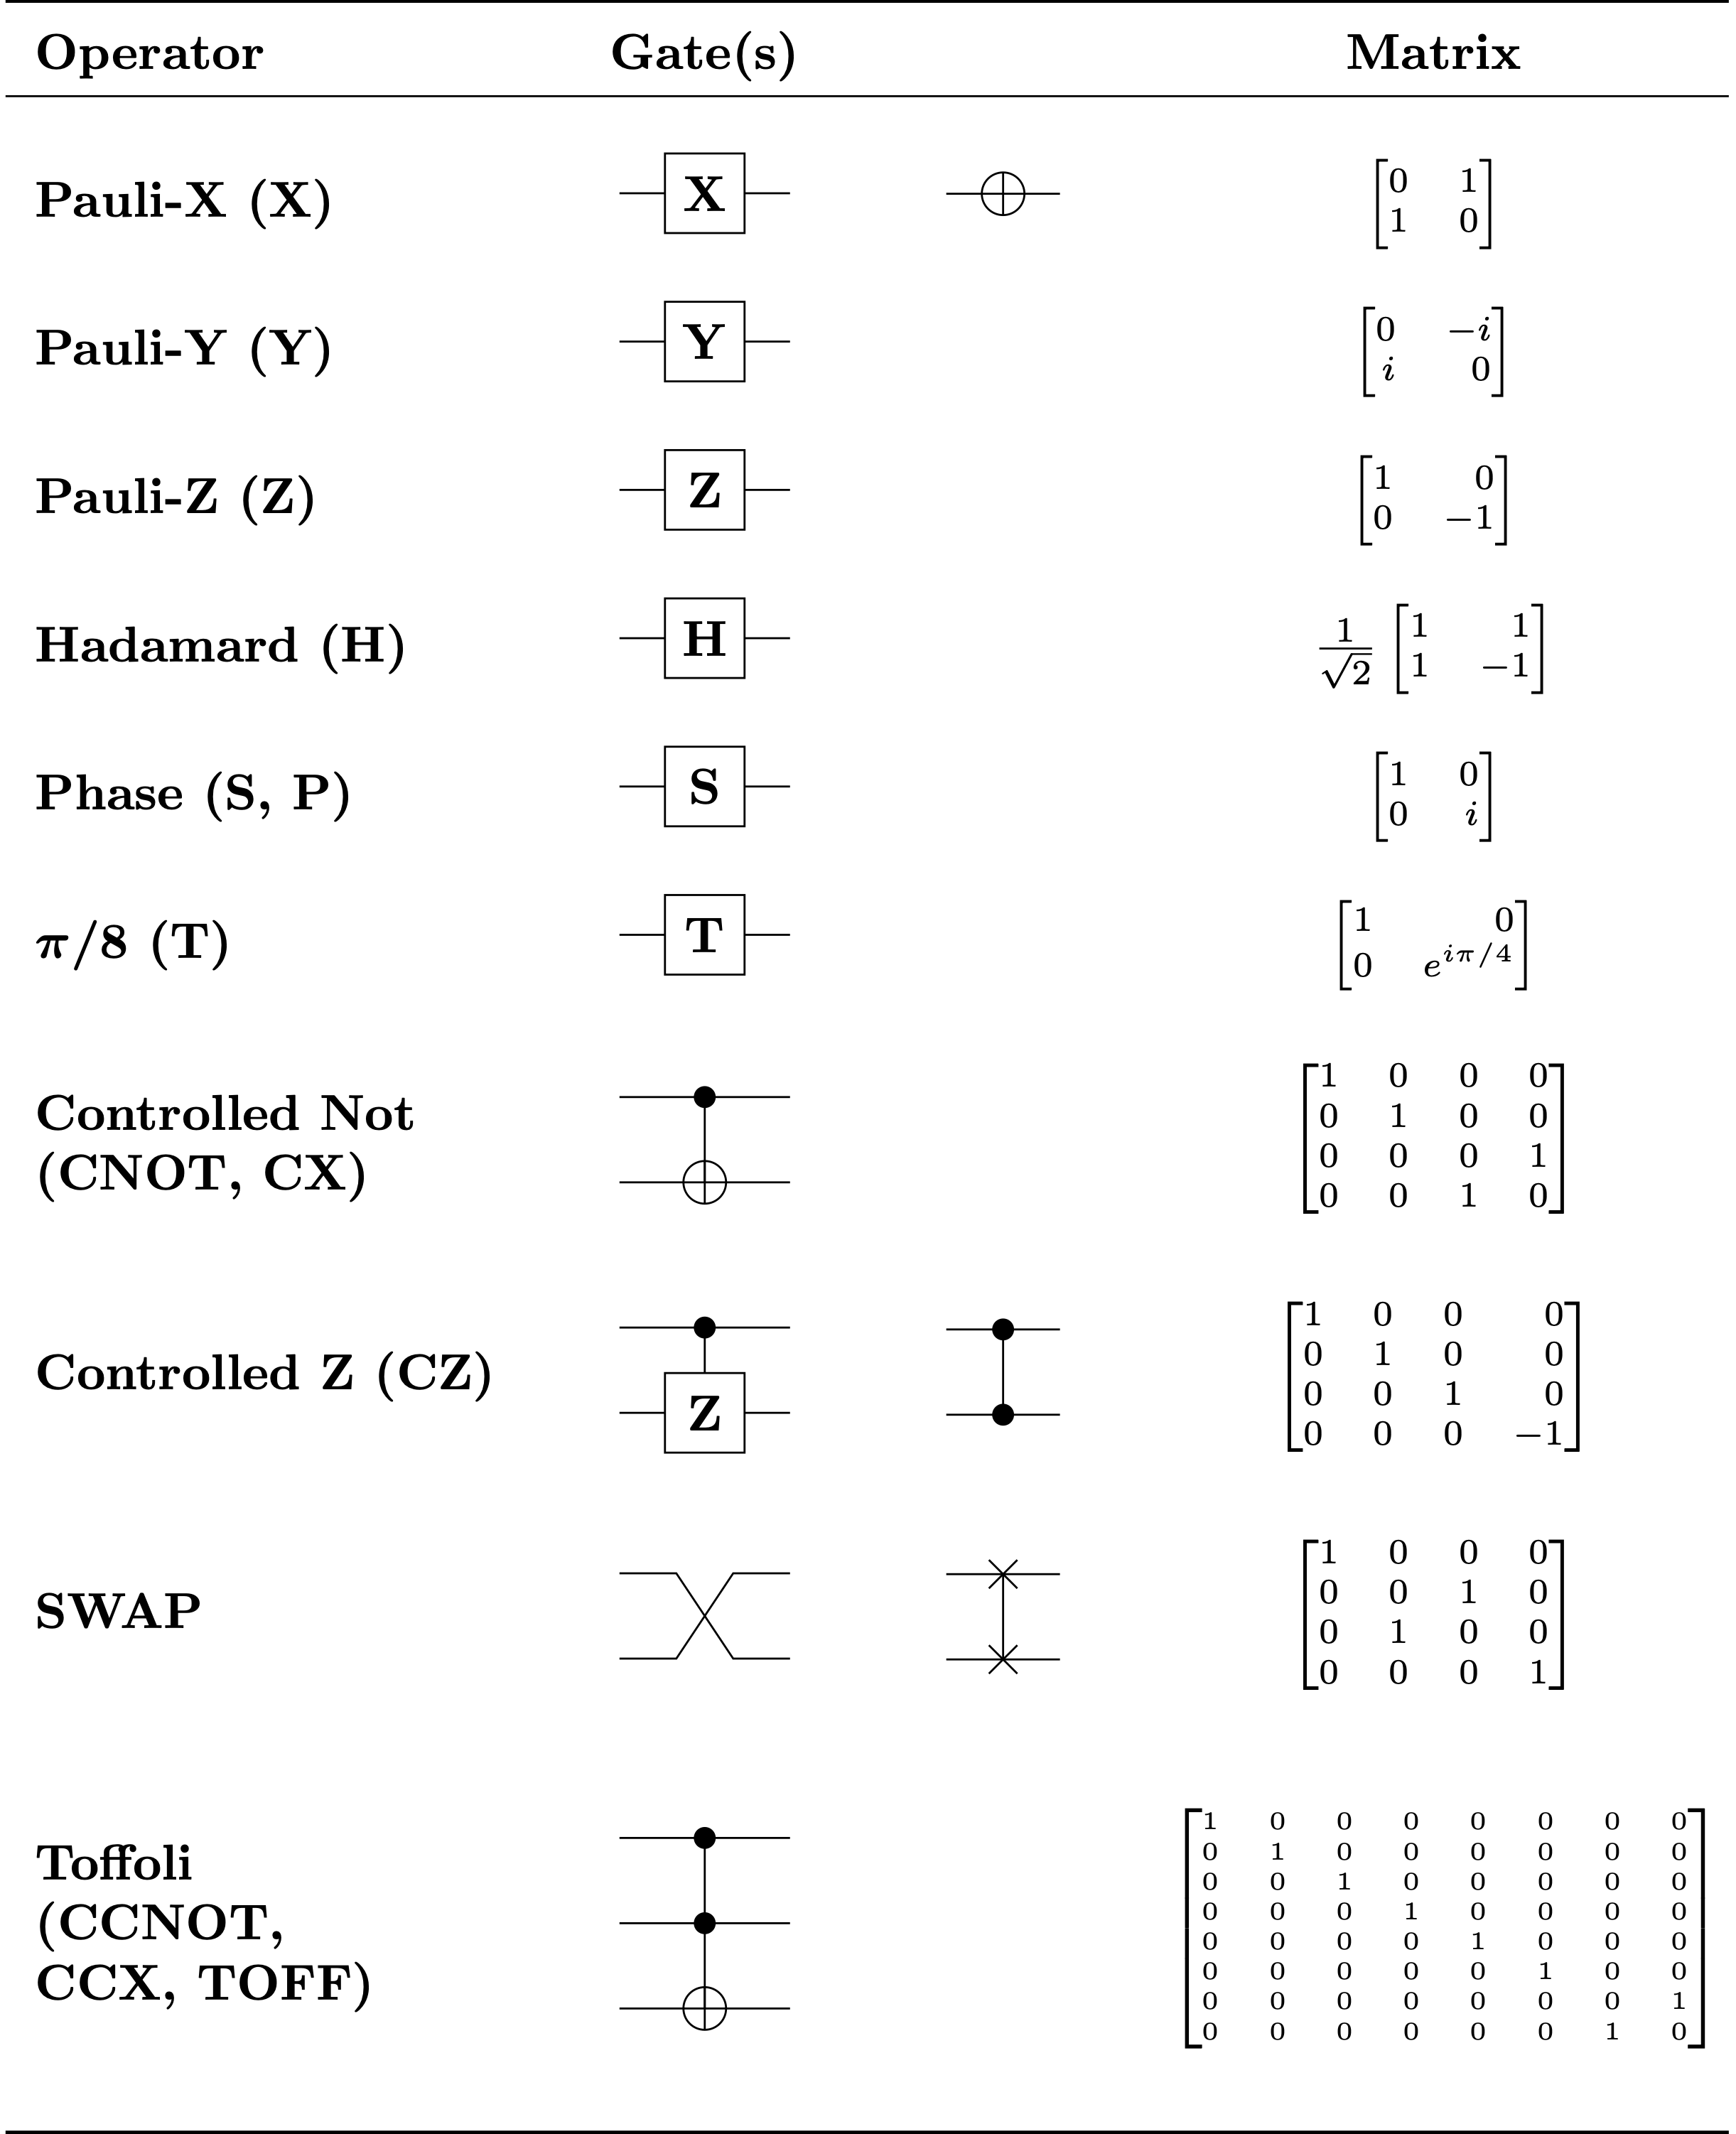
\includegraphics[width = \textwidth]{Images/Quantum_Logic_Gates.png} 
    \caption{Nejpoužívanější kvantové brány. Převzato z \cite{gatesIMG}.
    \todo{TABULKU PŘEDĚLAT, POUŽÍT SMALLMATRIX}}
    \label{fig:gates}
\end{figure}

%\subsection{No-clonning theorem}
%\section{Kvantový paralelismus}
%\todo{\textit{- vyvrátit popular misconception - kvanotvé počítače počítají paralelně všechny možnosti \\
%-mohou pracovat se superponovanými stavy, k nim ale nemáme přístup \\
%-nakonec musíme stejně provést projekční měření a systém nám zkolabuje \\
%-výhodu oproti klasickým získáme tak, že se systémem chytře pracujeme a získáme část skryté informace o superpozici \\
%-popsat Deutsche....možná?
%}}

\section{Kvantové obvody}
Soustava kvantových bran aplikovaná na qubity tvoří \textit{kvantový obvod}. Operace kvantového obvodu je unitární, obvody tedy zachovávají normalizaci stavu a jsou reverzibilní. To plyne z faktu, že kvantové obvody jsou pouze sérií kvantových bran, které jsou unitární, aplikovaných na set qubitů. Z tohoto faktu také vyplývá možnost vyjádřit kvantový obvod unitární maticí rozměru odpovídajícímu počtu qubitů. 


%Jak již bylo naznačeno, k provádění složitějších operací na qubitech složením více kvantových bran slouží \textit{kvantové obvody}. \mk{Ja bych to ppsal z opačného konce, tedy že soustava kvantových bran tvoří obvod.} Na rozdíl od klasických logických obvodů jsou kvantové obvody lineární v tom smyslu, že nepovolují žádné smyčky.\mk{To už také není úplně pravda, jsou tu triky za použití tzv. mid-circuit measurement.} Jejich dalšími důležitými vlastnostmi jsou reverzibilita a unitarita, které plynou z faktu, že kvantové obvody jsou pouze sérií unitárních kvantových bran aplikovaných na set qubitů. Z tohoto faktu také plyne možnost vyjádřit kvantový obvod unitární maticí.

Kvantový obvod se sestává z několika částí. Na vstupu obvodu se nachází \textit{kvantový registr}, soubor qubitů na kterých obvod operuje. Poté je zde samotné tělo obvodu které obsahuje jednotlivé kvantové brány. Obvod obsahuje také \textit{klasický registr}, který slouží pro odečítání hodnot z měření. 

Obvody zakreslujeme pomocí intuitivních diagramů, viz např. Obr. \ref{fig:bell_states}, či Obr. \ref{fig:2qubit_gates_example}. Obvody čteme zleva a jednotlivé horizontální čáry reprezentují qubity. Do obvodu také zakreslujeme měření, a to pomocí následujícího symbolu.
\begin{figure}[H] 
    \centering
    \begin{quantikz}
     & \meter{} & 
    \end{quantikz}
\end{figure}

Důležitými charakteristikami obvodu jsou jeho \textit{hloubka} a \textit{šířka}. Šířka obvodu je počet qubitů na který obvod působí a je dána počtem horizontálních linek v diagramu. Za předpokladu, že kvantový počítač umožňuje aplikovat brány na různé qubity paralelně, představuje hloubka nejdelší možnou cestu obvodem (nejdelší z pohledu počtu bran). Alternativně lze hloubku zavést jako minimální počet časových kroků potřebných k realizaci obvodu, pokud aplikace jedné brány trvá jeden časový krok. Tato definice připouští i možnost, kdy nelze některé brány aplikovat na různé qbity paralelně.

Obvod na Obr. \ref{fig:QCdepth} má hloubku rovnou $5$. Zároveň tento obvod představuje tzv. \textit{parametrizovaný obvod}, který umožňuje interakci s kvantovým počítačem nastavováním parametru $\theta$ v parametrizované bráně $R_z (\theta)$. Parametrizované obvody jsou základním prvkem variačních kvantových algoritmů, kterými se tato práce zabývá.

\begin{figure}[H]
    \centering            
    \begin{quantikz}
            &\gate{H} & \ctrl{1} & & \ctrl{1} & \gate{H} & \\ 
            && \targ{} & \gate{ R_z (\theta) } & \targ{} &&
    \end{quantikz}
    \caption{Příklad kvantového obvodu implementujícího operaci e$^{i\tfrac{\theta}{2} \hat X \otimes \hat Z}$ s hloubkou $5$. }
    \label{fig:QCdepth}
\end{figure}


%\mk{Když takto pěkně popisuje obvody, tak napište i co znamená šířka a hloubka kvantového obvodu.}


%\mk{u obrazku doporucuji vzdy nastavit [htb] za {figure}}

%\subsection{Parametrizované obvody}

\section{Měření na kvantovém počítači} \label{sec:measurement}
%\todo{V závislosti na definici pojmu informace lze stav qubitu interpretovat i tak, že jeho pomocí lze kódovat nekonečně množství informace. To však nelze z qubitu žádným způsobem extrahovat, jelikož měřením lze získat pouze některý ze stavů výpočetní báze. Měřením systém navíc zkolabuje do naměřeného stavu.}


Měření na kvantovém počítači je vždy ve vztahu k nějaké bázi. Nazýváme ji pak \textit{měřící bazí}. Na kvantových počítačích je většinou pro měření užívána standardní báze. Měření qubitu ve standardní bázi matematicky odpovídá aplikaci projekčních operátorů:
\begin{equation}
    \hat{P}_0 = \p{0}, \quad \hat{P}_1 = \p{1}.
\end{equation}
Tyto operace nejsou unitární, nelze je tak interpretovat jako kvantovou bránu. Po měření stav qubitů zkolabuje do naměřeného stavu. 

Stav qubitů, který obvod připravuje lze přibližně zrekonstruovat pomocí opakovaného měření. Kvůli kolapsu stavu po měření musí být však před každým opakování qubity v obvodu připraveny do měřeného stavu znovu. Tímto opakovaným měřením je vygenerována distribuce naměřených výsledků. Příklad obvodu a získané distribuce měřením stavu jím připraveným lze nalézt na Obr. \ref{fig:measurement_example}. Normalizací této distribuce  jsou získány přibližné pravděpodobnosti naměření jednotlivých prvků měřící báze báze. Z nich pak lze odmocněním získat amplitudy náležící jednotlivým stavům měřící báze. Jednotlivým dílčím projekčním měřením bývají nazávány \textit{výstřely} (z angl. shots). Získání pravděpodobnostní distribuce a odhadu stavu opakovanými výstřely bývá často nazýváno pouze \textit{měření}. Čím více výstřelů je provedeno, tím přesnější měření je.


\begin{figure}[H]
\begin{subfigure}{0.4\textwidth}
        \centering
        $\ket{\psi} = \tfrac{1}{\sqrt{2}} (\ket{00} + \ket{11}) \quad \quad$ \\
        \vspace{.5cm}
        \begin{quantikz}
  \lstick{\ket{0}} & \gate{H} & \ctrl{1} &\meter{} & \rstick[2]{\ket{\psi}} \\
  \lstick{\ket{0}} & & \targ{} & \meter{} &  
\end{quantikz}
\vspace{1cm}
    \caption{Obvod připravující měřený stav.}
    \label{fig:measurement_example_circ}
\end{subfigure}
\begin{subfigure}{0.5\textwidth}
    \centering
    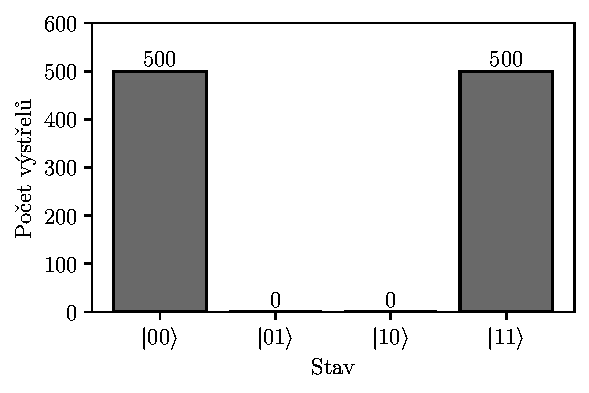
\includegraphics[width=\textwidth]{Images/measurement_plot.pdf}
    \caption{Distribuce výstřelů.}
    \label{fig:measurement_dist}
\end{subfigure}
\caption{Ukázka měření stavu připraveného obvodem \ref{fig:measurement_example_circ}. Obvod stav $\ket{00}$ transformuje do stavu $\ket{\psi}$. V ideálním případě odpovídá distribuce výsledků $1000$ výstřelů grafu \ref{fig:measurement_dist}.}
\label{fig:measurement_example}
\end{figure}

%\todo{Ilustrační příklad toho, že projekci do jiné báze z měření ve standardní bázi prostě nedostanem:}

Měřením v jedné bázi nelze získat podobu tohoto stavu v jiné bázi. To lze snadno ilustrovat na následujícím příkladu. U tomto příkladu je měření provedeno ve standardní bázi, avšak cílem je získat stav v Hadamardově bázi.

Na kvantovém počítači tvořeném jedním qubitem, který nám připravuje systém do neznámého stavu $\ket{\psi}$ bylo provedeno $100000$ měření s následujícími výsledky:
\begin{equation*}
    \ket{0}: 36000 \quad \ket{1}: 64000.
\end{equation*}
Tedy stav $\ket{0}$ s pravděpodobností přibližně $\tfrac{9}{25}$ a $\ket{1}$ s pravděpodobností $\tfrac{16}{25}$. Nyní bychom rádi učinili odhad velikosti projekce $\braket{+}{\psi}$ s využitím tohoto měření. Stav $\ket{\psi}$ můžeme aproximovat jako:
\begin{equation}
    \ket{\psi} \approx \tfrac{3}{5} \ket{0} + e^{i\theta} \tfrac{4}{5} \ket{1}
\end{equation}
Fáze $e^{i\theta}$ nijak neovlivní pravděpodobnosti naměření $\ket{0}$ či $\ket{1}$, její norma je totiž rovna $1$. Nyní použijeme transformační vztahy mezi standardní a Hadamardovou bazí:
\begin{equation}
    \ket{0} = \frac{\ket{+} + \ket{-}}{\sqrt{2}}, \quad
    \ket{1} = \frac{\ket{+} - \ket{-}}{\sqrt{2}}
\end{equation}
Získáme tak stav $\ket{\psi}$ ve tvaru:
\begin{equation}
    \ket{\psi} = \frac{3+4e^{i\theta}}{5\sqrt{2}} \ket{+} + \frac{3-4e^{i\theta}}{5\sqrt{2}} \ket{-}
\end{equation}
Zde ale již Fourierovy koeficienty závisí na fázi $e^{i\theta}$. Pravděpodobnost naměření stavu $\ket{+}$ se tak v závislosti na parametru $\theta$ může pohybovat mezi $\tfrac{2}{100}$ pro $\theta = \pi$ a $\tfrac{98}{100}$ pro $\theta = 0$. Tímto měřením jsme tedy nezískali žádnou informaci o zastoupení $\ket{+}$ a $\ket{-}$ ve stavu $\psi$.

Tento postup je tedy pro měření v jiné než standardní bázi nevhodný. Pro měření v jiné bázi musíme provést dodatečné operace. 

\subsection{Měření v Bázi}
%\todo{-Poro měření v bázi musíme výsledný stav obvodu zrotovat tak, aby báze ve které chceme měřit odpovídala standardní. \\
%-Lze využít invertibility obvodu a přilepit inverzi obvodu pro vytvoření báze ve které chceme měřit}
Kvantový počítač obvykle provádí měření ve standardní bázi. Pro měření stavu připraveného nějakým obvodem v jiné bázi je třeba tento obvod modifikovat přidáním bran, které zajistí rotaci do této jiné báze. Tato dodatečná transformace zobrazuje vektory zvolené měřící báze na vektory standardní měřící báze, které je možné na kvantovém počítači měřit postupem popsaným v předchozí sekci. V konečném efektu, po této transformaci, tak naměření jednotlivých stavů standardní báze odpovídá naměření vektorů zvolené měřící báze. 

K nalezení potřebné transformace lze využít invertibility kvantových obvodů. Obvod pro rotaci do měřící báze totiž odpovídá inverzi obvodu, který zvolenou měřící bázi vytváří ze standardní báze. Příklady měření v Hadamardově a v Bellově bázi lze nalézt na Obr. \ref{fig:hadamard_measurement}, resp. Obr. \ref{fig:bell_measurement}.

\begin{figure}[h]
    \centering
    \begin{quantikz}
   \gate[2]{Q.C.} & \slice[style = black]{} && \gate{H} \gategroup[1, steps = 1, style={dashed}]{\scriptsize Rotace do měřící báze} & \rstick[2]{$\psi^\prime$}
    \end{quantikz}
    \caption{Obvod pro měření stavu připraveného obvodem O.C. v Hadamardově bázi. Po aplikaci dodatečného H odpovídá měření $\ket{0}$ projekci původního stavu připraveného Q.C. do stavu $\ket{+}$, obdobně měření $\ket{1}$ odpovídá projekci do $\ket{-}$.}
    \label{fig:hadamard_measurement}
\end{figure}

%Často také říkáme, že pro měření provedeme rotaci do Z báze. Z báze představuje standartní bázi (vl. vektory $\sigma_z$).

\begin{figure}[h]
    \centering
    \begin{quantikz}
   \gate[2]{Q.C.} & \slice[style = black]{} && \ctrl{1} \gategroup[2, steps = 2, style={dashed}]{\scriptsize Rotace do měřící báze} & \gate{H} & \rstick[2]{$\psi^\prime$} \\
                  &&& \targ{}  &          &  
    \end{quantikz}
    \caption{Obvod pro měření stavu připraveného obvodem O.C. v Bellově bázi. Obvod pro rotaci do měřící báze odpovídá inverzi obvodu pro vytvoření Bellovy báze ze standardní báze (Obr. \ref{fig:bell_states}).}
    \label{fig:bell_measurement}
\end{figure}


%\todo{-Možnost extrahovat informace ze superpozice \\
%-Příklad s fází \\
%-Vysvětlení pomocí diagonalizace \\
%-Vysvětlení pomocí transformace stavů (inverzní obvod k tomu co vytvoří vlastní stavy) \\}

\subsection{Měření operátorů}
\label{sec:mereni_operatoru}
Měřením operátoru rozumíme získání jeho střední (očekávané) hodnoty. Střední hodnota nás zajímá vždy v nějakém stavu. Jelikož se jedná o veličinu statistického charakteru, probíhá měření iterativně. Na kvantovém počítači připravíme stav, ve kterém nás zajímá střední hodnota operátoru a opakovaně tento stav měříme. Pomocí výsledků těchto měření jsme schopni aproximovat očekávanou hodnotu pozorovatelné.

Poznatky této části jsou pouhou aplikací teorie diagonalizace a spektrálního rozvoje. Důkazy k tvrzením lze nalézt ve většině literatury zabývající se lineární algebrou, například \cite{modra_smrt}.

Pozorovatelné odpovídají Hermitovským operátorům. Jsou tedy diagonalizovatelné a jejich vlastní vektory tvoří kompletní ortogonální bázi. Měření v bázi, ve které je hermitovský operátor (pozorovatelná) diagonální (vlastní/přirozená báze) odpovídá měření ve standardní bázi. Abychom tedy mohli provádět měření (ve std. bázi) musíme pozorovatelné diagonalizovat. To lze provést transformací stavu před měřením. Ilustrujme měření pozorovatelné na kvantovém počítači na následujícím příkladu měření $\hat{\sigma}_x$. 

Pauliho brána $X$ je jak unitární, tak hermitovská. Představuje tedy také pozorovatelnou, například v nerelativistické kvantové mechanice ve spinorové reprezentaci pro spin $\sfrac{1}{2}$ projekci spinu do osy $x$. Tuto pozorovatelnou označujeme $\hat{\sigma}_x$. 

Mějme stav $\psi$, který jsme schopni realizovat na kvantovém počítači. Chceme změřit střední hodnotu $\hat{\sigma}_x$ v tomto stavu. Střední hodnotu pozorovatelné lze matematicky vyjádřit pomocí "diracova sandwiche":  %(\todo{možná diracův toast?})

\begin{multline}
    \swich{\psi}{\hat \sigma_x}{\psi} = \bra{\psi} \Bigl( \lambda_+ \p{+}\, + \, \lambda_- \p{-} \Bigr) \ket{\psi} = \bra{\psi} \Bigl( \p{+} \, - \, \p{-} \Bigr) \ket{\psi} = \\ = \braket{+}{\psi}^2 - \braket{-}{\psi}^2.
\end{multline}

Zde v první rovnosti provedeme spektrální rozvoj $\sigma_x$. V poslední rovnosti užijeme hermitovskosti skalárního součinu nad $\mathbb{C}$.

Problém určení střední hodnoty pozorovatelné jsme tedy převedli na určení velikostí projekcí stavu $\psi$ do stavů $\ket{+}$ a $\ket{-}$. Tento problém však byl vyřešen v předchozí podkapitole. Stačí stav $\psi$ zrotovat do správné báze aplikací dodatečné Hadamardovy brány.

\begin{equation}
    \braket{+}{\psi}^2 - \braket{-}{\psi}^2 = \swich{0}{H^\dag}{\psi}^2 - \swich{1}{H^\dag}{\psi}^2 = \braket{1}{\psi^\prime}^2 - \braket{0}{\psi^\prime}^2
\end{equation} 

V tomto případě lze transformaci i vykoukat ze znalosti matice přechodu mezi bazí $\ket{0}$,$\ \ket{1}$ a $\ket{+}$,$\ \ket{-}$. 

Pro obecný operátor $\hat A$ lze tento problém, jak již bylo naznačeno, vyřešit diagonalizací. Pozorovatelné jsou Hermitovské, a tedy vždy diagonalizovatelné. Operátory je možné diagonalizovat přechodem do vlastní báze (tj. báze tvořené vlastními vektory):

\begin{align}
    \swich{\psi}{\hat A}{\psi} &= \swich{\psi}{\hat R ^\dag \hat D \hat R}{\psi} \\
    &= \bra{\psi} \hat{R}^\dag \biggl( \sum_{j=0}^{n-1}  \swich{j}{\hat{D}}{j} \p{j} \biggr) \hat{R} \ket{\psi} \\
    &= \sum_{j=0}^{n-1} D_{jj} \swich{j}{\hat{R}}{\psi}^2 = \sum_{j=0}^{n-1} D_{jj} \braket{j}{\psi^\prime}^2.
\end{align}

V takovém případě je diagonální matice $\hat D$ tvořena vlastními čísly a sloupce $\hat R^\dag$ odpovídají normalizovaným vlastním vektorům. To při znalosti vlastních hodnot operátoru značně ulehčí výpočet jeho střední hodnoty.

Měření střední hodnoty operátoru $\hat{A}$ ve stavu $\psi$ na kvantovém počítači tedy probíhá následujícím způsobem. K obvodu, který připravuje stav $\psi$ přidáme brány odpovídající $\hat{R}$. Počítač tak bude připravovat stav $\ket{\psi^\prime} = \hat{R} \ket{\psi}$. Opakovaným měřením získáme distribuci pravděpodobností naměření jednotlivých vektorů standardní měřící báze $p_i = \braket{i}{\psi^\prime}^2$. Jelikož jsme pomocí rotace $\hat{R}$ přešli do vlastní báze $\hat{A}$, ve které je diagonální, odpovídají vektory standardní měřící báze vlastním hodnotám $\hat{A}$. Střední hodnotu $\hat{A}$ pak spočítáme jako:

\begin{equation}
    \swich{\psi}{\hat{A}}{\psi} = \sum_{i=1}^n a_i p_i,
\end{equation}
kde $a_i$ je vlastní hodnota operátoru $\hat A$ příslušící vlastnímu vektoru $\ket{i}$.

Například tedy výše řešená střední hodnota pozorovatelné $\hat \sigma_x$ ve stavu $\ket{\psi}$ odpovídá měření pozorovatelné $\hat \sigma_z$ ve stavu $\hat{H}\ket{\psi}$ ve standardní bázi, tj užití operátorů $\hat P_0 = \ket{0}\bra{0}$ a $\hat P_1 = \ket{1}\bra{1}$.

Tento postup předpokládá znalost vlastních čísel a vektorů operátoru. Tomu se lze vyhnout rozkladem operátoru na součet Pauliho operátorů. Jejich spektrální rozklady, a tedy i matice $\hat R$ a $\hat D$ jsou známy (Tab. \ref{table:pauli_diagonal}). Pak lze využít linearity střední hodnoty a určit střední hodnotu operátoru jako součet středních hodnot Pauliho operátorů, na jejichž součet je tento operátor rozložen. 

\begin{table}[H]
\centering
\begin{tabular}{c|c|c|c} 
 Operátor & $\hat \sigma$ & $\hat R$ & $\hat D$ \\
 \hline
  & & & \\
 I & $\hat \sigma_x = \begin{pmatrix*}[r] 0 & 1 \\ 1 & 0 \end{pmatrix*}$ & I & I \\
 & & & \\
 X & $\hat \sigma_x = \begin{pmatrix*}[r] 0 & 1 \\ 1 & 0 \end{pmatrix*}$ & H & Z \\
  & & & \\
 Y & $\hat \sigma_x = \begin{pmatrix*}[r] 0 & 1 \\ 1 & 0 \end{pmatrix*}$ & HS$^\dag$ & Z \\
  & & & \\
 Z & $\hat \sigma_x = \begin{pmatrix*}[r] 0 & 1 \\ 1 & 0 \end{pmatrix*}$ & I & Z
\end{tabular}
\caption{Tabulka popisující diagonalizaci Pauliho operátorů.}
\label{table:pauli_diagonal}
\end{table}


%\section{Fyzické kvantové počítače}
%\subsection{Implementace}
%\subsection{Šum}

\chapter{Variační kvantové algoritmy}
\todo{Zmínit, proč výhodné...využijeme kvantový počítač k tomu, co klasicky moc neumíme a pak klasická optimalizace - tu umíme dobře (viz dnešní neuronové sítě a AI)}

\todo{Aplikace čerpat převážně z \cite{cerezo_variational_2021} a z článků tam referencovaných.}
\section{QAOA}
\todo{Stručně popsat algoritmus. Moc nezabíhat do detailů. Zmínit, že je vhodné nejprve přečíst podrobný popis VQE a pak se vrátit k QAOA - lepší kontext a pochopení algoritmu.}
\section{VQLS}
\section{VQE}

Mnoho, nejen fyzikálních problémů, lze převést na hledání vlastních čísel a vektorů nějakého operátoru. Tento typ problémů je řešitelný pomocí algoritmu nazývaného \textit{Quantum Phase Estimation} \textit{(QPE)}. Tento algoritmus umožňuje získat odhad vlastích hodnot unitárních operátorů (respektive jejich fázi na komplexní jednotkové kružnici). Je založen na QFT (\textit{Quantum Fourrier transform}), a tak přináší až exponenciální zrychlení ve srovnání s klasickými algoritmy. QPE je teoreticky dobře popsaný \cite{kitaev_quantum_1995} \cite{nielsen_quantum_2010}, avšak k praktické implementaci vyžaduje kvantové počítače s nízkou chybovostí, které nejsme schopni nyní dosáhnout \cite{mohammadbagherpoor_improved_2019}. Vyvstává tak otázka, zda lze k řešení problému vlastních čísel nějakým způsobem využít dnešních kvantových počítačů, a případně i dosáhnout nějakých výhod vůči klasickým výpočetním metodám. 

Možné řešení této otázky poskytuje algoritmus nazývaný \textit{Variational quantum eigensolver}, zkráceně \textit{VQE}. Jedná se o tzv. hybridní algoritmus, tedy algoritmus kombinující užití klasických a kvantových počítačů. Je realizovatelný i na NISQ počítačích a předpokládá se, že by v blízké době mohl dosáhnout kvantové výhody. VQE patří k relativně mladým algoritmům, první popis byl navržen v roce 2014 \cite{peruzzo_variational_2014}, jeho rozšíření a hlubší teoretický popis pak v roce 2016 \cite{mcclean_theory_2016}. Je tak momentálně aktivně diskutovaným tématem s množstvím publikací (viz např. reference v článku \cite{tilly_variational_2022}, či \cite{tazi_folded_2024}). Existuje mnoho modifikací a rozšíření VQE, které se mohou od zde popisovaného algoritmu více či méně lišit. Základ, který je založen na tzv.\textit{variačním principu} kvantové mechaniky však zůstává pro všechny varianty velmi podobný.
%\mk{Jen dodat větičku, že dnes existuje mnoho  různých variant.}

%\todo{Úvodni kecy, na kvantovém počítači simulujeme stav systému...kvan. počítač roste lineárně s počtem částic. Jsme ale v NISQ éře, tak využijeme k simulaci stavu a poté utečeme do klasicého počítače.}

%\todo{Variational Quantum Eigensolver (VQE) [1] is a quantum algorithm that is a leading contender, if not the top contender, for demonstrating a practical quantum advantage on near-term machines. Unlike traditional quantum algorithms, which have extremely high quantum requirements in terms of gate counts and qubit lifetimes, VQE is feasible with modest quantum resources that are already available on current quantum computers. It attains a lower quantum resource cost in part by structuring computation over a large number of subproblems, each of which can be performed on a quantum computer with modest capabilities. While the low quantum }


\subsection{Variační princip}
Variační princip kvantové mechaniky říká, že střední hodnota pozorovatelné je vždy větší nebo rovna nejmenší vlastní hodnotě této pozorovatelné. Toto tvrzení lze využít k navržení iterativního algoritmu pro získání přibližné hodnoty této nejnižší vlastní hodnoty. To lze speciálně aplikovat na případ energie systému \cite{shankar_principles_1994}. 

Mějme Hamiltonián $\hat{H}$ (či nějakou jinou pozorovatelnou). Důležitým předpokladem je diagonalizovatelnost tohoto operátoru, jeho spektrální rozvoj má pak následující tvar:

\begin{equation}
\hat{H} = \sum_{i=0}^{N-1} E_i \p{i},
\end{equation}

kde $N$ odpovídá dimenzi stavového prostoru systému a $E_i$ je vlastní hodnota příslušná vlastnímu stavu $\ket{i}$. Střední hodnotu Hamiltoniánu v obecném (normalizovaném) stavu $\ket{\psi}$ pak můžeme vyjádřit jako:

\begin{align}
\swch{\psi}{\hat{H}}{\psi}
& = \bra{\psi} \bigg( \sum_{i=0}^{N-1} E_i \p{i} \bigg) \ket{\psi} \\
& = \sum_{i=0}^{N-1} E_i \braket{\psi}{i} \braket{i}{\psi} \\
& = \sum_{i=0}^{N-1} E_i |\braket{i}{\psi}|^2
\end{align}

Položíme-li BÚNO $ E_0 \leq E_i, \ \forall i \in \mathbb{N} $, dostáváme následující odhad:

\begin{align}
\swch{\psi}{\hat{H}}{\psi}
& = \sum_{i=0}^{N-1} E_i |\braket{i}{\psi}|^2 \\
& \geq  \sum_{i=0}^{N-1} E_0 |\braket{i}{\psi}|^2 \\
& = E_0 \sum_{i=0}^{N-1} |\braket{i}{\psi}|^2 \\
& = E_0
\end{align}

Tudíž pro libovolný stav $\ket{\psi}$ platí:
\begin{equation}
\swch{\psi}{\hat{H}}{\psi} \geq E_0.
\end{equation}

Stav $\psi$ lze parametrizovat jako $\psi(\vec\theta)$. Poté můžeme iterativně měřit střední hodnotu operátoru pro různé parametry $\vec{\theta}$ a vždy, když nalezneme novou nejnižší střední hodnotu, získáme přesnější svrchní odhad nejnižší vlastní hodnoty $E_0$.

Hledání základního stavu operátoru $\hat{H}$ s nejmenším vlastním číslem $E_0$ můžeme tedy převést na optimalizační úlohu:
\begin{equation}
\min_{\vec\theta} C(\vec\theta) = 
\min_{\vec\theta} \langle \psi(\vec\theta)|\hat{H}|\psi(\vec\theta)\rangle \geq E_0.
\end{equation}

VQE také řeší toto optimalizační schéma. Simulace stavu $\psi(\vec\theta)$ a změření $\hat{\mathcal{H}}$ v tomto stavu probíhá na kvantovém počítači. Následná optimalizace, tj. výpočet nové sady parametrů $\vec \theta$ je pak provedena na počítači klasickém.  



%\subsection{Quantum phase estimation}
%Popsat stručně algoritmus, proč v blízké době asi nebude (jsme pořád v NISQ éře :-( ) -> motivace pro VQE. 
%Nastínit, že ve VQE kvantový počítač pouze pro reprezentaci Hamiltoniánu a jeho měření - jakmile můžeme, tak utečeme ke klasické části algoritmu.
\subsection{Aplikace VQE}
\cite{bhoy_shell-model_2024}, \cite{kiss_quantum_2022}
Fyzikální, Chemické, Matematické, Finance, Doprava - ideálně dohledat články a tady je oreferencovat.

\chapter{VQE}

V této kapitole je důkladně popsán základ algoritmu VQE. Nejprve je diskutován algoritmus jako celek. Následně, v jednotlivých podkapitolách jsou rozebrány důkladně jednotlivé součásti algoritmu. Prezentované členění algoritmu je převzato z \cite{tilly_variational_2022}. Tento přehledný a obsáhlý souhrnný článek je také doporučen čtenáři k dalšímu studiu. Některé alternativy, či rozšíření algoritmu jsou vysvětleny pouze stručně s odkazem na vhodnou literaturu. Popis je zde zformulován pro Hamiltonián, namísto Hamiltoniánu však může být i libovolná jiná pozorovatelná. 

Jak již bylo nastíněno v předchozí kapitole, VQE je hybridní algoritmus, který slouží k nalezení horní závory nejnižší vlastní hodnoty pozorovatelné. Tento odhad je iterativně zlepšován. 

Nechť $\hat{\mathcal{H}}$ je Hamiltonián systému, jehož základní stav je úkolem nalézt. Mějme dále prostor stavů tohoto systému parametrizován pomocí souboru parametrů $\vec \theta$ a odhad základního stavu s parametry $\vec \theta_0$. V jedné iteraci VQE proběhne výpočet střední hodnoty $\hat{\mathcal{H}}$ v stavu s parametry $\vec \theta_0$, následně je použita nějaká klasická optimalizační metoda, která nalezne novou sadu parametrů $\vec \theta_1$, pro níž je střední hodnota $\hat{\mathcal{H}}$ nižší a stav daný těmito parametry tedy lépe aproximuje základní stav. Pro výpočet nových parametrů je třeba určit očekávanou hodnotu $\hat{\mathcal{H}}$ i pro parametry v okolí $\vec \theta_0$, k čemuž je také použit kvantový počítač. Získaná sada parametrů $\vec \theta_1$ je následně užita v další iteraci jako prvotní odhad. VQE je tudíž heuristický algoritmus, není vždy garantováno dosažení globálního minima v prostoru optimalizovaných parametrů a tedy získání správného výsledku.  

Motivaci k užití kvantového počítače pro reprezentaci stavu a měření Hamiltoniánu v tomto stavu lze nahlédnout na jednoduchém příkladu. Mějme soustavu $N$ částic, z nichž každá má $2$ vlastní stavy, například částice se spinem $\sfrac{1}{2}$. Jedna částice je tedy popsána dvoudimenzionálním Hilbertovým prostorem. Soustava $N$ částic bude pak popsána tenzorovým součinem těchto $2$D prostorů. Jednu částici v tomto případě lze popsat pomocí jednoho qubitu. Pro popis $N$ částic tak bude třeba $N$ qubitů. Avšak Hilbertův prostor popisující soustavu $N$ částic bude $2^N$-dimenzionální. Při popisu na klasickém počítači by tedy bylo třeba pro kompletní popis systému $2^N$ amplitud, tedy se jedná o problém s exponenciální náročností. Jednou s největších výhod VQE tak je škálovatelnost vůči velikosti systému.

VQE však nepřináší exponenciální výhodu. Důvodem je fakt, že Hamiltonián musí být nejprve rozložen na součet tzv. \textit{Pauliho řetězců} jejichž počet je řádu $\mathcal{O}(poly(N))$. Důvod k tomuto rozkladu bude popsán níže. K určení očekávané hodnoty Hamiltoniánu bude tedy s užitím kvantového počítače třeba $\mathcal{O}(poly(N))$ operací, při výpočtu na klasickém počítači by oblo operací třeba $\mathcal{O}(2^N)$. VQE tedy může mít až polynomiální výhodu.

    \begin{figure}[h]
        \centering
        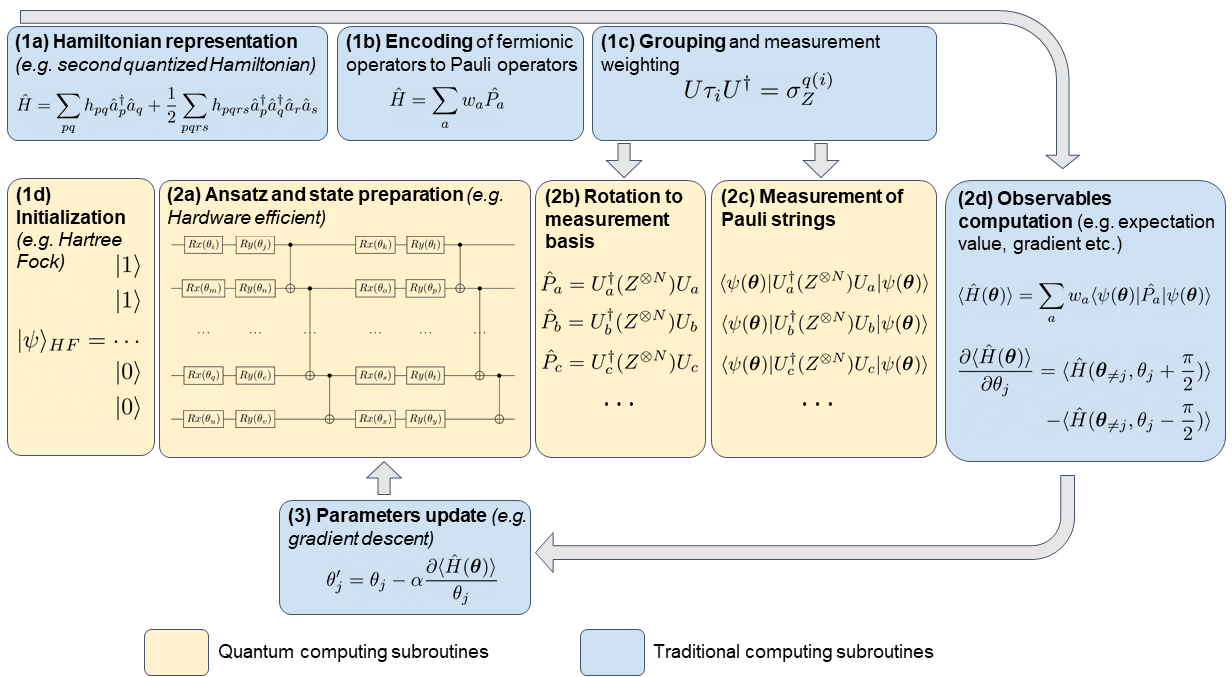
\includegraphics[width=\textwidth]{Images/VQE_pipeline.png}
        \caption{Shrnutí VQE, ukradeno z \cite{tilly_variational_2022}, ideálně PŘEKRESLIT do vektoru a udělat hezčí.}
        \label{fig:VQE_diagram}
    \end{figure}
\section{Popis algoritmu}
V této části bude VQE rozdělen na několik částí, které budou dále důkladně rozebrány. Názorné schéma algoritmu lze nalézt na Obr. \ref{fig:VQE_diagram}. Nejprve je třeba vyjádřit řešený problém pomocí Hamiltoniánu. Ten je pak enkódován pomocí Pauliho operátorů tak, aby mohl být reprezentován na kvantovém počítači. Následně je vytvořen parametrizovaný kvantový obvod, tzv. \textit{ansatz}, který z výchozícho stavu (např. $\ket{0}^{\otimes N}$) vytvoří parametrizovaný stav, který alespoň částečně pokrývá prostor zkoumaného Hamiltoniánu. V tomto parametrizovaném stavu bude probíhat měření Hamitoniánu realizované rotací do báze ve které je Hamiltonián diagonální a opakovaným projekčním měřením. Určená očekávaná hodnota je pak využita k získání nových parametrů ansatzu pomocí klasického \textit{optimizéru}. Následuje stručný popis částí diagramu na Obr. \ref{fig:VQE_diagram}.
\begin{itemize}
    \item \textbf{Reprezentace Hamiltoniánu:} Problém je třeba nejprve formulovat jako úlohu na hledání základního stavu. Dále je třeba zvolit vhodnou bázi, ve které bude vyjádřen Hamiltonián zkoumaného systému. Častou volbou pro sféricky symetrické systémy bývají například bazické funkce tvořené kulovými (někdy nazývané sférické harmonické) funkcemi násobené radiálními funkcemi. Jednočásticové stavy (orbitaly) jsou tedy obvykle známy. Pro více částicové systémy bývá báze často vytvořena z těchto jednočásticových bazických funkcí. Další vlastností, kterou musí reprezentace reflektovat je symetrie, resp. antisymetrie systému vůči výměně částic. Například systém fermionů (elektronový obal atomu, nukleony v jádře atd.) musí být vůči záměně dvou částic antisymetrický. Existují de facto dvě možnosti, jak toho dosáhnout. První z nich je tuto antisymetrii vynutit ve vlnových funkcích, druhou možností je ji realizovat definicí operátorů. Tyto dvě reprezentace se popořadě nazývají první a druhé kvantování, tyto názvy mají historický původ. Pro VQE bývá Hamiltonián obvykle reprezentován pomocí druhého kvantování. Hamiltonián je tak vyjádřen pomocí kreačních operátorů $\hat a^\dag_j$ a anihilačních operátorů $\hat a_j$, jejichž působení odpovídá přidání respektive odebrání částice v $j$-tém stavu (tj. stavu popsaném $j$-tou bazickou funkcí). Antisymetrie je pak vynucena antikomutačními relacemi těchto operátorů. 
    \item \textbf{Enkódování Hamiltoniánu:} Dále je třeba Hamiltonián nějakým způsobem enkódovat tak, aby jej bylo možno měřit na kvantovém počítači. Toho je docíleno vyjádřením Hamiltoniánu pomocí Pauliho řetězců pro $N$ qubitů $\hat{P_i} \in \{ I, X, Y, Z \} ^{\otimes N}$. To je možné mimo jiné proto, že Pauliho operátory spolu s jednotkou tvoří bázi operátorů na daném prostoru. Hamiltonián má tak tedy podobu lineární kombinace $\hat P_i$ Jednotlivé Pauliho řetězce pak lze vyjádřit jako kvantové obvody. V prvním kvantování je mapování provedeno přímou ekvivalencí bazických stavů a výpočetní bazí kvantového počítače. Projekční operátory tak jsou vyjádřeny pomocí Pauliho operátorů. V druhém kvantování jsou kreační a anihilační operátory zobrazeny na kombinace Pauliho operátorů, a to takovým způsobem, aby byla zachována případná antisymetrie fermionických systémů. Příklady dvou takových zobrazení jsou Jordan-Wigner \cite{jordan_uber_1928} a Bravyi-Kitaev \cite{bravyi_fermionic_2002} transformace, které jsou zároveň nejpoužívanějšími.
    \item \textbf{Strategie měření:} Měření operátorů (viz kapitola \ref{sec:mereni_operatoru}) probíhá rotací stavů do báze, ve které je operátor diagonální. Hamiltonián je ve VQE vyjádřen pomocí Pauliho operátorů, pro které jsou diagonalizace známé. Linearita střední hodnoty umožňuje rozdělit měření střední hodnoty Hamiltoniánu na měření středních hodnot Pauliho řetězců z rozkladu v předchozím kroku. Tato rotace do báze je realizována kvantovým obvodem (viz \ref{table:pauli_diagonal}), kterým bude transformován stav ve kterém probíhá měření. Opakovaným projekčním měřením tohoto zrotovaného stavu je získána pravděpodobnostní distribuce, a z ní již lze určit očekávané hodnoty Pauliho řetězců. Měření lze dále zefektivnit, některé řetězce jsou totiž diagonalizovatelné současně a jejich střední hodnotu lze určit pomocí stejné pravděpodobnostní distribuce. Takové řetězce budou vzájemně komutovat, a tak lze využít vlastností Lieovy algebry Pauliho matic k jejich identifikaci. Tato seskupení jsou netriviální a existuje jich mnoho, identifikace optimálního seskupení je předmětem současného výzkumu \cite{gokhale_minimizing_2019}, \cite{huggins_efficient_2021}, \cite{hamamura_efficient_2020}, \cite{gokhale_on3_2019}.
    \item \textbf{Ansatz:} Hlavní podstatou VQE je procházení Hilbertova prostoru Hamiltoniánu pomocí parametrizovaných stavů. Optimalizací parametrů je pak nalezeno (přibližné) minimum střední hodnoty Hamiltoniánu. Toto minimum pak představuje odhad energie základního stavu, jehož odhad je získán dosazením parametrů pro nalezené minimum. Kvantový obvod, který tento stav připravuje je nazýván \textit{ansatz}. Ansatz do velké míry ovlivňuje náročnost a přesnost VQE. Kvalitu ansatzu vyjadřuje to, jak dobře dokáže obsáhnout Hilbertův prostor zkoumaného Hamiltoniánu a to, jak dobře trénovatelný (tj. jak rychle, jak přesně a zda vůbec lze nalézt minimum). Pokrytí stavového prostoru by mělo být dostatečné, aby bylo garantováno, že bude dobrým modelem základního stavu, zároveň však musí být mohutnost ansatzu v souladu s možnostmi současných kvantových počítačů a optimalizačních metod. V praxi může být volba ansatzu motivována buď konkrétním fyzikálním problémem, či hardwarem kvantového počítače. V první možnosti ansatz zaveden v souladu se známými stavy Hamiltoniánu. V druhé možnosti je zase navržen tak, aby jej bylo možné optimálně realizovat na daném kvantovém hardwaru.
    \item \textbf{Optimalizace parametrů:} V závěru jedné iterace je třeba určit parametry ansatzu pro další iteraci.
    Optimalizace parametrů je již čistě klasická část VQE. Výběr optimizéru nicméně značně ovlivňuje přesnost, úspěšnost i náročnost algoritmu. Optimizér udává, kolik měření je nutno v jedné iteraci provést a také, kolik iterací je třeba k dosažení konvergence. Optimizéry bývají často navrženy specificky tak, aby kontrovaly různé optimalizační problémy, například sedla v optimalizační krajině, či velké množství lokálních minim. Optimizérů existuje velké množství \cite{bonet-monroig_performance_2023} a správný výběr je esenciální pro efektivní fungování VQE.
\end{itemize}


\section{Enkódování Hamiltoniánu}
Před řešením problému pomocí VQE je třeba nejprve formulovat Hamiltonián s tímto problémem spojený. Z principu korespondence lze v kvantové mechanice vyjádřit Hamiltonián analogicky s klasickou mechanikou \cite{shankar_principles_1994}. Tedy pro potenciál nezávislý na hybnostech jako součet kinetické energie $\hat T$ a potenciální energie $\hat V$:
\begin{equation}
    \hat H = \hat T + \hat V,
\end{equation}
pro N částic má v souřadnicové reprezentaci operátor kinetické energie tvar:
\begin{equation}
    \hat T = \sum_{i=1}^{N} \frac{\hat p_i^2}{2m_i} = -\sum_{i=1}^{N} \frac{\hbar^2}{2m_i}\nabla^2.
\end{equation}
Pro více částic lze dále Hamiltonián rozepsat jako:
\begin{equation}
    \hat H = \hat T + \hat V + \hat W = \hat T + \sum_i \hat v_i + \frac{1}{2} \sum_{i,j} w_{ij},
    \label{eq:hamiltonian}
\end{equation}
kde je uvažována vzájemná interakce maximálně dvou částic. Člen $\hat V = \textstyle \sum_i \hat v_i$ představuje externí potenciál a je dán součtem operátorů $\hat v_i$ působících pouze na jednu částici. Člen $\hat W = \textstyle \sum_{i,j} w_{i,j}$ je nazýván párový interakční člen a operátory $\hat w_{i,j}$ působí na dvě částice.

Potenciál je specifický pro každý systém a jeho správná volba je základem dobrého popisu. V tomto kroku často dochází k aproximacím, které zjednodušují řešení. Tyto aproximace mohou mít různou podobu. Například rozdělení Hamiltoniánu na součet několika členů, kde je interakce mezi těmito členy zanedbána. Příkladem je například Born-Oppenheimer aproximace pro molekulární Hamiltoniány \cite{born_zur_1927}, ve které je uvažována kinetická energie pouze elektronového obalu a potenciál je rozdělen na coloumbický interakční člen párů elektron-elektron a interakční člen párů elektron-nukleon. Je tak uvažována vždy pouze interakce dvou částic. Dále mohou být zahrnuty také spinové, vibrační či rotační členy.

Další, velmi častou aproximací je nahrazení vzájemné interakce částic globálním potenciálem. Bývá používána například pro jaderné modely nebo dále rozebírané vektorové mezony. Z pohledu jedné částice tak inerakce s ostatními částicemi odpovídá uvěznění v potenciálové jámě. Potenciál bývá často sféricky symetrický a nejjednoduššími volbami jsou sféricky symetrická jáma, pole izotropního harmonického oscilátoru $V \propto r^2$ a analogie Coloumbického potenciálu $V \propto \tfrac{1}{r}$.

\subsection{Částice ve sféricky symetrickém potenciálu}
Sférická symetrie umožňuje značné zjednodušení řešení Schrödingeroy rovnice. Křešení lze postupovat vícero způsoby například čistě matematicky, užitím separace proměnných, nebo více fyzikálně, hledáním vlastních stavů úplné množiny pozorovatelných $\{ \hat L^2,\, \hat L_3,\ \hat H \}$. Hamiltonián je pak součtem radiální a úhlové části, výsledné vlnové funkce jsou zase součinem radiálně závislé a úhlově závislé části. Úhová část opdovídá vlastním stavům $\hat L^2$. Radiální část vlnové funkce je řešením jednodimenzionální schrödingerovy rovnice pro částici v efektivním potenciálu $\hat V_\mathrm{eff} = \hat V + \tfrac{\hbar^2 j(j+1)}{2mr^2}$, kde $\hat V$ je původní potenciál \cite{shankar_principles_1994}.

Problém lze atakovat čistě matematicky pomocí separace proměnných. Alternativně lze postupovat fyzikálně motivovaným přístupem a postupně hledat vlastní čísla a vlastní vektory úplné množiny pozorovatelných ($\hat L_z$, $\hat L^2$, $\hat H$). Ty mají v reprezentaci sférických souřadnic tvar:

\begin{equation}
    \hat{L}_z =-i\hbar\frac{\partial}{\partial\varphi}
\end{equation}

\begin{equation}
    \hat{L}^{2}=-\hat{h}^{2}\left[\frac{1}{\sin^{2}\theta}\frac{\partial^{2}}{\partial\varphi^{2}}+\frac{1}{\sin\theta}\frac{\partial}{\partial\theta}\left(\sin\theta\frac{\partial}{\partial\theta}\right)\right]
\end{equation}

\begin{equation}
    \hat{H}=-\frac{\hbar^{2}}{2M}\left[\left(\frac{\partial^{2}}{\partial r^{2}}+\frac{2}{r}\frac{\partial}{\partial r}\right)-\frac{1}{\hbar^{2}r^{2}}\hat{L}^{2}\right]+\hat{V}(r)
\end{equation}

Vlastní čísla $\mu$ a vlastní funkce $\Psi$ operátoru $\hat L_z$ lze snadno nalézt řešením Schrödingerovy rovnice \cite{shankar_principles_1994}:
\begin{equation}
    -i\hbar\frac{\partial}{\partial\varphi}\Psi(r,\theta,\varphi) = \mu \Psi(r,\theta,\varphi)
\end{equation}
Jsou číslovány tzv. \textit{magnetickým kvantovým číslem} $m$ a mají tvar: 
    \begin{equation} \begin{split}
        \Psi_m(r,\theta,\varphi) &= \chi(r,\theta)e^{i m\varphi},\  m\in\bf{\mathbb{Z}} \\
        \mu_n &= m\hbar.
        \label{eq:Lz_eigen}
    \end{split} \end{equation}

\begin{itemize}
        \item Známe vl. čísla $\hat L_z$: $\mu=m\hbar$ \textrightarrow magnetické kvantové číslo m
        \item Vlastní funkce operátoru $\hat L_z$:
    \end{itemize}
    \begin{equation}
        \Psi(r,\theta,\varphi) = \chi(r,\theta)e^{i m\varphi},\  m\in\bf{\mathbb{Z}},
    \end{equation}

\begin{itemize}
    \item Substitucí do Schrodingerovy rce pro $\hat L^2$ a zavedením proměnné $t = \cos \theta$ dostaneme tzv. Legenderovu dif. rovnici
    \item Řešením Legenderovy polynomy \textrightarrow kulové funkce $Y_{l, m}\left(\theta,\varphi\right)$
    \item Vl. čísla $\hat L^2$ \textrightarrow  vedlejší kvantové číslo $l$
\end{itemize}
    
    \begin{equation}
\lambda=l(l+1)\hbar^{2},\ \ l\in\mathbb{Z}_{+}, \ \ m\in\mathbb{Z},\ \  |m|\leq l.
    \end{equation}

\begin{itemize}
        \item Máme tedy společné vl. vektory:
    \end{itemize}
    \begin{equation}
        \Psi(r,\theta,\varphi)= \tfrac{1}{r} R(r)Y_{l m}(\theta,\varphi)
    \end{equation}

    \begin{itemize}
        \item Zbývá vyřešit závislost na $r$
        \item Záleží na konkrétním potenciálu $V(r)$, substituce $\Psi(r,\theta,\varphi)$ do rce. pro $\hat H$ \textrightarrow rovnice pro částici v efektivním potenciálu $V_{ef}$
    \end{itemize}

    \begin{equation}
        V_{\mathrm{ef}}(r)=V(r)+\frac{\hbar^{2}}{2M}\frac{l(l+1)}{r^{2}}
    \end{equation}

    \begin{equation}
        -\frac{\hbar^{2}}{2M}R^{\prime\prime}(r)+V_{\mathrm{ef}}(r)R(r)=E_n R(r)
    \end{equation}

    \begin{itemize}
        \item Řešením pro konkrétní potenciál - energetické hladiny $E_n$ \textrightarrow hlavní kvantové číslo $n$, svázání E a l,m

    \end{itemize}

Struktura momentu hybnosti tedy plyne čistě ze sférické symetrie systému a nezávisí na potenciálu. Řešení sféricky symetrických úlohy bude tedy mít vždy podobu orbitalů daných kulovými funkcemi v různých energetických hladinách číslovaných pomocí vedlejšího kvantového čísla $l$ a magnetického kvantového čísla $m$. Vlastní stavy energie na druhou stranu závisí na potenciálu, a kvůli odstředivému členu i na velikosti momentu hybnosti.

\todo{Naznačit řešení, odkázat se na \cite{shankar_principles_1994}}
\todo{Napsat výsledky pro Izotropický harmonický oscilátor, vodíkový atom (elektron v columbickém potenciálu), napsat kulové funkce a }
\subsection{Nerozlišitelné částice}
Kvantové částice stejného druhu jsou nerozlišitelné. Každá z nich tedy musí být popsána stejnou sadou vlnových funkcí řešících jednočásticovou Schrödingerovu rovnici. Společný stav systému více nerozlišitelných částic pak bude popsán tenzorovým součinem těchto jednočásticových stavů. Dle tzv. \textit{symetrizačního postulátu} je lze rozdělit do dvou skupin podle chování jejich společné vlnové funkce při záměně dvou částic. Vlnová funkce je symetrická pro \textit{bosony} a antisymetrická pro \textit{fermiony}. Je-li tedy $\ket{\psi}$ množina normalizovaných stavů pro jednu částici, platí pro dvě nerozlišitelné částice následující:
\begin{equation}
    \ket{\psi_1, \psi_2} = \xi \ket{\psi_2, \psi_1}, 
\end{equation}
kde $\xi = 1$ pro bosony a $\xi = -1$ pro fermiony. Společný stav takových dvou částic tedy musí mít tvar:
\begin{equation}
    \ket{\psi_1, \psi_2} = \frac{1}{\sqrt{2}}(\ket{\psi_1}\otimes\ket{\psi_2} + \xi \ket{\psi_2}\otimes\ket{\psi_1}),
\end{equation}
Pro vlnovou funkci v poziční bázi platí:
\begin{equation}
    \psi(x_1,x_2) = \braket{x_1,x_2}{\psi_1, \psi_2} = \frac{1}{\sqrt{2}} (\braket{x_1}{\psi_1}\braket{x_2}{\psi_2} + \xi \braket{x_1}{\psi_2}\braket{x_2}{\psi_1})
\end{equation}
Společný stav pro $N$ nerozlišitelných částic má obecně tvar \cite{zhang_permanent_2022}:

\begin{equation}
\ket{\psi_1,\psi_2,\ldots \psi_N} = \sqrt{\frac{\prod_{i=0}^\infty n_i!}{N!}} \sum_{\mathcal{P}} \xi^{\tfrac{1}{2} \mathrm{sgn} (\mathcal{P})} \ket{\psi_{\mathcal{P}_1}} \otimes \ket{\psi_{\mathcal{P}_2}} \otimes \ldots \otimes \ket{\psi_{\mathcal{P}_N}},
\label{eq:N_particle_state}
\end{equation}
kde $n_i$ představuje počet částic v daném stavu. Pro fermiony tedy $n_i \in \{ 0,\, 1 \}$, sumace probíhá přes všechny možné permutace a $\mathrm{sgn} (\mathcal{P})$ je znaménko dané permutace. V případě fermionů je tento společný stav $N$ částic znám jako tzv. \textit{Slaterův determinant}. Tento způsob vynucení (anti)symetrie definicí vlnové funkce bývá nazývaný \textit{první kvantování}. Alternativní popis, nazývaný \textit{druhé kvantování} (anti)symetrii vynucuje vhodnou definicí operátorů.

\subsection{První kvantování}
V prvním kvantování jsou stavy systému $N$ částic popsány pomocí definice (\eqref{eq:N_particle_state}), která vynucuje (anti)symetrii vůči záměně částic. Hamiltonián (\eqref{eq:hamiltonian}) pak lze rozepsat pomocí projekčních operátorů a maticových elementů:
\begin{equation}
    h_{pq} = \swich{\psi_p}{\hat T + \hat V}{\psi_q},
\end{equation}
\begin{equation}
    h_{pqrs} = \swch{\psi_p \, \psi_q}{\, \hat W \, }{\psi_r \, \psi_s},
\end{equation}
\begin{equation}
    \hat H = \sum_{i=1}^N \sum_{p,q} h_{pq} \pp{\psi^{(i)}_p}{\psi^{(i)}_q} + \frac{1}{2} \sum_{i \neq j}^N \sum_{p,q,r,s} h_{pqrs} \pp{\psi^{(i)}_p \psi^{(j)}_q}{\psi^{(i)}_r \psi^{(j)}_s},
    \label{eq:first_quantized_hamiltonian}
\end{equation}
kde indexy $i$ a $j$ odpovídají jednotlivým částicím a $p,\, q, \, r, \, s$ číslují jednočásticové stavy.

Je-li jednočásticových bazických stavů $n$, lze je přímo ztotožnit se stavy $\log_2(n)$ qubitů. Například $\ket{\psi_1} = \ket{00 \ldots 00}$, $\ket{\psi_2} = \ket{00 \ldots 01}$ a tak dále \cite{abrams_simulation_1997}. Pro $N$ částic je tedy třeba $m = N\log_2(n)$ qubitů. 
Projekční operátory v (\eqref{eq:first_quantized_hamiltonian}) pak budou odpovídat projekčním operátorům na příslušné stavy $m$ qubitů \cite{mcardle_quantum_2020}, \cite{nielsen_quantum_2010}. Tyto projekční operátory lze rozložit na tenzorový součin projekčních operátorů na prostoru jednoho qubitu. Jednoqubitové projekční operátory lze zase vyjádřit následovně pomocí Pauliho operátorů \cite{nielsen_quantum_2010}:
\begin{equation}
    \p{0} = \tfrac{1}{2} (\hat I + \hat Z), \quad \pp{0}{1}= \tfrac{1}{2} (\hat X + i\hat Y), \quad \pp{1}{0}= \tfrac{1}{2} (\hat X - i\hat Y) , \quad \p{1} = \tfrac{1}{2} (\hat I - \hat Z).
\end{equation}
Hamiltonián v prvním kvantování lze tedy enkódovat jako lineární kombinaci tenzorových součinů Pauliho operátorů. Hamiltonián tak lze reprezentovat na kvantovém počítači pomocí Pauliho bran. Toto enkódování bývá často užíváno pro systémy bosonů.

\subsection{Druhé kvantování}
Antisymetrii lze vynutit alternativně definicí operátorů, nikoliv vlnových funkcí. Jsou zavedeny tzv. \textit{kreační} a \textit{anihilační} operátory pomocí nichž jsou následně vyjádřeny libovolné jiné operátory pozorovatelných, tento formalismus má počátky již ve 30tých letech minulého století \cite{jordan_uber_1928}. V druhém kvantování jsou stavy systému reprezentovány pomocí tzv. \textit{obsazovacích čísel}. Formální odvození následujících vztahů lze nalézt ve většině pokročilejších učebnicích kvantové mechaniky, například \cite{shankar_principles_1994}, \cite{altland_condensed_2010}.    

Nechť je $\{ \ket{\psi_1},\, \ket{\psi_2}\ldots \}$ množina jednočásticových stavů. Pro Hilbertův prostor $N$ takových nerozlišitelných částic $\mathcal{F}^N$ lze vygenerovat bázi jako permutace tenzorového součinu $N$ jednočásticových stavů, viz předchozí podkapitola. Alternativní bázi s poněkud menší redundancí lze zkonstruovat reprezentací pomocí \textit{obsazovacích čísel}, kde \textit{obsazovací číslo} $n_i$ odpovídá počtu částic systému v jednočásticovém stavu $\ket{\psi_i}$. Tato báze prostoru $\mathcal{F}^N$ má tvar $\{ \ket{n_1,\, n_2\ldots} | \textstyle \sum n_i = N \}$.  Společný stav $N$ částic (\eqref{eq:N_particle_state}) pak bude mít tvar následující superpozice:
\begin{equation}
    \ket{\psi} = \sum_{\sum n_i = N} c_{n_1, n_2,..}\ket{n_1, n_2,...}.
\end{equation}
Složením $\mathcal{F}^N$ pro všechny možné počty částic $N$ a přidáním \textit{vakuového stavu} $\ket{0}$, který neobsahuje žádné částice (tj. $N = 0$) vzniká \textit{Fockův prostor} $\mathcal{F}$:
\begin{equation}
    \mathcal{F} = \bigoplus_{N=0}^{\infty} \mathcal{F}^N.
\end{equation}

Prostor $\mathcal{F}$ je tedy prostor pro variabilní počet částic. $\{ \ket{n_1, n_2,...} |\, n_i \in \mathbf{N} \}$ je jeho báze. Libovolný stavový vektor lze rozepsat superpozicí:
\begin{equation}
    \ket{\psi} = \sum_{n_1,n_2,..} c_{n_1, n_2,..}\ket{n_1, n_2,...}.
\end{equation}
Operátory $\hat a^\dag_i: \ \mathcal{F} \rightarrow \mathcal{F}$ se nazývají \textit{kreační operátory}. Aplikace $\hat a^\dag_i$ představuje přidání částice do $i$-tého stavu. Tyto operátory jsou definovány následujícím způsobem:
\begin{equation}
    \hat a^\dag_i \ket{n_1,...,n_i,...} = \sqrt{n_i+1} \xi^{s_i} \ket{n_1,...,n_i+1,...},
\end{equation}
kde $\xi = 1$ pro bosony a $\xi = -1$ pro fermiony a $s_i = \textstyle \sum_{K=1}^{i-1}n_k$. V případě fermionů je zvyšování obsazovacího čísla chápat jako modulo $2$, tedy $1+1=0$ a $0+1=1$.

Opakovanou aplikací kreačního operátoru lze vygenerovat celou bázi $\mathcal{F}:$
\begin{equation}
    \ket{n_1,n_2,..} = \prod_i \tfrac{1}{\sqrt{n_i!}} (\hat a^\dag_i)^{n_i} \ket{0}.
\end{equation}
Pro hermitovsky sdružený operátor $\hat a_i$ k $\hat a^\dag_i$ lze odvodit \cite{shankar_principles_1994} následující:
\begin{equation}
    \hat a_i \ket{n_1,...,n_i,...} = \sqrt{n_i} \xi^{s_i} \ket{n_1,...,n_i-1,...},
\end{equation}
nazývá se \textit{anihilační operátor} a jeho akce odpovídá odstranění částice v $i$-tém stavu. Aplikace $\hat a_i$ na $\ket{0}$ stav anihiluje. Tedy:
\begin{equation}
    \hat a_i \ket{0} = 0.
\end{equation}
V systémech fermionů bývají anihilační a kreační operátory souhrnně nazývané fermionické operátory. Pro $\hat a_i$ a $\hat a^\dag_i$ platí následující (anti)komutační relace:
\begin{equation}
    [\hat a^{\ }_i,\hat a^\dag_{j}]_\xi = \delta_{ij},\quad [\hat a_i,\hat a_j]_\xi = 0, \quad [\hat a^\dag_i,\hat a^\dag_j]_\xi = 0,
    \label{eq:relace_kreacni_anihilacni_op}
\end{equation}
kde index $\xi$ značí, že pro fermiony jde o antikomutátor a pro bosony o komutátor. Tyto relace definují algebru, která plně charakterizuje akci těchto operátorů.

Pro vyjádření pozorovatelných v druhém kvantování je nejprve třeba zavést operátor obsazovacího čísla a počtu částic a změnu páze anihilačního a kreačního operátoru. Dále mohou být pro přehlednost anihilační a kreační operátory indexovány celým označením stavu namísto indexu $i$. Operátor $\hat a^\dag_{\psi_j}$ tak vytvoří částici ve stavu $\kett{\psi_j}$.

Operátor obsazovacího čísla stavu $\ket{\varphi}$ je definován:
\begin{equation}
    \hat n_\varphi = \hat a^\dag_\varphi \hat a^{\ }_\varphi,
\end{equation}
jeho akce odpovídá násobení obsazovacím číslem daného stavu. Platí tedy:
\begin{equation}
    \hat n_i \ket{n_1,n_2,\ldots} = n_i \ket{n_1,n_2,\ldots}.
\end{equation}
Operátor počtu částic $\hat N$ obdobně odpovídá násobení celkovým počtem částic. Zřejmě bude mít tvar:
\begin{equation}
    \hat N = \sum_i \hat n_i = \sum_i \hat a^{\dag}_{i} \hat a^{\ }_i.
\end{equation}
\textbf{Změna báze:} Nechť $\ket{\psi_i}$ a $\ket{\varphi_j}$ jsou dvě různé jednočásticové báze. Kreační a anihilační operátory se při přechodu mezi nimi budou transformovat následujícím způsobem:
\begin{equation}
    \hat a^\dag_{\varphi_j} = \sum_i \bracket{\psi_i \,}{\, \varphi_j} \, \hat a^\dag_{\psi_i}, \quad \hat a_{\varphi_j} = \sum_i \bracket{\varphi_j \,}{\, \psi_i} \, \hat a_{\psi_i}
\end{equation}

\textbf{Jednočásticové operátory:} Jednočásticové operátory lze často vyjádřit v prostoru $N$ částic ve tvaru:
\begin{equation}
    \hat{O} = \sum_{n=1}^N \hat{o}_n,
\end{equation}
kde $\hat o_n$ jsou obyčejné operátory působící na prostoru $n$-té částice. V diagonální bázi operátoru odpovídá jeho aplikace násobení hodnotou na diagonále. V diagonální bázi tedy stačí sečíst počty částic v daných stavech vynásobené příslušnými hodnotami na diagonále. Operátor v diagonální bázi tedy odpovídá součtu operátorů obsazovacích čísel vynásobených diagonálním elementem příslušného stavu:
\begin{equation}
    \hat O = \sum_i \hat o_i \hat n_i = \swich{\lambda_i\, }{\hat o}{\, \lambda_i} \hat a^{\dag}_{i} \hat a^{\ }_{i}.
\end{equation}
Přechodem k obecné bázi pak lze získat tvar jednočásticového operátoru v druhém kvantování:
\begin{equation}
    \hat O = \sum_{k,l} \swich{\psi_k \, }{\hat o}{\, \psi_l} \hat a^\dag_{k} \hat a^{\ }_l
\end{equation}

\textbf{Vícečásticové operátory:} Obdobně lze vyjádřit i vícečásticové operátory. Dvoučásticové operátory mají například tvar:
\begin{equation}
    \hat O = \sum_{k,l,m,n} \swich{\psi_k \psi_l \, }{\hat o}{\, \psi_m \psi_n} \hat a^\dag_{k} \hat a^\dag_{l} \hat a^{\ }_m \hat a^{\ }_n.
\end{equation}

\textbf{Hamiltonián:} V druhém kvantování lze tedy přepsat Hamiltonián (\eqref{eq:hamiltonian}) jako:
\begin{equation}
    \hat H = \sum_{p,q} \, h_{pq} \hat a^\dag_{p} \hat a^{\ }_q + \frac{1}{2} \sum_{p,q,r,s} h_{pqrs} \, \hat a^\dag_{p} \hat a^\dag_{q} \hat a^{\ }_r \hat a^{\ }_s,
    \label{eq:second_quantized_hamiltonian}
\end{equation}
kde jsou maticové elementy získány z jednočásticových stavů $\ket{\psi_i}$:
\begin{equation}
    h_{pq} = \swch{\psi_p \,}{\, \hat T + \hat V \,}{\, \psi_q},
\end{equation}
\begin{equation}
    h_{pqrs} = \swch{\psi_p \, \psi_q}{\, \hat W \, }{\psi_r \, \psi_s}.
\end{equation}

\textbf{Hylleraas-Undheim-MacDonald teorém:} Jednočásticových stavů bývá obvykle nekonečně mnoho. Nekonečně mnoho stavů nelze ale pomocí kvantového počítače reprezentovat. Proto bývá v praxi problém omezen na $N$ nejnižších stavů (\textit{orbitalů}). Toto zjednodušení má i fyzikální motivaci, vyšší excitované stavy totiž bývají obsazeny méně častěji než ty nižší. Neinterakční Hamiltonián tak bude mít v této aproximaci tvar:

\begin{equation}
    \hat H_N = \sum_{p,q=0}^{n-1} \swich{\psi_p}{\hat T + \hat V}{\psi_q} \hat a^\dag_{p} \hat a^{\ }_q,
\end{equation}
pro $N \rightarrow \infty$ bude Hamiltonián přesný. Pro interakční Hamiltonián lze postupovat obdobně. \textit{Hylleras-Undheim-MacDonald teorém} říká, že $i$-tá vlastní hodnota $\hat H_N$ omezuje shora $i$-tou vlastní hodnotu $\hat H_\infty$. Důkaz tohoto tvrzení lze nalézt například v původních článcích \cite{hylleraas_numerische_1930}, \cite{macdonald_successive_1933}.

\subsection{Transformace Hamiltoniánu v druhém kvantování}
Kreační a anihilační operátory je dále třeba transformovat tak, aby jej bylo možné reprezentovat na kvantovém počítači. Tato transformace bude mít obecně tvar $\mathcal{T}: \mathcal{F}_n \rightarrow (\mathbb{C}^2)^{\otimes N}$. Tedy transformace Fockova prostoru generovaného $n$ jednočásticovými bazickými stavy na Hilbertův prostor $N$ qubitů. Na kvantových počítačích lze přímo měřit Pauliho operátory, respektive jejich tenzorový součin - Pauliho řetězce (viz předchozí kapitola). Transformace by tak měla reprezentovat kreační a anihilační operátory pomocí Pauliho řetězců. Transformace dále musí zachovat relace (\eqref{eq:relace_kreacni_anihilacni_op}). Pauliho operátory však tvoří Lieovu algebru s jinými Lieovými závorkami, transformace tak musí zobrazovat anihilační operátory na lineární kombinace Pauliho řetězců. Lze ukázat \cite{jordan_uber_1928}, že existuje izomorfismus splňující tyto vlastnosti.

Existuje několik používaných transformací. Jsou dobře charakterizovány třemi, ne nutně nezávislými, vlastnostmi \cite{tilly_variational_2022}:
\begin{itemize}
    \item \textbf{Počet qubitů:} Potřebný počet qubitů na vyjádření Hamiltoniánu je přímo úměrný počtu jednočásticových stavů. Existují však metody por redukci potřebného počtu qubitů využívající symetrií Hamiltoniánu \cite{moll_optimizing_2016}, \cite{setia_reducing_2020}.
    \item \textbf{Pauliho váha:} \textit{Pauliho váha} představuje maximální počet operátorů v Pauliho řetězci, které nejsou identitou. Čím nižší je Pauliho váha, tím přesnější jsou měření operátorů. Identický operátor totiž není nutno měřit, jelikož jeho střední hodnota je vždy $1$ (viz \ref{sec:mereni_operatoru}).
    \item \textbf{Počet Pauliho řetězců:} Počet Pauliho řetězců přímo ovlivňuje výpočetní náročnost získávání středních hodnot. Je tedy preferováno rozložit Hamiltonián na co nejméně řetězců. Některé řetězce lze však měřit ve stejné bázi a tím tak snížit náročnost.
\end{itemize}

Nejpoužívanějšími transformacemi pro systémy fermionů jsou \textit{Jordan-Wigner transformace} \cite{jordan_uber_1928} a \textit{Bravyi-Kitaev transformace} \cite{bravyi_fermionic_2002}.

\begin{table}[h]
    \centering
    \def\arraystretch{1.3}
    \begin{tabular}{  ccc }
        \toprule
\textbf{Enkódování}      
& \textbf{Pauliho váha}   
& \textbf{Paulio řetězců} \\ \midrule
Jordan-Wigner  &  $\mathcal{O}(N)$ & $\mathcal{O}(N^4)$ \\ \hline
Paritní kódování  &  $\mathcal{O}(N)$ & $\mathcal{O}(N^4)$ \\ \hline
Bravyi-Kitaev  &  $\mathcal{O}(\log_2(N))$ & $\mathcal{O}(N^4)$ \\
        \bottomrule
    \end{tabular}
    \caption{Vlastnosti Jordan-Wignerovy, paritní a Bravyi-Kitaev transformace}
    \label{tab:enkodovani}
\end{table}

\subsection{Jordan-Wiegnerova transformace}
Jordan-Wignerova transformace přímo mapuje kreační a anihilační operátory na Pauliho řetězce dle následujícího předpisu:

\begin{align} \begin{split}
    \hat a^\dag_j & \leftrightarrow \hat Z_1 \otimes \hat Z_2 \otimes \ldots \otimes \hat Z_{j-1} \otimes \hat \sigma_j^+ \otimes \hat I_{j+1} \otimes \ldots \otimes \hat I_{N}, \\
    \hat a_j & \leftrightarrow \hat Z_1 \otimes \hat Z_2 \otimes \ldots \otimes \hat Z_{j-1} \otimes \hat \sigma_j^{-} \otimes \hat I_{j+1} \otimes \ldots \otimes \hat I_{N},
    \label{eq:Jordan_Wigner}
\end{split} \end{align}
kde operátory $\hat \sigma_j^+$ a $\hat \sigma_j^-$ jsou definovány jako následující lineární kombinace aplikované na $j$-tý qubit:
\begin{equation}
    \hat \sigma_j^+ = \tfrac{1}{2}(\hat X - i \hat Y), \quad \hat \sigma_j^- = \tfrac{1}{2}(\hat X + i \hat Y).
\end{equation}

Tímto mapováním jsou zachovány relace \eqref{eq:relace_kreacni_anihilacni_op}, což lze snadno ověřit dosazením. Operátory $\hat \sigma_j^+$ a $\hat \sigma_j^-$ jsou zodpovědné za změnu obsazovacího čísla, řetězec operátorů $\hat Z_i$ zase zajišťuje antikomutační relace. Stav je na kvantovém počítači tedy enkódován identicky jako v druhém kvantování. 

Často se lze setkat i s notací:
\begin{equation}
    \hat a^\dag_j \leftrightarrow \frac{1}{2} \left ( \prod_{k=0}^{j-1} \hat Z_k \right ) (\hat  X_j - i \hat Y_j),
\end{equation}
kde operátory $\hat X_i$, $\hat Y_i$, $\hat Z_i$ představují aplikaci dané brány na $i$-tý qubit. Jsou tedy tenzorově rozšířeny identickými operátory. 

V konkrétních případech se lze setkat i s úspornou notací, se kterou je ale třeba zacházet velmi obezřetně, například Pauliho řetězec $\hat P = X Y I Z$ působí na $4$ qubity, na první aplikuje $\hat X$, na druhý $\hat Y$ a tak dále.

Lze snadno nahlédnout, že Pauliho váha bude řádu $\mathcal{O}(N)$, kde $N$ je počet simulovaných orbitalů, jelikož v tomto mapování má $\hat a^\dag_N$ tvar:
\begin{equation}
    \hat a^\dag_N = \hat Z_1 \otimes \hat Z_2 \otimes \ldots \otimes \hat Z_{N-1} \otimes \hat \sigma_N^+.
\end{equation}

Počet Pauliho řetězců bude pro Hamiltonián v druhém kvantování řádu $\mathcal{O}(N^4)$. Každý fermionický operátor je enkódováním \eqref{eq:Jordan_Wigner} převeden na $2$ Pauliho řetězce. Počet Pauliho řetězců pro neinterakční Hamiltonián bude řádu $\mathcal{O}(N^2)$, pro dvoučásticový interakční člen $\mathcal{O}(N^4)$. 
\subsection{Paritní enkódování}
Paritní enkódování je alternativou k Jordan-Wigner transformaci. Pauliho váha i počet řetězců je stejného řádu. Rozdíl je v reprezentaci stavů pomocí qubitů. Namísto obsazenosti $j$-tého stavu je v $j$-tém qubitu uložena informace o paritě stavů až po stav $j$. Tímto způsobem lze zavést tzv. \textit{paritní bázi}.

V druhém kvantování byla zavedena pro fermiony báze pomocí obsazovacích čísel $n_i$ jako $\{ \ket{n_1, n_2, \ldots n_N} |\, n_i \in \{ 0, 1 \} \  \}$, prostor zde je omezen na $N$ nejnižších orbitalů. Převodní vztah stavu $\ket{n_1, n_2, \ldots n_N}$ na stavu v paritní bázi $ \ket{p_1,p_2,\ldots_N} $ má tvar:

\begin{equation}
    p_i = \sum_{j \leq i} n_j \pmod{2},
\end{equation}

tedy $p_i \in \{ 0, 1 \} $ a $p_i = 0$ znamená sudou paritu stavů až po stav $i$, $p_i = 1$ naopak zase lichou paritu. Takový stav může být realizován na kvantovém počítači pomocí $N$ qubitů. 
Paritní enkódování stavů lze také zavést pomocí $N\,$x$\,N$ matice $\pi$:
\begin{equation}
    \pi_N = \begin{bmatrix*}
     1 & 0 & \cdots & 0 \\
     1 & 1 & \cdots & 0 \\
     \vdots & \vdots & \ddots & \vdots \\
     1 & 1 & \cdots & 1,
    \end{bmatrix*}
    \label{eq:pi_matrix}
\end{equation}
a to následujícím způsobem:
\begin{equation}
    p_i = \sum_j (\pi_N)_{ij} \, n_j.
\end{equation}
Akce kreačního operátoru $\hat a^\dag_j$ přidá částici v $j$-tém stavu a přenásobí stav paritou stavů po $j-1$. Parita $j-1$ předchozích stavů se nezmění, parita všech následujících se změní. Navíc, je-li $j$-tý stav obsazen, dojde k aplikací $\hat a^\dag_j$ k anihilaci celého stavu.

Aplikací těchto pozorování lze kreační operátor reprezentovat na prostoru qubitů. Operátor $\hat a^\dag_j$ působí netriviálně pouze pokud je $j$-tý stav neobsazen a tudíž na něm nedochází ke změně parity. Po aplikaci $\hat a^\dag_j$ již stav obsazen bude, a tedy na něm musí docházet ke změně parity. Na $j$-tý qubit proto musí být aplikován operátor $\pp{1}{0}$, což odpovídá $\tfrac{1}{2}(\hat X - i \hat Y)$. Aplikace $\hat a^\dag_j$ přenásobuje stav paritou stavů po $j-1$. Tato parita je enkódována v $j-1$-ním qubitu a přenásobení stavu lze zařídit aplikací brány $\hat Z$ na $j-1$-ní qubit. Stavy $\ket{0}$ a $\ket{1}$ jsou totiž vlastními vektory $\hat Z$ s vlastními čísly $1$ resp. $-1$. Nyní již zbývá změnit paritu kódovanou qubity $j+1$ až $N$, čož lze zajistit aplikací brány $\hat X$ na tyto qubity. Anihilační operátor $\hat a_j$ lze získat obdobně. Fermionické operátory tak mají v paritním enkódování tvar:

\begin{align} \begin{split}
    \hat a^\dag_j & \leftrightarrow \hat I_1 \otimes \ldots \otimes \hat I_{j-2} \otimes \frac{ \hat Z_{j-1} \otimes (\hat X - i \hat Y) }{2} \otimes \hat X_{j+1} \otimes \ldots \otimes \hat X_{N}, \\
    \hat a_j & \leftrightarrow \hat I_1 \otimes \ldots \otimes \hat I_{j-2} \otimes \frac{ \hat Z_{j-1} \otimes (\hat X + i \hat Y) }{2} \otimes \hat X_{j+1} \otimes \ldots \otimes \hat X_{N} \\
\end{split} \end{align}

Dále lze, obdobně jako u Jordan-Wignerovy transformace, určit že Pauliho váha paritního enkódování je řádu $\mathcal{O}(N)$ a počet řetězců řádu $\mathcal{O}(N^4)$. 

\subsection{Bravyi-Kitaev transformace}
Tato transformace, navržena v \cite{bravyi_fermionic_2002}, kombinuje prvky Jordan-Wignerovy transformace a paritní transformace. Motivací k zavedení této transformace bylo snížení Pauliho váhy, ta je pro toto enkódování řádu $\mathcal{O}(\log_2(N))$ namísto $\mathcal{O}(N)$. Tohoto zlepšení je dosaženo přechodem k bázi, která pro nějteré orbitaly enkóduje obsazovací číslo a pro některé paritu.

\cite{seeley_bravyi-kitaev_2012} \todo{ZKRÁCENĚ POPSAT}

\begin{equation}
    \beta_{2^{x+1}} = \begin{bmatrix*}
    \beta_{2^{x}} & \mathbf{0} \\
    \mathbf{A} & \beta_{2^{x}}
    \end{bmatrix*}
    \label{eq:beta_matrix}
\end{equation}

\subsection{Počet qubitů}
-4.3 z \cite{tilly_variational_2022}

\section{Měření}
Na kvantovém počítači lze měřit přímo pouze operátor $\hat Z$, jelikož je diagonální v standardní výpočetní bázi $\{ \ket{0}, \, \ket{1} \}$. Pro ostatní Pauliho operátory (viz sekce \ref{sec:measurement}) jsou známy diagonalizace, které lze snadno realizovat aplikací dodatečných kvantových bran na kvantový obvod vytvářející stav ve kterém měření probíhá. Hamiltonián je proto tedy vyjádřen pomocí Pauliho operátorů v podobě Pauliho řetězců $\hat P_i\,$: 

\begin{equation}
    \hat H = \sum_i \omega_i \hat P_i \,, \quad \hat P_i \in \{\hat I, \, \hat X, \, \hat Y, \, \hat Z \}^{\otimes N}.
    \label{eq:Hamiltonian_pauli}
\end{equation}

\subsection{Pauliho řetězce}
Pro Pauliho operátory mají diagonalizace podobu viz Tab. \ref{table:pauli_diagonal}. Tato diagonalizace odpovídá převodu do vlastní báze $\hat Z$, tedy standardní výpočetní báze $\{ \ket{0}, \, \ket{1} \}$. Střední hodnotu Pauliho operátoru $\hat \sigma^{(j\,)}, \, j \in \{ i,x,y,z \}$ ve stavu $\ket{\varphi}$ lze vyjádřit jako:
\begin{equation}
    \swich{\varphi \,}{\hat \sigma^{(j\,)}}{\, \varphi} = \swich{\varphi \,}{\hat R^\dag \hat D \hat R}{\, \varphi} = D_{00} \braket{0\,}{\, \varphi^\prime}^2 + D_{11} \braket{1\,}{\, \varphi^\prime}^2 = d_0 p(0) + d_1 p(1),
\end{equation}
kde $\ket{\, \varphi^\prime} = \hat R \ket{\, \varphi}$ a tvar $\hat R$ a $\hat D$ lze nalézt v tabulce \ref{table:pauli_diagonal}. Střední hodnotu Pauliho operátorů tak lze určit naměřením distribuce pravděpodobností $p(\ket{i})$ stavu $\ket{\, \varphi^\prime}$ a přenásobením diagonálními elementy daného operátoru. 

Obdobně lze postupovat i pro Pauliho řetězce. Například střední hodnotu tenzorového součinu dvou Pauliho operátorů ve stavu $\ket{\varphi}$ lze (viz např. \cite{modra_smrt}) vyjádřit jako:

\begin{equation*}
    \swich{\varphi \,}{\hat \sigma^{(m)} \otimes \hat \sigma^{(n)} }{\, \varphi} = \swich{\varphi \,}{\hat R^{(m) \dag} \hat D ^{(m)} \hat R ^{(m)} \otimes \hat R^{(n) \dag} \hat D ^{(n)} \hat R ^{(n)}}{\, \varphi} = \quad \quad \quad 
\end{equation*}
\begin{equation}
    = d^{(m)}_0 d^{(n)}_0  \braket{00\,}{\, \varphi^\prime}^2 + d^{(m)}_0 d^{(n)}_1 \braket{01\,}{\, \varphi^\prime}^2 + d^{(m)}_1 d^{(n)}_0 \braket{10\,}{\, \varphi^\prime}^2 + d^{(m)}_1 d^{(n)}_1 \braket{11\,}{\, \varphi^\prime}^2 
\end{equation}
\begin{equation*}
    = \delta_{00} p(\ket{00}) + \delta_{01} p(\ket{01}) + \delta_{10} p(\ket{10}) + \delta_{11} p(\ket{11}),
\end{equation*}

kde $\ket{\, \varphi^\prime} = (R ^{(m)} \otimes \hat R^{(n)}) \ket{\, \varphi}$. Zkráceně pak: 
\begin{equation}
    \swich{\varphi \,}{\hat \sigma^{(m)} \otimes \hat \sigma^{(n)} }{\, \varphi} 
    = \sum_{i,j = 0}^1 d^{(m)}_i d^{(n)}_j \braket{ij\,}{\, \varphi^\prime}^2.
\end{equation}
Ze zobecnění tohoto rozkladu pro $n$ qubitů plyne důležitý poznatek. Očekávaná hodnota Pauliho řetězců může být buď $1$ nebo $-1$. To lze alternativně získat i z Hermitovskosti a unitarity Pauliho řetězců. Pauliho operátory jsou totiž Hermitovské a unitární s vlastními čísly $1$ a $-1$. Jejich tenzorový součin tudíž bude také Hermitovský a unitární s vlastními čísly odpovídajícími součinu vlastních čísel součinitelů, a tedy také $-1$ a $1$ \cite{modra_smrt}. 

\subsection{Diagonalizace Pauliho řetězců}
Střední hodnotu Pauliho řetězce působícího na $n$ qubitů ve stavu $\ket{\, \varphi}$ tedy lze spočítat pomocí distribuce pravděpodobností stavu $\hat R \ket{\, \varphi}$. Operátor $\hat R$ lze vyjádřit jako 
\begin{equation}
    \hat R = \bigotimes_{i=1}^n \hat R_i \,,
\end{equation}
kde $\hat R_i$ diagonalizuje Pauliho operátor $\hat P$ působící na $i$-tý qubit. Operátor $\hat R$ transformuje Pauliho operátor do báze, ve které je diagonální, tedy do standardní výpočetní báze pro $n$ qubitů. Tento diagonální tvar $\hat{\tilde{P}}$ lze získat tenzorovým součinem diagonálních tvarů jednotlivých Pauliho operátorů v řetězci. Tedy:
\begin{equation}
    \hat{\tilde{P}} = \bigotimes_{i=1}^n \hat D_i \,,
\end{equation}
kde $\hat D_i$ je diagonální tvar Pauliho operátoru půdobící na $i$-tý qubit. 

Pauliho řetězce je tedy možno na kvantovém počítači měřit stejným způsobem jako Pauliho operátory. Pro Pauliho řetězec s délkou $N$ lze výše popsaným způsobem nalézt transformaci:
\begin{equation}
    \hat P = \hat R^\dag \hat{\tilde{P}} R \,,
\end{equation}
která jej převede na diagonální tvar:
\begin{equation}
    \hat{\tilde{P}} = \sum_i p_i \pp{\, \phi_i}{\phi_i \,},
\end{equation}
kde $\ket{\phi_i \,}$ jsou stavy standardní výpočetní báze $\{ \ket{0} , \ket{1} \}^{\otimes N}$. Střední hodnota $\hat P$ pak má tvar:
\begin{equation}
    \s{\hat P \,} = \swich{\varphi \,}{\hat P \,}{\, \varphi} = \swich{\varphi \,}{\hat R^\dag \hat{\tilde{P}} R \,}{\, \varphi} = \swich{\varphi^\prime \,}{\hat{\tilde{P}} \,}{\, \varphi^\prime}
\end{equation}
a lze ji spočítat z naměřené distribuce pravděpodobností stavu $\ket{\varphi^\prime}$:
\begin{equation}
    \s{\hat P \,} = \sum_i p_i \, \bracket{\phi_i \,}{\, \varphi^\prime}^2.
\end{equation}

\subsection{Přesnost měření}

Měření Pauliho operátorů tedy probíhá také opakovaným projekčním měřením určitého stavu. Tímto měřením je získána pravděpodobnostní distribuce, jejíž odchylku lze po zanedbání chyb vnesených nedokonalostí kvantových bran vyjádřit statisticky v závislosti na počtu provedených projekčních měření (\textit{výstřelů}). Statistická chyba takového typu měření je 
\begin{equation}
    \varepsilon = \frac{\sigma}{\sqrt{S}},
\end{equation}
kde $\sigma$ je směrodatná odchylka a $S$ počet výstřelů. Jelikož pro Pauliho řetězce lze naměřit pouze hodnoty z množiny $\{ -1, 1\}$, bude maximální směrodatná odchylka rovna $1$. Hamiltonián je vyjádřen jako lineární kombinace Pauliho řetězců \eqref{eq:Hamiltonian_pauli} s koeficienty $\omega_i$. Platí tedy $\sigma \leq \textstyle \sum_{i=0}^\mathcal{P} \omega_i$ a pro počet výstřelů potřebný k dosažení dané přesnosti $\varepsilon$ lze použít odhad:
\begin{equation}
    S \leq \left( \frac{\sum_{i=0}^\mathcal{P} \omega_i}{\varepsilon} \right) ^2.
\end{equation}
Jelikož je počet Pauliho řetězců v rozkladu Hamiltoniánu řádu $\mathcal{O}(N^4)$ je celkový počet měření (ve smyslu jednotlivých měření, nikoliv naměření kompletní distribuce) potřebný k dosažení dané přesnosti $\varepsilon$ řádu:
\begin{equation}
    \mathcal{O} \left( \frac{N^4}{\varepsilon^2} \right).
\end{equation}

Možnost, jak tuto náročnost snížit je zefektivnění měření jednotlivých Pauliho řetězců. Lze ukázat, že některé Pauliho řetězce je možno diagonalizovat pomocí stejné transformace a tudíž jejich střední hodnotu spočítat pomocí jedné pravděpodobnostní distribuce. Tedy pro tuto skupinu stačí provést pouze jednu sérii výstřelů. Otázkou tak zůstává zda a případně jak lze Pauliho operátory efektivně rozdělit do současně diagonalizovatelných skupin.

\subsection{Seskupení}
\label{sec:pauli_grouping}

Operátory lze současně diagonalizovat právě tehdy, když komutují \cite{shankar_principles_1994} \cite{modra_smrt}. Toho je možné využít při hledání vhodného členění Pauliho řetězců do současně měřitelných skupin. Nejprve je však vhodné popsat Pauliho řetězce více teoreticky.

\textbf{Pauliho grupa:} Pauliho řetězce o délce $n$ splňují axiomy grupy a tvoří tak \textit{Pauliho grupu} $\mathcal{P}_n$. Pro libovolné $n$ lze $\mathcal{P}_n$ získat tenzorovým součinem $\mathcal{P}_1$, která je generována Pauliho maticemi. Prvky $\mathcal{P}_1$ buď komutují nebo antikomutují, splňují totiž relace:
\begin{equation}
        [\hat{\sigma}_j, \hat{\sigma}_k] = 2i\varepsilon_{jkl}\, \hat{\sigma}_l, \quad 
            \{ \hat{\sigma}_j, \hat{\sigma}_k \} = 2 \delta_{jk} \hat{I}.
            \label{eq:pauli_group_relations}
\end{equation}

Pro řetězce z $\mathcal{P}_n, \ n\neq1$ je situace o trochu komplikovanější a nelze ji popsat tak elegantními relacemi. Pro Pauliho řetězce se často zavádějí dva typy komutace \cite{gokhale_on3_2019}:

\begin{itemize}
    \item \textit{qubit-qubit komutace:} V tomto případě komutují Pauliho operátory pro každý qubit zvlášť. Příkladem z $\mathcal{P}_2$ je například množina $ \{ \,I  X,  X  X,  X  I \, \} $, kde všechny páry působící na jednotlivé qubity vzájemně komutují. 
    \item \textit{Klasická komutace:} Tento případ představuje klasickou komutaci řezězců z $\mathcal{P}_n$ jako komutaci operátorů z $n$ dimenzionálního prostoru. Příkladem takové komutující množiny z $\mathcal{P}_2$ je $\{ XX,YY,ZZ \}$.
\end{itemize}

Obecně zřejmě patí, že množina qubit-qubit komutujících řetězců je podmnožinou klasicky komutujících řetězců. Otázkou zůstává, jak poznat klasicky komutující řetězce. Lze ukázat, že řetězce z $\mathcal{P}_n, \, n\neq1$, obdobně jako samotné Pauliho operátory buď komutují nebo antikomutují. Komutují přávě tehdy, pokud je počet antikomutujících indexů v řetězci sudý. V opačném případě antikomutují. Příklad pro řetězce $\hat P = XYXYZ$ a $\hat Q = XIZZX$ z $\mathcal{P}_5$ lze nalézt v Tab. \ref{tab:5_qubit_komutace}. Z tabulky je patrné, že qubity v řetězcích antikomutují pro lichý počet indexů a tedy budou také antikomutovat. To lze snadno ukázat rozepsáním součinu $\hat P \hat Q$ a užitím relací \eqref{eq:pauli_group_relations} pro $\mathcal{P}_1$:
\begin{equation}
    \hat P \hat Q = (-1)^3 \, \hat Q \hat P = - \, \hat Q \hat P. 
\end{equation}

\begin{table}[h]
\centering
\def\arraystretch{1.2}
\begin{tabular}{cccccc}
qubit & 1 & 2 & 3 & 4 & 5    \\ \hline \hline
$\hat P$& X & Y & X & Y & Z            \\ \hline
$\hat Q$& X & I & Z & Z & X              \\ \hline     
Komutace & \checkmark & \checkmark & $\times$ & $\times$ & $\times$
\end{tabular}
\caption{Příklad dvou antikomutujících řetězců z $\mathcal{P}_5$.}
\label{tab:5_qubit_komutace}
\end{table}

Obecně, pro $\mathcal{P}_n$ lze tedy psát analogii relací \eqref{eq:pauli_group_relations} jako:
\begin{equation}
    \hat P \hat Q = \bigotimes_{j=1}^n \hat P_j \hat Q_j = \bigotimes_{j=1}^n \begin{cases}
       \ \ \, \hat P_j \hat Q_j & \mathrm{pro} \quad \comm{\hat P_j}{\hat Q_j} = 0 \\ - \hat P_j \hat Q_j & \mathrm{pro} \quad \comm{\hat P_j}{\hat Q_j} \neq 0
    \end{cases} \ = (-1)^k \hat Q \hat P,
\end{equation}
kde $k$ je počet indexů pro které qubity v řetězcích antikomutují \cite{gokhale_minimizing_2019}. S množinami komutujících Pauliho řetězců jsou spojeny tzv. \textit{MUB báze}.

\textbf{MUB báze:} MUB báze (\textit{Mutually unbiased base}) jsou báze, které maximalizují informaci zjišťenou jedním měřením. Pravděpodobnost přechodu mezi bazickými stavy  jednotlivých MUB bazí tedy musí být $\tfrac{1}{D}$, kde $D$ je dimenze prostoru \cite{bandyopadhyay_new_2001}. V případě prostoru $N$ qubitů a v něm zavedeným $4^N - 1$ řetězců ($\otimes_{i=1}^N \hat I$ není započítán) z $\mathcal{P}_N$ popisují jednotlivé MUB jejich rozdělení do komutujících množin (množin jejichž prvky komutují) maximální velikosti \cite{bandyopadhyay_new_2001}. Pro $N$ qubitů existuje systém $2^N + 1$ MUB, která všech $4^N - 1$ řetězců rozděluje do současně diagonalizovatelných množin v příslušné bázi ze soustavy MUB o velikosti $2^N - 1$. Tyto množiny jsou komutujicí a počet prvků těchto množin odpovídá maximálnímu počtu vzájemně komutujících řetězců. Příklad takového rozdělení pro $2$ qubity lze nalézt v tabulce \ref{tab:mubs_2qubit}.

\begin{table}[h]
\centering
\begin{tabular}{cccc}
Skupina & Řetězec 1 & Řetězec 2 & Řetězec 3     \\ \hline \hline
1&ZZ         & IZ         & ZI               \\ \hline
2&XX         & IX         & XI               \\ \hline
3&YY         & IY         & YI               \\ \hline
4&XY         & ZX         & YZ                \\ \hline
5&YX         & ZY         & XZ        
\end{tabular}
\caption{Příklad rozdělení $\mathcal{P}_2$ do skupin daných diagonalizací v MUB.}
\label{tab:mubs_2qubit}
\end{table}

Rozdělení do skupin podle MUB představuje horní limit současného měření Pauliho řetězců, z definice se totiž jedná o optimální rozdělení \cite{bandyopadhyay_new_2001}. Z toho tedy plyne, že seskupení řetězců může přinést maximálně exponenciální výhodu (maximálně $2^N$ řetězců lze měřit současně). V praxi však taková redukce náročnosti nenastává \cite{tilly_variational_2022}, \cite{huggins_efficient_2021}. Realističtější horní odhad lze získat uvažováním měření všech možných $4^N$ řetězců pro $N$ qubitů. Pomocí MUB je lze rozdělit na $2^N$ skupin, jejichž prvky lze měřit současně. Redukce náročnosti tak má podobu druhé odmocniny. 

Společná báze pro množinu klasicky komutujících Pauliho operátorů může být tvořena provázanými stavy. Kvantový obvod připravující stav pro měření pak musí obsahovat i kontrolované brány, které vytvářejí potřebné provázání. Příkladem takové báze je například \textit{Bellova báze} \eqref{eq:bell_basis}. V této bázi mají diagonální tvar řetězce $XX, \, YY$ a $ZZ$ a lze je tedy měřit současně. Pro měření v této bázi je nutno stavy transformovat pomocí inverzního Bellova obvodu, jehož diagram lze nalézt na Obr. \ref{fig:bell_measurement}. 

Ověření zda Pauliho řetězce komutují či ne je tedy poměrně přímočarý problém. Rozdělení řetězců do komutujících skupin je však již značně obtížnější. Částečně je to způsobeno tím, že komutační vlastnosti nejsou transitivní (komutace A s B a B s C neimplikuje komutaci A a C).

Nalezení optimálního seskupení Pauliho řetězců je ekvivalentní problému z teorie grafů. Jednotlivé Pauliho řetězce jsou reprezentovány jako uzly v grafu a spojení dvou uzlů představuje komutaci korespondujících řetězců. Cílem pak je tento graf rozdělit na co nejméně plně propojených grafů. Příklad takového rozdělení grafu pro molekulu $LiH$ jejíž Hamiltonián byl reprezentován pomocí $4$ qubitů lze nalézt na Obr. \ref{fig:LiH_commutation_graph}. Tento problém má různá řešení a bývá formulován jako tvz. \textit{Minimum Clique Cover (MCC)}, či \textit{graph coloring problem} a nachází uplatnění v mnoha různých oborech \cite{kubale_graph_2004}. Pro účely VQE lze řešení jako graph coloring problem nalézt v \cite{jena_pauli_2019}, jako MCC pro qubit-qubit komutaci v \cite{verteletskyi_measurement_2020} a pro klasickou komutaci v \cite{yen_measuring_2020}, \cite{izmaylov_unitary_2019}. Tyto metody však sdílí jednu závažnou nevýhodu. Řešení problému separace grafu může dosáhnout náročnosti větší, než naivní měření Pauliho řetězců po jednom. Dokonce pak může svou náročností způsobit to, že VQE ztratí svou výhodu oproti klasickým algoritmům. 

Tímto neduhem nejsou zatíženy metody popsány v \cite{gokhale_minimizing_2019} a \cite{gokhale_on3_2019}, které přistupují k separaci Pauliho řetězci již na úrovni transformace Hamiltoniánu a mohou využít jeho struktury. První reference zkoumá komutaci řetězců vzniklých z interakčního členu v Hamiltoniánu \eqref{eq:second_quantized_hamiltonian} pro fixní indexy $p,q,r,s$, druhá poté metodu zobecňuje na celou sumu. Obě metody se zabývají pouze interakčním členem, ten totiž produkuje $\mathcal{O}(N^4)$ řetězců a $\mathcal{O}(N^2)$ řetězců produkovaných neinterakční částí je tudíž zanedbatelné množství. Dále je uvažováno Jordan-Wigner transformace Hamiltoniánu. Obdobně lze postupovat i v případě paritního enkódování, pro Bravyi-Kitaev transformaci, která přináší komplexnější enkódování metoda zkoumána nebyla.

Člen $\hat a^\dag_{p} \hat a^\dag_{q} \hat a^{\ }_r \hat a^{\ }_s$ Hamiltoniánu \eqref{eq:second_quantized_hamiltonian} je pomocí Jordan-Wigner transformace pro libovolné různé indexy $p,q,r,s$ transformován na lineární kombinaci $16$ Pauliho řetězců, které mají tvar:
\begin{equation}
    I_1  \ldots  I_{s-1} ( X_s | Y_s ) Z_{s+1}  \ldots  Z_{r-1} ( X_r | Y_r ) I_{r+1}  \ldots  I_{q-1} ( X_q | Y_q ) Z_{q+1}  \ldots  Z_{p-1} ( X_p | Y_p )  I_{p+1}  \ldots I_{N},
    \label{eq:pauli_a_pqrs}
\end{equation}
kde notace $(X_i\,|Y_i)$ značí, že na indexu $i$ se může nacházet buď $\hat X$ nebo $\hat Y$ a BÚNO uvažujeme $p > q > r > s$. 

Tato množina $16$ řetězců je zjevně disjunktní s množinou $16$ řetězců generovaných jinými indexy $p,q,r,s$. Z komutačních relací \eqref{eq:pauli_group_relations} přímo plyne, že řetězce komutují na všech indexech mimo $p,q,r,s$. Pro vytvoření komutující množiny je tedy třeba zajistit, aby operátory na indexech $p,q,r,s$ buď všechny vzájemně komutovaly nebo všechny vzájemně antikomutovaly pro sudý počet indexů. To vlastně představuje komutaci řetězců z $\mathcal{P}_4$ daných operátory na indexech $p,q,r,s$. Rozdělení těchto $16$ti $4$-qubitových řetězců do komutujících množin je tak ekvivalentní s rozdělením původních $16$ti $N$-qubitových řetězců. Lze ukázat, že takové rozdělení je možné, a to na 2 stejně početné množiny. Toto rozdělení je zobrazeno na Obr. \ref{fig:Jordan_Wigner_commutation}. Tímto jednoduchým krokem je tak potřebný počet měření Pauliho řetězců pocházejících z interakčního členu Hamiltoniánu redukován $8$x, jelikož pro každých $16$ řetězců z jednotlicých $\hat a^\dag_{p} \hat a^\dag_{q} \hat a^{\ }_r \hat a^{\ }_s$ bylo nalezeno rozdělení do dvou množin ve kterých je možné současné měření všech řetězců.

\begin{figure}[H]
     \centering
     \begin{subfigure}[b]{0.4\textwidth}
         \centering
         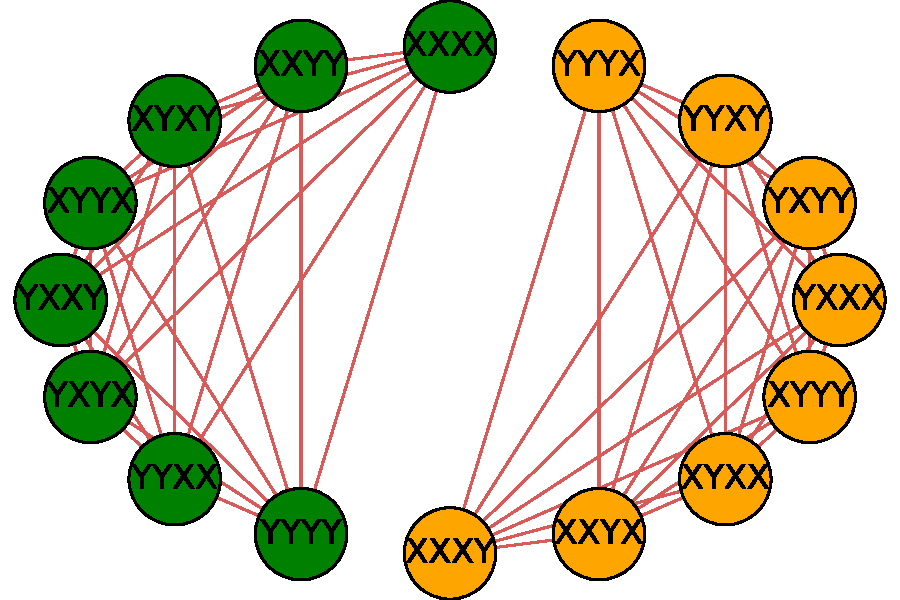
\includegraphics[width=\textwidth]{Images/JW_pqrs_term.pdf}
         \caption{Rozdělení triviálně nekomutující části Pauliho řetězců vzniklých z fermionických operátorů do dvou komutujících skupin.}
         \label{fig:Jordan_Wigner_commutation}
     \end{subfigure}
     \hfill
     \begin{subfigure}[b]{0.4\textwidth}
         \centering
         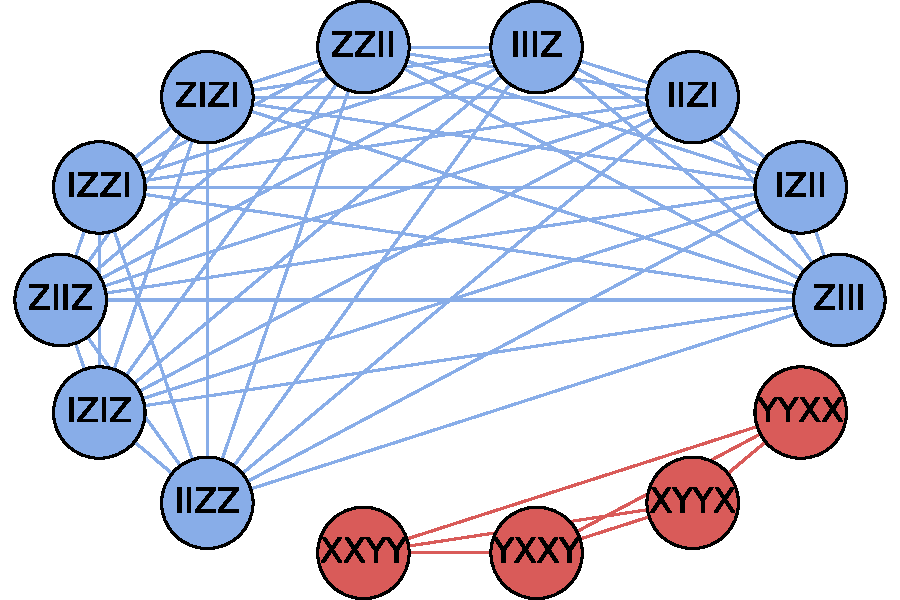
\includegraphics[width=\textwidth]{Images/H2_Full_Min_Clique_Cover.pdf}
         \caption{Ukázka rozdělení Pauliho řetězců jejichž lineární kombinace tvoří Hamiltonián molekuly LiH do komutujících skupin.}
         \label{fig:LiH_commutation_graph}
     \end{subfigure}
     \caption{Příklady rozdělení Pauliho řetězců podle komutačních vlastonstí. Převzato z \cite{gokhale_minimizing_2019}.}
\end{figure}

Počet potřebných měření lze dále snížit zaměřením se na celou sumu interakčního členu Hamiltoniánu \eqref{eq:second_quantized_hamiltonian} namísto pouze na jeden člen. Opět je BÚNO uvažováno $p>q>r>s$. 

Jak již bylo zmíněno výše, dvě disjunktní sady indexů $p,q,r,s$ generují dvě disjunktní množiny Pauliho řetězců. Navíc každý řetězec z první množiny bude komutovat s každým řetězcem z druhé množiny. To lze vypozorovat z obecného tvaru těchto řetězců \eqref{eq:pauli_a_pqrs} a relací \eqref{eq:pauli_group_relations}. Sjednocení těchto dvou množin tedy lze rozdělit na $16$ současně měřitelných množin. Navíc, jelikož lze řetězce z těchto dvou množin párovat libovolně (každý prvek z jedné komutuje s každým prvkem z druhé), je možné aplikovat výše popsanou metodu pro jednu sadu indexů a počet současně měřitelných množit tak dále zredukovat na $2$. 

Tento postup lze aplikovat i na více disjunktních sad indexů $p,q,r,s$. Například pro $16  \tfrac{N}{4}$ řetězců generovaných členy 
\begin{equation*}
    \hat a^\dag_{N} \hat a^\dag_{N-1} \hat a^{\ }_{N-2} \hat a^{\ }_{N-3}, \  \hat a^\dag_{N-4} \hat a^\dag_{N-5} \hat a^{\ }_{N-6} \hat a^{\ }_{N-7}, \ldots , \ \hat a^\dag_{4} \hat a^\dag_{3} \hat a^{\ }_{2} \hat a^{\ }_{1}
    \label{eq:a_set_1toN}
\end{equation*}
lze takto nalézt rozdělení na $16$ současně měřitelných množin, případně až na $2$ množiny při užití rozdělení pro jednu sadu indexů. Jedná se tedy o redukci o faktor $\tfrac{N}{4}$, respektive $2N$. 

Tímto způsobem lze seskupit všech $\textstyle \binom{N}{4} \approx \mathcal{O}(N^4)$ řetězců generovaných indexy $p>q>r>s$ \cite{gokhale_on3_2019}. Tyto řetězce jsou generovány různými $\tfrac{N}{4}$ prvkovými množinami $\{ \hat a^\dag_{p} \hat a^\dag_{q} \hat a^{\ }_r \hat a^{\ }_s |\, p>q>r>s \}$, kde sady indexů $p,q,r,s$ jsou disjunktní a vždy pokrývají množinu $\{ 1,2,\ldots N \}$. Tyto množiny představují obdobnou situaci jako \eqref{eq:a_set_1toN} a počet současně měřitelných skupin řetězců lze také redukovat faktorem $\tfrac{N}{4}$, respektive $2N$.

Těchto $\textstyle \binom{N}{4} \approx \mathcal{O}(N^4)$ řetězců pro $p>q>r>s$ lze tedy rozdělit na $\textstyle \binom{N}{4} / \tfrac{N}{4} \approx \mathcal{O}(N^3)$ současně měřitelných skupin. Jelikož počet řetězců pro které $p=q=r=s$ a řetězců z neinterakční části Hamiltoniánu je nižšího řádu, je tedy při užití tohoto seskupení celkový počet potřebných měření řádu $\mathcal{O}(N^3)$. 

Bylo tedy nalezeno rozdělení $\mathcal{O}(N^4)$ řetězců do $\mathcal{O}(N^3)$ současně měřitelných skupin. Nyní je ale třeba nalézt pro každou takovou množinu vhodnou bázi, ve které lze toto měření provést. Tento problém není triviální a báze mohou být tvořeny i provázanými stavy, jako v příkladu měření Pauliho řetězců v Bellově bázi výše. 

\subsection{Nalezení společné báze}

Měření jednotlivých Pauliho řetězců probíhá rotací do báze, ve které je řetězec diagonální. Tato báze je dána jako tenzorový součin bazí v nichž jsou diagonální jednotlivé Pauliho operátory tvořící řetězec. Transformace do této báze taktéž odpovídá tenzorovému součinu jednotlivých transformací pro jednotlivé Pauliho operátory, které lze nalézt v Tab. \ref{table:pauli_diagonal}, případně Tab. \ref{tab:single_qubit_conjugation}. Obdobně lze postupovat při měření množiny qubit-qubit komutujících řetězců. Tyto řetězce, jelikož pro každý index komutují, musejí mít na stejných indexech stejné Pauliho operátory nebo identitu. Tudíž lze diagonalizaci provést totožně jako pro jeden řetězec z této množiny.

Pro klasicky komutující řetězce je situace komplikovanější. Řešení lze nalézt jako postupnou aplikací transformací z tzv. \textit{Cliffordovy grupy}. Těmito unitárními transformacemi lze skupinu převést na diagonální tvar, tedy tenzorový součin operátorů $I$ a $Z$. Algoritmus kterým je tato diagonalizace implementována je obdoba Gausovské eliminace.

\textbf{Cliffordova grupa:} \textit{Cliffordova grupa} $\mathcal{C}_N$ přidružená k $\mathcal{P}_N$ je grupa unitárních transformací, které tuto grupu normalizují \cite{qubitguide}. Tedy grupa unitárních transformací $\hat U$, pro které pro libovolný Pauliho řetězec $\hat P$ z $\mathcal{P}_N$ platí:
\begin{equation}
 \hat P \in \mathcal{P}_N \implies \hat U \hat P \hat U^\dag \in \mathcal{P}_N.
\end{equation}
Prvky Cliffordovy grupy lze na kvantovém počítači implementovat pomocí tzv. \textit{Cliffordových bran}. Například brány H, S a CNOT tvoří minimální generující množinu Cliffordovy grupy. Přidáním brány T = $\sqrt{\mathrm{S}}$ = Z$^{\sfrac{1}{4}}$, která ale nepatří do Cliffordovy grupy získáme univerzální generující množinu kvantových bran.

Zajímavou podmnožinou Cliffordovy grupy jsou transformace diagonalizující Pauliho grupu. Její prvky pro $\mathcal{P}_1$ a $\mathcal{P}_2$ lze nalézt v Tab. \ref{tab:single_qubit_conjugation} respektive Tab. \ref{tab:two_qubit_conjugation}. Pomocí těchto transformací lze diagonalizovat libovolný řetězec z $\mathcal{P}_N$. Dokonce lze vhodnou aplikací diagonalizovat i libovolnou komutující množinu Pauliho řetězců, jak bude ukázáno v dále popsaném algoritmu. Nejdříve je však třeba zavést pojem \textit{stabilizační matice.}

\begin{table}[H]
\centering
\begin{tabular}{l||c|c}
      & $UZU^{\dagger}$ & $UXU^{\dagger}$ \\ \hline \hline
$U=H$ & $X$             & $Z$             \\ \hline
$U=S$ & $Z$             & $Y$            
\end{tabular}
\caption{Tabulka znázorňující prvky $\mathcal{C}_1$ diagonalizující $\mathcal{P}_1$ a jejich akci.}
\label{tab:single_qubit_conjugation}
\end{table}

\begin{table}[H]
\centering
\begin{tabular}{l||c|c|c|c}
         & $UZIU^{\dagger}$ & $UIZU^{\dagger}$ & $UXIU^{\dagger}$ & $UIXU^{\dagger}$ \\ \hline \hline
$U=CNOT$ & $ZI$             & $ZZ$              & $XX$             & $IX$             \\ \hline
$U=CZ$   & $ZI$             & $IZ$              & $XZ$             & $ZX$             \\ \hline
$U=SWAP$ & $ZI$             & $ZI$             & $IX$             & $XI$
\end{tabular}
\caption{Tabulka znázorňující prvky $\mathcal{C}_2$ diagonalizující $\mathcal{P}_2$ a jejich akci.}
\label{tab:two_qubit_conjugation}
\end{table}

\textbf{Stabilizační matice:} Pro množinu Pauliho řetězců lze zavést notaci pomocí stabilizačních matic. Řetězec o délce $N$ qubitů je reprezentován jako sloupcový vektor o $2N$ složkách. Horní $N$-tice indikuje, zda řetězec na daném indexu obsahuje operátor $\hat Z$, dolní $N$-tice zase takto enkóduje přítomnost operátoru $\hat X$. Hodnota $1$ značí přítomnost daného operátoru, hodnota $0$ zase nepřítomnost. Jelikož $\hat Y = i \hat Z \hat X \approx \hat Z \hat X$, lze operátor $\hat Y$ vyjádřit hodnotou $1$ na korespondujícím indexu pro $\hat X$ i $\hat Z$. Množinu $N$ Pauliho řetězců pak lze reprezentovat jako matici $2N$x$N$ sloučením vektorů pro jednotlivé řetězce. Tato matice se nazývá stabilizační matice. Pro množinu řetězců $\{ XXX, YYY,ZZZ,XYZ \}$ ji lze vyjádřit jako:
\begin{equation}
    \begin{pmatrix} 0 & 0 & 1 \\ 1 & 1 & 0 \\ 0 & 1 & 0 \\ 0 & 1 & 0 \\ 1 & 0 & 0 \\ 1 & 0 & 1 \end{pmatrix}
    \label{eq:stabilization_matrix}
\end{equation}

Horní část bývá nazývána $Z$-matice a spodní $X$-matice. Cílem diagonalizace je množinu komutujících řetězců převést na podmnožinu $\{ ZII\ldots I, IZI\ldots I, \ldots, III\ldots Z \}$. Pro takovou množinu bude $X$-matice bude nulová matice a $Z$ matice bude odpovídat identitě. Převod do takového tvaru lze provést obdobně jako gausovskou eliminaci, kdy řádkové úpravy budou odpovídat aplikaci Cliffordových bran z Tab. \ref{tab:single_qubit_conjugation} a Tab. \ref{tab:two_qubit_conjugation}. Jejich aplikace na všechny řetězce v množině má následující efekt na stabilizační matici \cite{aaronson_improved_2004}.
\begin{itemize}
    \item \textbf{H} aplikovaná na $i$-tý qubit prohodí $i$-tý a $(i+N)$-tý řádek matice. Tedy $\hat X$ transformuje na $\hat Z$ a naopak.
    \item  \textbf{S} aplikovaná na $i$-tý qubit vynuluje diagonální prvek $Z$-matice s indexy $i$ $i$.
    \item \textbf{CNOT} kontrolovaná $i$-tým qubitem a aplikovaná na $j$-tý qubit přičte k $i$-té řádce $j$-tou řádku a k $(j+N)$-té řádce $(i+N)$-tou. Sčítání je prováděno modulo 2.
    \item  \textbf{CZ} mezi $i$-tým a $j$-tým qubitem vynuluje prvky $Z$-matice s indexy $(i,j)$ a $(j,i)$.
    \item  \textbf{SWAP} mezi $i$-tým a $j$-tým qubitem prohodí $i$-tou a $j$-tou řádku $X$-matice i $Z$-matice.
\end{itemize}

Aplikací těchto bran tedy lze provádět řádkové úpravy a současně diagonalizovat množinu Pauliho operátorů. Zároveň je tímto postupem získán i obvod, který provádí rotaci do této nově nalezené báze. 

Ilustrujme tento postup na příkladu množiny $\{ ZII\ldots I, IZI\ldots I, \ldots, III\ldots Z \}$. Jedná se o množinu komutujících Pauliho řetězců, které však nejsou qubit-qubit komutující. Společnou měřící bázi tak získáme úpravami stabilizační matice \eqref{eq:stabilization_matrix} pro tuto množinu. Nejprve potřebujeme matici upravit tak, aby měla $X$-matice plnou hodnost. To lze tajistit aplikací Hadamardových bran. Aplikujeme tedy bránu H na první qubit. Dalším krokem je Gausovská eliminace $X$-matice. Tu lze provést prohazováním a sčítáním řádků, a tedy aplikací bran SWAP a CNOT.
 
\begin{table}[H]
\centering
%\vspace*{-\baselineskip}
\begin{tabular}{ cccc }
&\begin{quantikz}
& \gate{H} &  \\
&  &  \\
&  & 
\end{quantikz}
& $\rightarrow$ & $\begin{pmatrix} 0 & 0 & 1 \\ 1 & 1 & 0 \\ 0 & 1 & 0 \\ 0 & 1 & 0 \\ 1 & 0 & 0 \\ 1 & 0 & 1 \end{pmatrix}$ \\
\end{tabular}
\quad
\begin{tabular}{ cccc }
&\begin{quantikz}
&  &  \\
& \ctrl{1} &  \\
& \targ{} & 
\end{quantikz}
& $\rightarrow$ & $\begin{pmatrix} 0 & 0 & 1 \\ 1 & 0 & 0 \\ 0 & 1 & 0 \\
0 & 1 & 0 \\ 1 & 0 & 0 \\ 0 & 0 & 1 \end{pmatrix}$ \\
\end{tabular}
\end{table}

Nejprve přičteme druhý řádek $X$-matice k třetímu, tedy aplikujeme CNOT kontrolované druhým qubitem na třetí qubit. Dále již stačí prohodit první a druhý řádek $X$-matice a tedy aplikovat SWAP bránu na první a druý qubit. $X$-matice tak byla převedena na jednotkovou matici a $Z$-matice na symetrickou. Lze ukázat, že k této symetrizaci $Z$-matice dojde vždy. Díky ní je možno vynulovat prvky $Z$-matice pomocí S bran a CZ bran. S brány vynulují diagonální elementy a CZ zase mimodiagonální elementy. Aplikujeme tedy na první qubit S bránu a na druhý a třetí CZ bránu. $X$-matici tyto brány neovlivní.

\begin{table}[H]
\centering
%\vspace*{-\baselineskip}
\begin{tabular}{ cccc }
&\begin{quantikz}
& \swap{1} &  \\
&  \targX{} &  \\
&  & 
\end{quantikz}
& $\rightarrow$ & $\begin{pmatrix} 1 & 0 & 0 \\ 0 & 0 & 1 \\ 0 & 1 & 0 \\
1 & 0 & 0 \\ 0 & 1 & 0 \\ 0 & 0 & 1 \end{pmatrix}$ \\
\end{tabular}
\quad
\begin{tabular}{ cccc }
&\begin{quantikz}
& \gate{S} &  \\
& \ctrl{1} &  \\
& \control{} & 
\end{quantikz}
& $\rightarrow$ & $\begin{pmatrix} 0 & 0 & 0 \\ 0 & 0 & 0 \\ 0 & 0 & 0 \\
1 & 0 & 0 \\ 0 & 1 & 0 \\ 0 & 0 & 1 \end{pmatrix}$ \\
\end{tabular}
\end{table}

Nyní máme $X$-matici ve tvaru jednotkové matice a $Z$-matici nulovou. Požadujeme však přesný opak. Toho lze dosáhnout aplikací H na všechny qubity.

\begin{table}[H]
\centering
%\vspace*{-\baselineskip}
\begin{tabular}{ cccc }
&\begin{quantikz}
& \gate{H} &  \\
&  \gate{H} &  \\
& \gate{H} & 
\end{quantikz}
& $\rightarrow$ & $\begin{pmatrix} 1 & 0 & 0 \\ 0 & 1 & 0 \\ 0 & 0 & 1 \\
0 & 0 & 0 \\ 0 & 0 & 0 \\ 0 & 0 & 0 \end{pmatrix}$ \\
\end{tabular}
\end{table}

Nalezli jsme tedy společnou bázi Pauliho řetězců, ve které jsou diagonální. Obvod, který provede transformaci stavu do této báze má tvar Obr. \ref{fig:stabilization_diagonalization_example}. SWAP brána v tomto obvodu může být vynechána a namísto toho implementována jako prohození následujících bran s prohozením indexů příslušných qubitů při měření. 

\begin{figure}
    \centering
\begin{table}[H]
\centering
%\vspace*{-\baselineskip}
\begin{tabular}{ ccccc }

$\begin{pmatrix}
0 & 1 & 0 \\ 1 & 1 & 0 \\ 0 & 1 & 0 \\
0 & 0 & 1 \\ 1 & 0 & 0 \\ 1 & 0 & 1\end{pmatrix}$ & $\rightarrow$ & 
\begin{quantikz}
    & \gate{H} & \swap{1} & \gate{S}   & \gate{H} & \\
    & \ctrl{1} & \targX{} & \ctrl{1}   & \gate{H} & \\
    & \targ{} &           & \control{} & \gate{H} &
\end{quantikz}
& $\rightarrow$ & $\begin{pmatrix}
1 & 0 & 0 \\ 0 & 1 & 0 \\ 0 & 0 & 1 \\
0 & 0 & 0 \\ 0 & 0 & 0 \\ 0 & 0 & 0
\end{pmatrix}$ \\
\end{tabular}
\end{table}
    \caption{Ukázka diagonalizace množiny Pauliho operátorů u reprezentaci pomocí stabilizační matice a příslušného vantového obvodu pro tuto diagonalizaci.}
    \label{fig:stabilization_diagonalization_example}
\end{figure}

Obecně lze tento postup realizovat pomocí Algoritmu \ref{alg:circuit_synthesis} převzaného z \cite{gokhale_minimizing_2019}. Klasická náročnost algoritmu pro pro $N$ řetězců o délce $N$ bude odpovídat nejnáročnějšímu kroku, a tedy Gausově eliminaci, která má náročnost řádu $\mathcal{O}(N^3)$. Gausovská eliminace vyžaduje maximálně $\mathcal{O}(N^2)$ řádkových operací, což odpovídá aplikaci $\mathcal{O}(N^2)$ kvantových bran. Vynulování prvků $Z$-matice pomocí S a CZ bran vyžaduje také $\mathcal{O}(N^2)$ bran. Celkově tak měření množiny klasicky komutujících Pauliho řetězců vyžaduje dodatečnou aplikaci obvodu čítajícího $\mathcal{O}(N^2)$ bran. To se může zdát jako nevýhoda oproti měření řetězců po jednom nebo měření qubit-qubit komutující skupiny, které obojí vyžadují pouze $\mathcal{O}(N)$ bran. Příprava stavu však vyžaduje, jak bude naznačeno dále v části rozebírající ansatz pro VQE, počet bran řádu většího, než $\mathcal{O}(N^2)$. Počet bran aplikovaných dodatečne, pro rotaci stavu do měřící báze je tedy zanedbatelný. Hlavní výhoda seskupování Pauliho řetězců netkví v redukci počtu bran nutného k přípravě stavu, nýbrž v redukci počtu stavů, které je třeba připravit. Postupy, které byly popsány v této části umožňují redukci z $\mathcal{O}(N^4)$ potřebných příprav až na $\mathcal{O}(N^3)$.

\begin{algorithm}
\SetAlgoLined
\SetKwInOut{Input}{input}\SetKwInOut{Output}{output}
\Input{ $\{P_i\}$, a complete GC family of Pauli strings}
\Output{ Circuit for simultaneous measurement of $\{P_i\}$}
\BlankLine
$M \in F_2^{2N \times N} \leftarrow$ basis of $\{P_i\}$\;
Full-rankify $Z$-matrix by applying $H$ gates\;
Gaussian eliminate $X$-matrix using CNOT \& SWAP gates\;
\For{each diagonal element in $Z$-matrix}{
\lIf{element is 1}{apply $S$ to corresponding qubit}
}
\For{each element below diagonal of $Z$-matrix}{
\lIf{element is 1}{apply $CZ$ to the row-col qubits}
}
Apply $H$ to each qubit\;
Measure each qubit\;
\caption{Algoritmus k nalezení obvodu pro transformaci stavu do měřící báze pro množinu Pauliho řetězců. Převzato z \cite{gokhale_minimizing_2019}.}
\label{alg:circuit_synthesis}
\end{algorithm}


\section{Ansatz}
Základní myšlenkou VQE je postupné procházení Hilbertova prostoru Hamiltoniánu a hledání minima jeho střední hodnoty. Parametrizovaný kvantový obvod, který vytváří stavy aproximující tento prostor bývá nazýván \textit{ansatz}. Ansatzem také často bývá nazýván parametrizovaný unitární operátor reprezentovatelný na kvantovém počítači, který svou aplikací na nějaký výchozí stav vytváří kýžené parametrizované stavy. Cílem ansatzu tedy je připravit stav
\begin{equation}
    \kett{\psi(\vec \theta)} = \hat U (\vec \theta) \ket{\psi_0},
\end{equation}
který umožňuje volbou parametrů $\vec \theta$ aproximovat vlastní stavy Hamiltoniánu. Výběr ansatzu je jedním z hlavních stavebních kamenů VQE. Nalezení efektivního ansatzu předtavuje hledání kompromisu mezi pokrytím Hilbertova prostoru daného problému a trénovatelností obvodu. S pokrytím stavů systému roste počet parametrů ansatzu a také počet iterací potřebných k dosažení konvergence při hledání minima a tedy klesá trénovatelnost. V praxi tak bývá zvykem omezit se pokrytím na menší podprostor, tento podprostor ale musí obsahovat a dobře popisovat hledaný základní stav a jeho okolí, aby byla zachována trénovatelnost. Zvykem bývá omezit pokrytí ansatzu pouze na prostor několika stavů s nejnižšími energiemi. 

Trénovatelnost značně souvisí s problémem tzv. \textit{barren plateau} \cite{mcclean_barren_2018}, v doslovném překladu problém nehostinných náhorních plošin. Jedná se o problém exponenciálně se zmenšujícího se gradientu optimalizační krajiny při hledání minima. V analogii optimalizační krajiny s reálnou třídimenzionální krajinou je pak původ názvu očividný. Lze snadno nahlédnout, proč toto představuje pro VQE problém. Měření stavu je stochastický problém, jehož přesnost je tím pádem dána počtem opakování (výstřelů). Optimalizace ve VQE obvykle vyžaduje aproximaci gradientu pro určení parametrů pro další iteraci, gradient bývá aproximován pomocí měření pro několik různých hodnot optimalizačních parametrů. Zmenšuje-li se však gradient exponenciálně, rostou exponenciálně nároky na přesnost a tedy i počet měření. V extrémních případech může mít tento efekt za následek nemožnost spočítat gradient s dostatečnou přesností v rozumné čase a znemožní tak další úspěšnou optimalizaci a konvergenci VQE.

Problém může být potlačen vhodnou volbou ansatzu. Ukazuje se například, že restrikce pokrytí ansatzu pouze na část Hilbertova prostoru má na problém náhorních plošin pozitivní efekt \cite{holmes_connecting_2022} \cite{mcclean_barren_2018}. Problém lze také potlačit volbou, či modifikací optimalizační strategie \cite{haug_optimal_2021}.

Ansatzy lze také rozdělit podle motivace k danému tvaru obvodu. Dvěma nejzastoupenějšími kategoriemi jsou \textit{hardwarově motivoané ansatzy (HEA)} a \textit{fyzikálně motivované ansatzy}. Nejpoužívanějším fyzikálně motivovaným ansatzem je \textit{Unitary coupled cluster (UCC)}, který vychází z \textit{Coupled cluster} (CC) teorie. 

\subsection{HEA}
Hardwarově motivované ansatzy jsou specificky navržené tak, aby je bylo možné efektivně realizovat na příslušném kvantovém počítači. Jsou tedy velice specifické, avšak vycházejí z podobných principů. Cílem ansatzu je vytvořit provázané parametrizované stavy. V HEA toho bývá docíleno aplikací jednoqubitových parametrizovaných rotačních bran a vícequbitových bran vytvářejících provázání. Tyto brány jsou pak uspořádány do bloků, ze kterých je ansatz sestaven. Příkladem bran, které bývají ke konstrukci takového ansatzu užity jsou například parametrizované rotační brány R$_x(\theta)$, R$_y(\theta)$ a CNOT.

\subsection{Unitary Coupled Cluster}
\textit{Unitary coupled cluster} je metoda vyvinutá původně na aproximaci elektronových vlnových funkcí v molekulách a atomech, ve výpočetní chemii se stala standardem \cite{anand_quantum_2022}. Nachází však uplatnění například i ve fyzice atomového jádra \cite{bhoy_shell-model_2024}, či vnitřní struktury hadronů \cite{gallimore_quantum_2023}. Jedná se o unitární variantu \textit{Coupled cluster (CC)} metody. 

\textbf{Coupled cluster:} CC je metoda umožňující konstruovat vícečásticové vlnové funkce aplikací excitačních operátorů na vlnovou funkci popisující jednočásticový orbital. Tím vytváří lineární kombinace jednočásticových excitovaných stavů. O rozvoj CC se mimo jiné zasloužil také Český chemik Jiří Čížek \cite{cizek_correlation_1966}. 

Vlnová funkce v CC metodě má podobu
\begin{equation}
    \ket{\psi_\mathrm{CC}} = \mathrm{e}^{\hat T} \ket{\psi_0},
\end{equation}
kde stav $\ket{\psi_0}$ je stav se zaplněným pouze okupačním číslem s nejnižší energií. Ačkoliv má takový stav nejnižší energii pouze v prostoru jednočásticových stavů, může být považován za aproximaci základního stavu systému. Operátor $\hat T$ se nazývá excitační operátor a lze jej vyjádřit jako superpozici jednoduchého excitačního operátoru $\hat T_1$, dvojitého excitačního operátoru $\hat T_2$, až $n$-násobného excitačního operátoru: 

\begin{align} \begin{split}
    \hat T \, & = \hat T_1 + \hat T_2 + \hat T_3 + \ldots \\ 
    \hat T_1 &= \sum_{ia} \theta_i^a \hat a_a^\dag \hat a^{\,}_i \\
    \hat T_2 &= \sum_{ijab} \theta_{ij}^{ab} \hat a_a^\dag \hat a_b^\dag \hat a^{\,}_i \hat a^{\,}_j \\
    & \ \ \vdots
    \label{eq:excitacni_operatry}
    \end{split}
\end{align}

Indexy $i,j$ číslují obsazené orbitaly a indexy $a,b$ neobsazené (virtuální) orbitaly. Varianty CC bývají často nazývány podle řádu excitací, které zahrnují. Tedy například CCS (Coupled cluster single) zahrnuje pouze jednoduché (single) excitace a CCSD (Coupled cluster single double) zahrnuje i dvojité excitace. Operátor $\mathrm{e}^{\hat T}$ není unitární a proto jej nelze přímo implementovat na kvantovém počítači. Operátor $\hat T$ je totiž Hermitovský a tudíž jeho exponenciála není unitární. 

\textbf{Unitary coupled cluster:} Tento problém řeší \textit{Unitary coupled cluster (UCC)}. Jeho přehlednou formulaci, možné modifikace a aplikace lze nalézt například v souhrnném článku \cite{anand_quantum_2022}. Aby byla exponenciála operátoru unitární, musí být tento operátor anti-Hermitovský. UCC proto zavádí operátor $\hat T - \hat T^\dag$, který je dán rozdílem excitačního a deexcitačního operátoru a je anti-Hermitovský. Jeho exponenciála tak bude unitární operátor a pro UCC ansatz lze psát:
\begin{equation}
    \ket{\psi_\mathrm{UCC}} = \mathrm{e}^{\hat T - \hat T^\dag} \ket{\psi_0}.
\end{equation}
Tento unitární operátor již lze implementovat na kvantovém počítači. Excitační operátory v exponenciále nekomutují a tudíž nemůže být suma rozložena na součin exponenciál jednotlivých členů \cite{modra_smrt}. Tento problém je řešen aproximací nazývanou \textit{Trotteizace} nebo také \textit{Trotter-Suzuki dekompozice.}

\textbf{Troterizace:} Tuto aproximaci lze získat aplikací Taylorova rozvoje a binomické věty. V prvním řádu má tvar:
\begin{equation}
    \mathrm{e}^{\hat T - \hat T^\dag} = \mathrm{e}^{\sum_i \theta_i (\hat T_i - \hat T_i^\dag) } \approx \left ( \prod_i \exp ({\tfrac{\theta_i}{t} (\hat T_i - \hat T_i^\dag) } ) \right )^t + \mathcal{O}(\tfrac{1}{t}),
\end{equation}
kde $t$ je Trotterovo číslo a bývá často položeno rovno $1$ a rozklad tak odpovídá rozkladu pro exponenciálu komutujících operátorů. Ansatz pro UCC tak lze v této aproximaci psát jako:
\begin{equation}
    \kett{\psi_\mathrm{UCC}(\vec \theta)} = \hat U (\vec \theta) \ket{\psi_0} \approx  \prod_{i=1}^n \mathrm{e}^{ \theta_i \, (\hat T^{\,}_i - \hat T_{\, i}^\dag)} \ket{\psi_0},
\end{equation}
kde $n$ je nejvyšší řád možné excitace. Tedy například pro $n=2$ jsou uvažovány pouze jednoduché a dvojité excitace a ansatz pak bývá nazýván UCCSD ansatz (UCC Single Double). Dále $\theta_i$ představují trénovatelné parametry jejichž variací je procházen stavový prostor.

Takto vytvořený ansatz je třeba implementovat jako obvod na kvantovém počítači. Anihilační a kreační operátory v excitačních operátorech \eqref{eq:excitacni_operatry} lze vyjádřit pomocí Pauliho řetězců jako v případě reprezentace Hamiltoniánu v předchozích sekcích. Lze užít například Jordan-Wigner transformaci \eqref{eq:Jordan_Wigner}, paritní enkódování nebo Bravyi-Kitaev transformaci. Ansatz pak bude mít podobu součinu exponenciál Pauliho řetězců přenásobených parametry $\theta$. Takové exponenciály lze převést do podoby kvantového obvodu tzv. \textit{Schodišťovým algoritmem}.

\textbf{Schodišťový algoritmus:} Cílem schodišťového algoritmu je vyjádřit operátory typu
\begin{equation}
    \hat U = \mathrm{e}^{i\tfrac{\theta}{2} \hat P_n},
\end{equation}
kde $P_n$ je Pauliho řetězec z $\mathcal{P}_n$ a faktor $\tfrac{1}{2}$ je zvolen z důvodu přehlednosti výsledného obvodu. Algoritmus lze nalézt přehleně popsaný například v \cite{mansky_decomposition_2023}. Základním stavebním kamenem metody je obvod pro exponenciálu řetězce $\hat Z \otimes \hat Z$, tedy operátor $\mathrm{e^{i\tfrac{\theta}{2} \hat Z \otimes \, \hat Z}}$. Ten je tvořen bránou $R_z(\theta)$ obloženou dvěma CNOT a lze jej nalézt na Obr. \ref{fig:expZZ}.

\begin{figure}[H]
    \centering
    \begin{quantikz}
        & \ctrl{1} & & \ctrl{1} & \\
        & \targ{} & \gate{R_z(\theta)} & \targ{} &
    \end{quantikz}
    \caption{Implementace operátoru $\exp (i \tfrac{\theta}{2} \hat Z_1 \hat Z_2)$ pomocí kvantového obvodu.}
    \label{fig:expZZ}
\end{figure}

To, že obvod opravdu odpovídá exponenciále řetězce $\hat Z \hat Z$ lze snadno ověřit užitím následující identity pro CNOT:
\begin{equation}
    CNOT = \p{0} \otimes \hat I + \p{1} \otimes \hat X
\end{equation}
a následujícího rozpisu, který lze získat z Taylorova rozvoje pro exponenciálu a goniometrické funkce:
\begin{equation}
    \mathrm{e^{i\tfrac{\theta}{2} \hat Z \otimes \, \hat Z}} = \cos \tfrac{\theta}{2} \hat I_1 \otimes \hat I_2 - i \sin \tfrac{\theta}{2} \hat Z_1 \otimes \hat Z_2.
\end{equation}
Dále lze z těchto identit a vztahů mezi Pauliho operátory, viz Tab. \ref{tab:single_qubit_conjugation} nebo Tab. \ref{table:pauli_diagonal}, odvodit, že působí-li v exponenciále na některý qubit operátor $\hat X$, stačí do obvodu přidat dvojici Hadamardových bran $\hat H$ aplikované na příslušný qubit. Obdobně pro operátor $\hat Y$ je nutno přidat bránu $R_x(\tfrac{\pi}{2})$ odpovídající součinu bran S a H. 
Jedná se o případ obdobný měření Pauliho operátorů, kde bylo třeba operátory $\hat X$ a $\hat Y$ převést do $Z$-báze stejnými transformacemi. Příklad rozkladu takových exponenciál do kvantového obvodu lze nalézt na Obr. \ref{fig:XZ_and_ZY}.

\begin{figure}[H] 
     \centering
     \begin{subfigure}[b]{0.45\textwidth}
         \centering
            \begin{quantikz}
               &\gate{H} & \ctrl{1} & & \ctrl{1} & \gate{H} & \\ 
                && \targ{} & \gate{ R_z (\theta) } & \targ{} &&
            \end{quantikz}
         \caption{$\hat X \otimes \hat Z$}
         \label{fig:expXZ}
     \end{subfigure}
     \begin{subfigure}[b]{0.5\textwidth}
         \centering
            \begin{quantikz}
                &  \ghost{H} & \ctrl{1} & & \ctrl{1} &  & \\
                &\gate{R_x(\tfrac{\pi}{2})} & \targ{} & \gate{ R_z (\theta) } & \targ{} &\gate{R_x(-\tfrac{\pi}{2})}&
            \end{quantikz}
         \caption{$\hat Z \otimes \hat Y$}
         \label{fig:expZY}
     \end{subfigure}
        \caption{Implementace operátorů $\mathrm{e^{i\tfrac{\theta}{2} \hat X \otimes \, \hat Z}}$ a $\mathrm{\, e^{i\tfrac{\theta}{2} \hat Z \otimes \, \hat Y}}$ na kvantovém počítači. Od implementace exponenciály $\hat Z \otimes \hat Z$ z Obr. \ref{fig:expZZ} se liší přidáním páru jednoqubitových bran.}
        \label{fig:XZ_and_ZY} 
\end{figure}

Základ obvodu tedy vždy tvoří brána $R_Z(\theta)$ obložená dvěma CNOT, tedy obvod na Obr. \ref{fig:expZZ}. Přidání každého dalšího Pauliho operátoru v exponenciále koresponduje v obvodu s přidáním qubitu a párem CNOT bran přidaných z vnější strany původního obvodu. Obvod tak má podobu "schodiště" budovaného pomocí CNOT. Působí-li na některý qubit v exponenciále jiný Pauliho operátor než $\hat Z$, postačí příslušný qubit v obvodu obložit dvojicí bran odpovídající transformaci mezi tímto Pauliho operátorem a $\hat Z$. Například obvod pro exponenciálu řetězce $\hat X \otimes \hat Y \otimes \hat Z$ bude odpovídat tvaru na Obr. \ref{fig:expXYZ}. 


\begin{figure}[H]
    \centering
    \begin{quantikz}
        & \gate{H} & \ctrl{1} &      &     &  & \ctrl{1} & \gate{H} & \\
        & \gate{R_z(\tfrac{\pi}{2})} &\targ{} & \ctrl{1} & & \ctrl{1} & \targ{} & \gate{R_z(-\tfrac{\pi}{2})} & \\
        &&          & \targ{}  & \gate{R_z (\theta)} & \targ{}  &          &&
    \end{quantikz}
    \caption{Implementace operátoru $\exp (i \tfrac{\theta}{2} \hat X \hat Y \hat Z)$ pomocí kvantového obvodu. Za každý další operátor v Pauliho řetězci je přidán pár CNOT a případně pár jednoqubitových bran příslušejících danému operátoru.}
    \label{fig:expXYZ}
\end{figure}

Identitu v Pauliho řetězci v exponenciále lze v obvodu realizovat pomocí dvojice SWAP bran, opět aplikovaných z vnějšku. Alternativně lze příslušný qubit ponechat beze změny. Obě možnosti jsou znázorněny na Obr. \ref{fig:exp_identita}.

\begin{figure}[H]
     \centering
     \begin{subfigure}[b]{0.45\textwidth}
         \centering
            \begin{quantikz}
                & \ctrl{1} &      &     &  & \ctrl{1} & \\
                &  \targ{} & \swap{1} & & \swap{1} & \targ{} &  \\
                &          & \targX{}  & \gate{R_z (\theta)} & \targX{}  & &
            \end{quantikz}
         \caption{Implementace užitím páru SWAP bran. \vspace{.3cm}}
         \label{fig:expXI_swap}
     \end{subfigure}
     \begin{subfigure}[b]{0.45\textwidth}
         \centering
            \begin{quantikz}
                & \ctrl{1} &      &     &  & \ctrl{1} & \\
                &  \targ{} &  & \gate{R_z (\theta)} & & \targ{} &  \\
                &          &   &  &   & &
            \end{quantikz}
         \caption{Je-li $\hat I$ aplikováno na některý z krajních qubitů, lze SWAP brány kompletně vynechat a s daným qubitem nijak nemanipulovat.}
         \label{fig:expXI}
     \end{subfigure}
        \caption{Implementace exponenciály Pauliho řetězce, který obsahuje $\hat I$.}
        \label{fig:exp_identita}
\end{figure}

UCC ansatz tedy lze pomocí některé z fermion-qubit transformací převést na součin exponenciál Pauliho řetězců. Tyto exponenciály jednotlivých řetězců pak lze vyjádřit pomocí těchto jednoduchých bloků a tak složit celý obvod pro UCC.

\section{Optimizéry}
Z klasického pohledu je VQE úloha na hledání extrému funkce více proměnných. Funkce $C(\vec \theta)$, která je optimalizovaná bývá nazývána \textit{Cost funkce}. VQE tak lze formulovat jako:

\begin{equation}
\min_{\vec\theta} C(\vec\theta) = 
\min_{\vec\theta} \langle \psi(\vec\theta)|\hat{\mathcal{H}}|\psi(\vec\theta)\rangle.
\end{equation}

Případně lze také VQE formulovat pomocí pseudokódu jako algoritmus \ref{alg:vqe}.


\begin{algorithm}
\SetAlgoLined
\KwResult{Přibližná energie základního stavu, $\min_{\vec{\theta}} \langle \psi(\vec\theta)| \hat H |\psi(\vec\theta)\rangle$ } 
$\vec{\theta_0} \ - \ $ náhodně incializované úhly\;
$i = 0$\;
\While{není dosažena konvergence}{
  \For{$j \in [O(N^4)]$}{
    \For{$O(1/\epsilon^2)$ opakování}{
    Připrav stav $\ket{\psi(\vec \theta_i)}$\;
    Změř $\langle \psi(\vec\theta_i)| \hat H_j |\psi(\vec\theta_i)\rangle$\;
    }
  }
  $\langle \psi(\vec\theta)| \hat H |\psi(\vec\theta)\rangle = \sum_j \langle \psi(\vec\theta_i)| \hat H_j |\psi(\vec\theta_i)\rangle $ \;
  $i$++\;
Urči nové $ \vec \theta_i$ pomocí optimizéru\;

 }
 \caption{Variational Quantum Eigensolver (VQE)}
 \label{alg:vqe}
\end{algorithm}

Optimalizace probíhá na klasickém počítači. Část výpočtu cost funkce však probíhá na kvantovém počítači, musí proto být pro hledání minima použit algoritmus, který nezávisí na tom, jakým způsobem je hodnota cost funkce získána.
Algoritmy hledající iterativně extrém funkce bývají nazývány \textit{optimizéry}. Lze je rozdělit do dvou kategorií, \textit{gradientní} a \textit{negradientní}. Tedy metody, které k určení parametrů pro další iteraci využívají gradient a metody které určují parametry jiným způsobem. Srovnání nejpoužívanějších optimizérů pro účely VQE lze nalézt například v \cite{bonet-monroig_performance_2023}, pro použití v algoritmu VQLS, podobnému VQE zase například v \cite{pellow-jarman_comparison_2021}. V této části jich bude několik stručně popsáno.


\subsection{Gradientní Optimizéry}
Optimizéry využívající gradient jsou velice populárními optimizéry, které v posledních letech prošly značným vývojem. Důvodem je \textit{hluboké učení} (de facto trénování neuronových sítí), kde je využíván výhradně tento typ optimizérů \cite{aggarwal_neural_2023}. Tyto algoritmy jsou často modifikací, či rozšířením algoritmu známého jako \textit{gradient descent}, který iterativně odčítá gradient od odhadu souřadnic minima a tím tento odhad zpřesňuje. K úspěšné aplikaci těchto metod je však třeba znát gradient cost funkce, kterou optimalizujeme.

\textbf{Výpočet gradientu:} Jelikož část výpočtu cost funkce je realizována kvantovým počítačem, není možné gradient určit přímo klasickým analytickým přístupem. Tento problém řeší metody umožňující aproximovat gradient pomocí hodnoty funkce v několika bodech. Dvě nejpoužívanější žpůsoby pro aproximaci gradientu cost funkce jsou \textit{metoda konečných diferencí} a metoda \textit{SPSA}.

\begin{itemize}
    \item Aproximace pomocí \textit{konečných diferencí (FD - finite differences)} patří k nejjednodušším metodám pro odhad gradientu. Každou složku gradientu vyjádří jako diferenci danou posunutím ve směru daném jednotkovým vektorem příslušné složky. Pro $j$-tou složku gradientu, která představuje derivaci podle parametru $\theta_j$ lze vyjádřit jako rozdíl funkčních hodnot $C(\vec \theta)$ posunutých o hodnotu $\pm c_n$ ve směru $j$-tého souřadnicového vektoru normovanoý velikostí tohoto posunutí. Tedy pro $j$-to složku gradientu v $n$-té iteraci platí:
\begin{equation}
    (g(\vec \theta_n))_j = \frac{C(\vec \theta - c_n \vec e_j) - C(\vec \theta + c_n \vec e_j)}{2c_n},
\end{equation}
kde $\vec \theta_n$ je $n$-tý odhad parametrů $\vec \theta$ a hodnota $c_n$ je obvykle snižována s počtem provedených iterací $n$. Pro každou složku gradientu je třeba tedy provést $2$ ohodnocení funkce. Má-li vektor parametrů $p$ složek, pak má $p$ složek i gradient a k jeho aproximaci je tak třeba $2p$ ohodnocení funkce.
\item \textit{Simultaneous perturbation stochastic approximation (SPSA)} je metoda umožňující aproximovat gradient pomocí menšího počtu ohodnocení funkce. Gradient je vypočten jako diference funkční hodnoty ve dvou bodech získaných náhodnou perturbací $\vec \delta$. V $n$-té iteraci má tak $j$-tá složka gradientu tvar:
\begin{equation}
    (g(\vec \theta_n))_j = \frac{C(\vec \theta - c_n \vec \delta_n ) - C(\vec \theta + c_n \vec \delta_n)}{2c_n (\delta_n)_j}.
\end{equation}
Tato metoda, na rozdíl od konečných diferencí vyžaduje pouze dvě ohodnocení funkce k určení celého gradientu, nikoliv jen jedné jeho složky. Náhodná inicializace perturbačního vektoru $\vec \delta$ také přispívá k rezistenci metody vůči náhodnému šumu \cite{tilly_variational_2022}.
\item Další, avšak ne tolik používanou možností je gradient určit analyticky přímo na kvantovém počítači. Tato metoda využívá tzv. \textit{parameter shift rules}, které umožňují výpočet parciálních derivací. Tato metoda byla poprvé navržena pro účely kvantového strojového učení v \cite{mitarai_quantum_2018} a dále rozvinuta v \cite{schuld_evaluating_2019}. Metoda využívá toho, že ansatz má podobu exponenciály, jejíž derivace odpovídá pouze přenásobení konstantou v argumentu. V ansatzu má tato konstanta podobu Pauliho řetězce, a tak parciální derivace podle parametru $\theta_i$ odpovídá vložení správného Pauliho řetězce do ansatzu.
\end{itemize}

\textbf{Gradient descent:} Počátek klasické verze tohoto algoritmu se datuje až do první poloviny $19$. století k Francouzskému mataematikovi A.L. Cauchymu \cite{cauchy_analyse_2009}. Lze jej rekurzivně popsat následujícím způsobem: 
\begin{equation}
    \vec \theta_{n+1} = \vec \theta_n - \eta \, \vec g(\vec \theta_n),
    \label{eq:gradient_descent}
\end{equation}
kde $\vec \theta_i$ je odhad parametrů v minimu, $\vec g_n = \vec g(\vec \theta_n)$ je gradient optimalizované funkce určený pro sadu parametrů $\vec \theta_n$ a parametr $\eta$ nazývaný \textit{learing rate} škálující gradient před jeho odečtením. 

Vývoj v posledních letech, spojený s hlubokým učením měl za následek postupné modifikace algoritmu za účelem eliminace některých problémů. Přehled nejpopulárnějších rozšíření lze nalézt například v článku \cite{ruder_overview_2017}. Nejpoužívanější variantou ve VQE je modifikace nazývaná \textit{Adam}. Adam je založen na principech modifikací \textit{Momentum}, \textit{Adagrad} a \textit{Adadelta}, a proto budou nejprve popsány tyto optimizéry.

\textbf{Momentum:} Tento optimizér navržen \cite{qian_momentum_1999} k potlačení problému, kdy optimalizace konvergovala do lokálního minima, či kolem něj oscilovala. Gradient z předchozích iterací je akumulován, a každá iterace je tak ovlivněna těmi předchozími. Název algoritmu pochází z analogie s fyzikálním problémem balvanu kutálejícího se z kopce. Takový balvan postupně akumuluje hybnost a narazí-li na lokální minimum, je ho schopen za ztráty části naakumulované hybnosti překonat a pokračovat dále, až do údolí, kde zasáhne nic netušícího turistu. Tento algoritmus lze rekurzivně vyjádřit jako následujícím způsobem:

\begin{equation} \begin{split}
\vec v_n \ &= \gamma \, \vec v_{n-1} + \eta \, \vec g(\vec \theta_n) \\
\vec \theta_{n+1} &= \vec \theta_n - \vec v_n.
\end{split} \end{equation}
Parametry pro další iteraci jsou tedy určeny odečítáním vektoru $\vec v_n$, který kromě gradientu vyčísleného pro aktuální parametry zahrnuje i část vektoru $\vec v$ z předchozí iterace. To, jakou vahou předchozí iterace přispívají je dáno parametrem $\gamma$.

\textbf{Adagrad:} Optimizér navržený v \cite{adagrad} implementuje proměnný learning rate. Každý parametr ze sady $\vec \theta$ je tak optimalizován v jiné míře. Prioritizována je aktualizace méně se měnících parametrů a naopak potlačena aktualizace těch více proměnných. Tohoto efektu je dosaženo tak, že je learning rate pro $j$-tý parametr $\theta_j$ normován součtem kvadrátů $j$-tých složek gradientů z předchozích iterací. Rekurzivně lze pak pro $j$-tý parametr v $n$-té iteraci $\theta_{n,j}$ psát:

\begin{equation} \begin{split}
    G_{n,j} &= \sum_{i=1}^n g^2_{i,j} \\
    \theta_{n+1,j} &= \theta_{n,j} - \frac{\eta}{\sqrt{G_{n,j} + \epsilon}} g_{n,j},
\end{split} \end{equation}
kde $g_{n,j}$ představuje $j$-tou složku gradientu vyčíslenou pro hodnoty parametrů $\theta$ z $n$-té iterace a $\epsilon$ je malá konstanta zabraňující dělení nulou. 

\textbf{Adadelta:} Adagrad má za následek agresivní útlum learning rate parametru. Tento problém řeší rozšíření tohoto optimizéru, optimizér adadelta nevržený v \cite{zeiler2012adadeltaadaptivelearningrate}. Learning rate je zde, namísto součtu kvadrátu všech předchozích gradientů normován klouzavým průměrem gradientů. Tento klouzavý průměr $E[g^2]_n$ závisí pouze na klouzavém průměru předchozí iterace a gradientu vyčísleném pro parametry z aktuální iterace. Rekurzivní zápis tohoto optimizéru je

\begin{equation} \begin{split}
E[g^2]_n &= \gamma \, E[g^2]_{n-1} + (1-\gamma) g^2_n \\
    \vec \theta_{n+1} &= \vec \theta_n - \frac{\eta}{\sqrt{E[g^2]_n + \epsilon} } \vec g_n.
\end{split} \end{equation}

\textbf{Adam:} Adaptive Moment Estimation, zkráceně Adam navržený v \cite{kingma_adam_2017} je kombinací výše popsaných optimizérů. Zahrnuje proměnný learning rate realizovaný pomocí klouzavého průměru druhé mocniny gradientu i akumulaci gradientů z předchozích iterací jako v optimizéru mommentum. Kromě parametru $\eta$ jsou zde ještě parametry $\beta_1$ a $\beta_2$ ovlivňující, jak moc se předchozí iterace promítají do dalšího průběhu optimalizace. Adam lze zapsat jako:

\begin{align} \begin{split}
    \vec m_n &= \beta_1 \vec m_{n-1} + (1 - \beta_1) \vec g_n \\
      v_n \  &= \beta_2 v_{n-1}  + (1-\beta_2) g^2_n \\
    \vec \theta_{n+1} &= \vec \theta_n  - \frac{\eta}{\sqrt{v_n} + \epsilon} \vec m_n.
\end{split} \end{align}
Průměrování gradientů v členech $v_n$ a $\vec m_n$ zlepšují rezistenci optimizéru vůči šumu, tudíž může být dobře aplikován pro účely VQE.

\subsection{Negradientní}

\textbf{Nelder-Mead:}
-Nelder-Mead \cite{nelder_simplex_1965} vizualizace \cite{dowad_visualizing_nodate}

\begin{figure}[H]
    \centering
    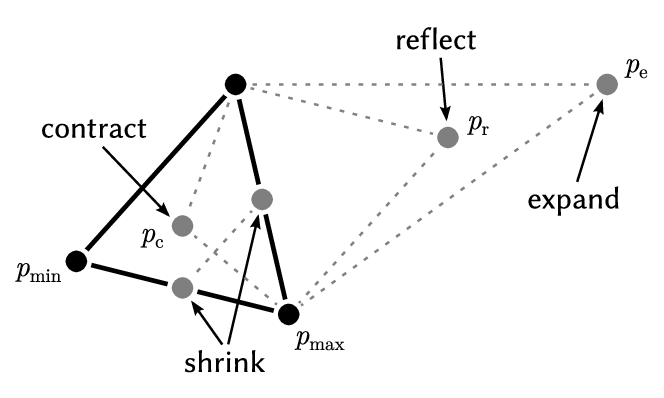
\includegraphics[width=0.5\linewidth]{Images/Nelder_mead.png}
    \caption{Ukázka Nelder-Mead algoritmu v rovině. Převzato z \cite{CHENG201580}.}
    \label{fig:Nelder_Mead}
\end{figure}

\textbf{Powel:}
Powel \cite{powell_efficient_1964}

\textbf{COBYLA:}
Constrained Optimization BY Linear Approximation (COBYLA) \cite{Powell_cobyla}

\textbf{Rotosolve:}
rotosolve \cite{ostaszewski_structure_2021}


%\section{Modifikace a budoucnost}
%\subsection{Paralelizace}
%\todo{The potential for parallelization of the VQE was already identified in the initial paper by Peruzzo et al. [37] and subsequently mentioned in many VQE papers, although an in-depth study is lacking. Parallelism is however critical for the viability of the method. Parallelism of the VQE offers a direct way to convert runtime cost into hardware cost by splitting the shots required onto different sets of qubits (which can be arranged in different threads on a single quantum computer, or multiple, disconnected quantum computers). To illustrate this point, we adapt the estimates presented in Table 2 assuming that perfect parallelization is possible, and present the results in Table 3. It is clear that parallelization will be a critical part of any future success of the VQE method. Broad availability of quantum computers with increasing number of qubits could therefore significantly speed-up the VQE process, however there are significant caveats to that. One key observation is that full parallelization would require a number of quantum computers cores (or threads) that scales O(pN4/2), with p the number of parameters in the ansatz. This could clearly be a prohibitive number for large computation given the current state of hardware technology, and it is possible that fault-tolerant technology could arrive before we are able to produce such large quantities of devices. Even if it was possible to build large quantities of quantum computers, there are many caveats to the potential of parallelization for the VQE. First, as it is the case for conventional parallel computing, parallel quantum computing will suffer from communication overheads. These overheads are the computational cost of coordinating the parallel tasks, which can include the likes of synchronization cost, data aggregation and communication (possibly latency if the different sets of qubits are connected through the cloud). Second, parallelization could result in higher noise levels. We note two possible sources of additional noise: (1) if parallelization is done on multi-threaded quantum computers, there is higher 2 J. Tilly, H. Chen, S. Cao et al. Physics Reports 986 (2022) 1–128 chance of cross-talk between qubits; (2) variational algorithms are considered to be somewhat noise resilient as they can learn the systematic biases of a given hardware [38,94] — if the algorithm is run on multiple quantum computers these noise resilient effects may disappear, as systematic biases on one set of qubits, which differs on another, may no longer be learned through the variational process.}
%\subsection{Excitované stavy}
%\subsection{Folded Spectrum VQE}
%\subsection{Cascaded VQE}





\chapter{Kvarkonia (Vektorové mezony)}

\pagestyle{headings}


\part{Praktická část}



\chapter*{Závěr}
\addcontentsline{toc}{chapter}{Závěr}

\pagestyle{plain}

To be continued....

\printbibliography
\addcontentsline{toc}{chapter}{Bibliografie}

\end{document}
